\documentclass[12pt,a4paper]{report}

% Page Layout & Margins: Uniform 1.0 in with 1.25 in left margin for binding (NSBM Guideline)
\usepackage[a4paper, top=1.0in, bottom=1.0in, left=1.25in, right=1.0in, footskip=0.45in]{geometry}
\usepackage{setspace}
\onehalfspacing

% Character encoding & math
\usepackage[utf8]{inputenc}
\usepackage{amsmath,amsfonts,amssymb}

% Official Typography: Times New Roman, 12 pt throughout
\usepackage{newtxtext,newtxmath}
\usepackage{graphicx}
\usepackage{booktabs}
\usepackage{multirow}
\usepackage{tabularx}
\usepackage{longtable}
\usepackage{tikz}
\usetikzlibrary{shapes.geometric, arrows.meta, positioning, shadows, calc, fit}
\usepackage{float}
\usepackage{caption}
\usepackage{subcaption}
\usepackage{microtype}
\emergencystretch=3em
\usepackage{listings}
\usepackage{xcolor}
\lstset{
    basicstyle=\ttfamily\scriptsize,
    breaklines=true,
    frame=single,
    numbers=left,
    numberstyle=\tiny\color{gray},
    stepnumber=5,
    keywordstyle=\color{blue!80!black},
    commentstyle=\color{gray!80!black},
    stringstyle=\color{teal!80!black},
    tabsize=2,
    showstringspaces=false
}

% Exact Headings Hierarchy (NSBM Guidelines):
% • 1st Numeral – Bold capital – Font 12 (Eg - 1 INTRODUCTION)
% • 1st Numeral with decimals – Bold Simple – Font 12 (Eg – 1.1 Justification)
% • 1st Numeral with 2 decimals – Simple – Font 12 (Eg – 1.2.1 General objective)
% • 1st Numeral with 3 decimals – Simple – Font 12 (Eg – 2.3.1.1 ...)
\usepackage{titlesec}
\setcounter{secnumdepth}{3}
\setcounter{tocdepth}{2}

\titleformat{\chapter}[hang]
  {\normalfont\fontsize{12pt}{16pt}\selectfont\bfseries}
  {\thechapter}
  {1em}
  {\MakeUppercase}

\titleformat{name=\chapter,numberless}[hang]
  {\normalfont\fontsize{12pt}{16pt}\selectfont\bfseries\centering}
  {}
  {0pt}
  {\MakeUppercase}

\titlespacing*{\chapter}{0pt}{18pt}{12pt}
\titlespacing*{name=\chapter,numberless}{0pt}{18pt}{12pt}

\titleformat{\section}
  {\normalfont\fontsize{12pt}{16pt}\selectfont\bfseries}
  {\thesection}
  {1em}
  {}
\titlespacing*{\section}{0pt}{14pt}{6pt}

\titleformat{\subsection}
  {\normalfont\fontsize{12pt}{16pt}\selectfont}
  {\thesubsection}
  {1em}
  {}
\titlespacing*{\subsection}{0pt}{12pt}{4pt}

\titleformat{\subsubsection}
  {\normalfont\fontsize{12pt}{16pt}\selectfont}
  {\thesubsubsection}
  {1em}
  {}
\titlespacing*{\subsubsection}{0pt}{10pt}{3pt}

% Table and Figure Captions: Font 12, Table caption above, Figure caption below
\captionsetup{
    font={normalsize},
    labelfont={normalsize},
    textfont={normalsize},
    labelsep=colon
}
\captionsetup[table]{position=above, skip=6pt}
\captionsetup[figure]{position=below, skip=6pt}

% Table of Contents and List customization (NSBM Guidelines Appendix IV, V, VI)
\usepackage[titles]{tocloft}
\renewcommand{\contentsname}{TABLE OF CONTENTS}
\renewcommand{\listfigurename}{LIST OF FIGURES}
\renewcommand{\listtablename}{LIST OF TABLES}
\renewcommand{\cftfigpresnum}{Figure }
\renewcommand{\cfttabpresnum}{Table }
\settowidth{\cftfignumwidth}{Figure 0.0\quad}
\settowidth{\cfttabnumwidth}{Table 0.0\quad}
\renewcommand{\cftfigdotsep}{\cftnodots}
\renewcommand{\cfttabdotsep}{\cftnodots}
\renewcommand{\cftfigleader}{\cftdotfill{\cftfigdotsep}}
\renewcommand{\cfttableader}{\cftdotfill{\cfttabdotsep}}
\renewcommand{\cftafterloftitle}{\par\hfill{\normalfont\fontsize{12pt}{16pt}\selectfont Page}\par\bigskip}
\renewcommand{\cftafterlottitle}{\par\hfill{\normalfont\fontsize{12pt}{16pt}\selectfont Page}\par\bigskip}

% Hyperref setup
\usepackage{hyperref}
\hypersetup{
    colorlinks=true,
    linkcolor=blue,
    citecolor=blue,
    urlcolor=blue
}

% BibLaTeX configuration (IEEE style)
\usepackage[backend=biber,style=ieee,sorting=nyt]{biblatex}
\addbibresource{research-db/references.bib}

% Page numbering bottom center, no headers (NSBM Guidelines)
\usepackage{fancyhdr}
\pagestyle{fancy}
\fancyhf{}
\cfoot{\thepage}
\renewcommand{\headrulewidth}{0pt}
\renewcommand{\footrulewidth}{0pt}
\fancypagestyle{plain}{%
  \fancyhf{}%
  \cfoot{\thepage}%
  \renewcommand{\headrulewidth}{0pt}%
  \renewcommand{\footrulewidth}{0pt}%
}

\begin{document}

% ----------------------------------------------------------------------
% TITLE PAGE (Counts as page i, number not displayed)
% ----------------------------------------------------------------------
\pagenumbering{roman}
\setcounter{page}{1}
\begin{titlepage}
    \thispagestyle{empty}
    \centering
    {\fontsize{16pt}{24pt}\selectfont \bfseries CUSTOMIZABLE PAPER-BASED VIRTUAL MACRO KEYBOARD SYSTEM USING COMPUTER VISION AND DEEP LEARNING \par}
    \vfill
    {\fontsize{14pt}{20pt}\selectfont A thesis submitted to NSBM Green University for the degree of \par}
    {\fontsize{14pt}{20pt}\selectfont Bachelor of Science (Honours) in Computer Science \par}
    \vfill
    {\fontsize{14pt}{20pt}\selectfont By \par}
    \vfill
    {\fontsize{14pt}{20pt}\selectfont \textbf{GANEPOLA ARACHCHIGE LAHIRU DILHARA} \par}
    \vfill
    {\fontsize{14pt}{20pt}\selectfont Department of Computer Science \par}
    {\fontsize{14pt}{20pt}\selectfont Faculty of Computing \par}
    {\fontsize{14pt}{20pt}\selectfont NSBM Green University \par}
    {\fontsize{14pt}{20pt}\selectfont Sri Lanka \par}
    \vfill
    {\fontsize{14pt}{20pt}\selectfont September 2026 \par}
\end{titlepage}

% ----------------------------------------------------------------------
% FRONT MATTER: Lower-case Roman numerals starting at Declaration with ii
% ----------------------------------------------------------------------
\setcounter{page}{2}

\thispagestyle{plain}
\addcontentsline{toc}{chapter}{Declaration}
\begin{center}
    \vspace*{1.0cm}
    {\fontsize{12pt}{16pt}\selectfont \textbf{DECLARATION}\par}
    \vspace{1.5cm}
\end{center}

\noindent I declare that the content of this undergraduate thesis titled \textbf{``Customizable Paper-Based Virtual Macro Keyboard System Using Computer Vision and Deep Learning''} is my own work and this dissertation does not incorporate without acknowledgement any material previously submitted for any other degree in any university or institution of higher learning.

\vspace{3.2cm}

\noindent
\begin{tabular*}{\textwidth}{@{}l@{\extracolsep{\fill}}c@{}}
Signature \makebox[4.5cm]{\dotfill} & \makebox[4.5cm]{\dotfill} \\
\addlinespace[0.6cm]
\hspace*{0.7cm}Name \makebox[4.5cm]{\dotfill} & Date \\
\end{tabular*}

\vspace{3.5cm}

\noindent Signature of the Supervisors

\vspace{1.4cm}

\noindent \makebox[7.5cm]{\dotfill}

\vspace{0.5cm}

\noindent Prof. Chaminda Wijesinghe

\vspace{0.3cm}

\noindent Principal Supervisor

\vspace{0.3cm}

\noindent Department of Computer Science,

\vspace{0.3cm}

\noindent NSBM Green University

\newpage

\thispagestyle{plain}
\begin{center}
    \vspace*{1cm}
    {\large \textbf{ACKNOWLEDGEMENT}\par}
    \vspace{1.5cm}
\end{center}

\noindent First and foremost, I would like to express my sincere gratitude to my supervisor, Prof. Chaminda Wijesinghe, for his continuous guidance, encouragement, and invaluable feedback throughout this research project. His constructive critique and support have been instrumental in shaping both the theoretical direction and practical execution of this work.

\vspace{0.5cm}

\noindent I also extend my heartfelt appreciation to the academic staff and lecturers of the Faculty of Computing, Department of Computer Science at NSBM Green University, Sri Lanka, for providing the necessary academic environment, foundational knowledge, and technical facilities required to undertake this investigation.

\vspace{0.5cm}

\noindent Finally, I wish to express my deepest gratitude to my family and friends for their unwavering patience, encouragement, and understanding during the demanding phases of this dissertation.

\newpage

\thispagestyle{plain}
\begin{center}
    \vspace*{1.0cm}
    {\fontsize{14pt}{18pt}\selectfont \textbf{ABSTRACT}\par}
    \vspace{1.5cm}
\end{center}

\noindent Physical computer keyboards are standard for general text entry, but dedicated macro controllers remain expensive, physically rigid, and difficult to customize. Prior vision-based virtual keyboards attempted to replace general typing keyboards, but struggled from the lack of tactile key travel, required costly depth sensors, relied on dedicated GPUs, or enforced artificial dwell-time pauses exceeding 500~ms to confirm touches. This research presents a customizable paper-based virtual macro keyboard system engineered for application shortcuts, command execution, and macro tasks, using strictly a single monocular RGB webcam and a commodity CPU without specialized hardware. Physical macro layouts are created using an interactive PySide6 designer and printed on normal paper with border AprilTag fiducial anchors, completely separating paper geometry from digital action semantics. The vision pipeline samples incoming video at 12~frames per second, extracts 21 skeletal hand landmarks via MediaPipe, and applies unitless hand-length scale normalization ($L_{\text{hand}}$). Kinematic temporal sliding windows of 5~frames with 2-frame overlap are classified across all five individual fingers simultaneously using a compact PyTorch LSTM model to detect surface contact deceleration instantaneously. Dynamic planar homography continuously updates coordinate transformations under camera perspective tilt. Experimental benchmarks confirm that the chosen LSTM model achieves a touch detection accuracy of 94.34\% (F1-score 94.37\%, precision 93.79\%, recall 94.97\%) with 2.08~ms inference latency on CPU, maintaining an end-to-end pipeline latency of 29.09~ms (34.4~frames per second). Functional testing validated a 100\% pass rate across macro key dispatch test cases, providing an accessible, portable, and hygienic macro interface for digital audio, software editing, clinical environments, and assistive computing.

\newpage

\addcontentsline{toc}{chapter}{Table of Contents}
\tableofcontents
\newpage

\addcontentsline{toc}{chapter}{List of Figures}
\listoffigures
\newpage

\addcontentsline{toc}{chapter}{List of Tables}
\listoftables
\newpage

\chapter*{List of Abbreviations}
\addcontentsline{toc}{chapter}{List of Abbreviations}
\markboth{List of Abbreviations}{List of Abbreviations}

\noindent
The following alphabetical reference list defines the primary acronyms, domain terminology, neural network architecture notations, and mathematical abbreviations used throughout this thesis:

\vspace{0.4cm}

{\small
\renewcommand{\arraystretch}{1.12}
\begin{longtable}{@{}p{3.0cm} p{12.0cm}@{}}
\toprule
\textbf{Abbreviation} & \textbf{Full Definition / Description} \\
\midrule
\endfirsthead
\toprule
\textbf{Abbreviation} & \textbf{Full Definition / Description} \\
\midrule
\endhead
\midrule
\multicolumn{2}{r@{}}{\scriptsize Continued on next page\dots} \\
\endfoot
\bottomrule
\endlastfoot
1D CNN & One-Dimensional Convolutional Neural Network \\
1D ResNet & One-Dimensional Residual Neural Network \\
2D / 3D & Two-Dimensional / Three-Dimensional \\
API & Application Programming Interface \\
Attention & Self-Attention / Transformer Attention Mechanism \\
BCE & Binary Cross-Entropy Loss Function \\
BiLSTM & Bidirectional Long Short-Term Memory Recurrent Network \\
CAD & Computer-Aided Design \\
CLI & Command Line Interface \\
CNN & Convolutional Neural Network \\
CPU & Central Processing Unit \\
CRC & Class Responsibility Collaboration \\
CSV & Comma-Separated Values \\
DAW & Digital Audio Workstation \\
DL & Deep Learning \\
DLT & Direct Linear Transformation \\
DPI & Dots Per Inch \\
DSRM & Design Science Research Methodology \\
FN & False Negative \\
FP & False Positive \\
FPS & Frames Per Second \\
FR & Functional Requirement \\
GIL & Global Interpreter Lock (Python Runtime Concurrency) \\
GPU & Graphics Processing Unit \\
GUI & Graphical User Interface \\
HCI & Human-Computer Interaction \\
HRNet & High-Resolution Network \\
HW & Hardware \\
IDE & Integrated Development Environment \\
IEEE & Institute of Electrical and Electronics Engineers \\
IR & Infrared Sensing Spectrum \\
LLM & Large Language Model \\
LSTM & Long Short-Term Memory Recurrent Neural Network \\
MAE & Mean Absolute Error \\
MCP & Metacarpophalangeal Joint (Hand Skeleton Landmark 9) \\
ML & Machine Learning \\
MLP & Multi-Layer Perceptron \\
MSE & Mean Squared Error \\
MVC & Model-View-Controller Architectural Pattern \\
NFR & Non-Functional Requirement \\
NIST & National Institute of Standards and Technology \\
ONNX & Open Neural Network Exchange \\
OpenCV & Open Source Computer Vision Library \\
OS & Operating System \\
PC & Personal Computer \\
PDF & Portable Document Format \\
PIP & Proximal Interphalangeal Joint (Hand Anatomy) \\
POSIX & Portable Operating System Interface \\
QoS & Quality of Service \\
RAM & Random Access Memory \\
RGB & Red Green Blue (Additive Color Model) \\
RGB-D & Red Green Blue + Depth Sensor Modality \\
RMS / RMSE & Root Mean Square / Root Mean Square Error \\
ROI & Region of Interest \\
RQ & Research Question \\
SDK & Software Development Kit \\
SGD & Stochastic Gradient Descent \\
SSD & Solid-State Drive \\
SVD & Singular Value Decomposition \\
SVM & Support Vector Machine \\
TAM & Technology Acceptance Model \\
TN & True Negative \\
ToF & Time-of-Flight (Active Optical Depth Sensing) \\
TP & True Positive \\
UC & Use Case \\
UGC & University Grants Commission \\
UI & User Interface \\
USB & Universal Serial Bus \\
VR & Virtual Reality \\
XML & Extensible Markup Language \\
\end{longtable}
}

\newpage

% ----------------------------------------------------------------------
% MAIN BODY: Arabic numerals starting at 1
% ----------------------------------------------------------------------
\pagenumbering{arabic}
\setcounter{page}{1}

\chapter{Introduction}
\label{ch:introduction}

\section{Chapter Overview}
\label{sec:chapter_overview}
The domain of Human-Computer Interaction (HCI) has evolved rapidly over recent years. While standard mechanical keyboards excel at continuous prose text entry due to tactile switch depression and key travel, modern digital workflows increasingly demand auxiliary macro keypads, shortcut controllers, and specialized command palettes (such as developer hotkeys, video editing shortcuts, digital audio controls, and laboratory panels) \cite{ReviewVirtualKeyboard2020, Lee2022Virtual}. However, commercial hardware macro controllers are expensive, physically fixed, and difficult to sanitize. Prior virtual keyboard literature attempted to replace general typing keyboards using camera tracking, but struggled because flat surfaces lack tactile key travel, causing user fatigue and high error rates during continuous blind typing \cite{ReviewVirtualKeyboard2020}.

To overcome these challenges, this research presents a customizable paper-based virtual macro keyboard framework engineered specifically for application shortcuts, command execution, and macro tasks, powered by a single monocular RGB camera, AprilTag fiducial tracking, and PyTorch deep learning. The system serves as an auxiliary macro controller rather than a replacement for general typing keyboards. Users design task-specific macro layouts using an interactive desktop application and print them onto plain paper using standard printers. When placed on any flat surface, the printed paper is monitored by a standard webcam. Hand motions are tracked using Google MediaPipe Hands, and coordinates are normalized relative to hand length. A lightweight PyTorch LSTM network detects physical surface impacts across all five fingers in real time on a commodity CPU without requiring a GPU. Upon touch confirmation, planar homography maps camera pixels to layout key boundaries to trigger hotkeys, application shortcuts, or shell commands. Crucially, physical layouts are completely decoupled from digital actions, enabling a single printed sheet to serve multiple macro profiles (such as code editing, media production, or terminal commands) without reprinting.

This introductory chapter establishes the research context. Section~\ref{sec:problem_background} reviews the background of existing input hardware, while Section~\ref{sec:problem_statement} formulates the core problem using the IRCA framework. Sections~\ref{sec:research_question} to~\ref{sec:research_text_objectives} present the research questions, motivations, overarching aim, and specific objectives. Sections~\ref{sec:rich_picture} through~\ref{sec:chapter_summary} outline the operational system architecture, resource requirements, project scope, and chapter summary.

\section{Problem Background}
\label{sec:problem_background}
Physical keyboards have remained the standard computer input interface for general text entry for decades. However, creative professionals, developers, and computer users frequently require auxiliary macro controllers to streamline repetitive tasks. Commercial hardware macro devices (such as dedicated keypads or stream controllers) are costly, bulky, and restricted to rigid physical switch grids \cite{ReviewVirtualKeyboard2020}.

To overcome hardware rigidity, researchers explored camera-based virtual keyboards \cite{Zhang2001Visual, Srivastava2012RealTime, Khare2019QWERTY, Ji2018Local}. However, prior research predominantly attempted to replace standard typing keyboards. Because flat tables lack mechanical key depression, continuous touch typing on virtual surfaces causes significant cognitive load, finger fatigue, and typing errors. Early optical systems also required expensive Time-of-Flight (ToF) depth cameras or laser projectors \cite{Lee2019Virtual, Kudale2016RealTime}, while standard webcam approaches relied on fragile fingertip shadow analysis \cite{Thomas2013Camera, Posner2012Single, Yue2014Blind}.

Recent advances in computer vision produced efficient landmark tracking libraries, such as Google MediaPipe Hands, which extracts 21 skeletal joints from RGB video in real time on standard CPUs \cite{Zhang2020MediaPipe, GilMartin2023Hand, Andriyanov2025Improving}. While skeletal tracking is robust across diverse skin tones and lighting conditions \cite{SanchezBrizuela2023Lightweight}, detecting physical surface contact using a single 2D camera remains difficult without depth sensors \cite{Li2021CNN, Lee2022Virtual}. Variations in hand size and camera distance prevent simple position thresholds from distinguishing touching from hovering \cite{Maman2023TypeNet, Yoo2026WordLevel}.

In addition, prior virtual keyboards hard-coded static QWERTY layouts into their applications. If the paper sheet moves or the camera angle changes, fixed coordinate mappings fail completely \cite{Wang2016AprilTag2, Kallwies2020Determining, Pirchheim2011Homography}. Consequently, there is a clear need for an accessible, low-cost virtual macro keyboard that focuses on discrete shortcut triggering and macro tasks, using dynamic fiducial tracking, scale-normalized kinematics, and real-time deep learning on commodity CPUs.

\section{Problem Statement}
\label{sec:problem_statement}
Writing a rigorous problem statement in computing research requires converting general domain issues into a specific, structured problem. Following the IRCA framework (Ideally, Reality, Consequences, and Aim) from computing research methodology, the problem addressed in this study is structured as follows:

\subsection{Ideally}
\label{subsec:irca_ideally}
Ideally, users should be able to transform any flat, ordinary desk surface into an interactive, highly customizable, and responsive auxiliary macro keyboard and shortcut controller using low-cost commodity hardware. Rather than attempting to replace mechanical keyboards for continuous prose typing, such an interface should provide on-demand macro palettes for application shortcuts, tool switching, and system commands. It should operate using standard printed paper and an everyday monocular RGB webcam, running efficiently on a standard consumer CPU without requiring dedicated GPUs, specialized 3D depth sensors, or active electronic components. Users should have the freedom to design custom macro layouts and bind multiple distinct action profiles to the same physical sheet.

\subsection{Reality}
\label{subsec:irca_reality}
In reality, vision-based virtual input interfaces and macro controllers remain hindered by severe practical and algorithmic limitations:
\begin{enumerate}
    \item \textbf{Misaligned Use Case and Lack of Tactile Travel:} Prior virtual keyboards attempted to replace general-purpose typing keyboards. Without physical key switches and tactile travel, continuous touch typing on flat surfaces causes high user fatigue and error rates \cite{ReviewVirtualKeyboard2020}.
    \item \textbf{Universal Single-Finger Restriction in Monocular Systems:} Prior monocular RGB surface keyboards are universally restricted to single-finger tracking (typically tracking exclusively the index finger or the single fastest-moving digit) \cite{Thomas2013Camera, Posner2012Single, Ji2018Local, Khare2019QWERTY}. Optical shadow methods collapse when adjacent finger shadows merge, while 2D motion methods cannot resolve multi-finger depth ambiguity on a flat surface without specialized 3D depth cameras.
    \item \textbf{High Latency and GPU Dependence:} Modern computer vision and deep learning pipelines require heavy GPU acceleration or drop below usable frame rates on standard CPUs \cite{Enkhbat2020HandKey, Ji2018Local}.
    \item \textbf{Artificial Dwell Delays:} Because standard webcams lack 3D depth perception along the optical Z-axis, prior systems force users to freeze their finger over a key for 500 to 1000~ms to confirm a press, making fluid shortcut triggering impossible \cite{Khare2019QWERTY, Chen2024Gaze}.
    \item \textbf{Environmental Sensitivity:} Classical shadow and skin-color thresholding break under diffuse lighting, multiple light sources, and diverse skin tones \cite{Thomas2013Camera, Yue2014Blind}.
    \item \textbf{Rigid Mounts and Paper Shifts:} Prior systems require rigid perpendicular camera mounts; any paper displacement or camera tilt breaks key registration \cite{Wang2016AprilTag2, Kallwies2020Determining}.
    \item \textbf{Fixed Layouts:} Existing applications hard-code fixed QWERTY layouts with no action multiplexing \cite{ReviewVirtualKeyboard2020}.
\end{enumerate}

\subsection{Consequences}
\label{subsec:irca_consequences}
Consequently, computer users lack accessible, customizable macro controllers for specialized workflows. Commercial macro hardware remains cost-prohibitive for many users, while vision-based interfaces have remained impractical because they targeted continuous text entry rather than auxiliary macro interaction. Prior systems are slow, fatiguing, and unreliable for practical desktop tasks.

\subsection{Aim}
\label{subsec:irca_aim}
To resolve this contradiction, this study aims to develop and evaluate a monocular paper-based virtual macro keyboard system for shortcuts and macro tasks. The system serves as an auxiliary controller rather than a general typing keyboard replacement. It combines MediaPipe 21-joint skeletal tracking, unitless hand-length scale normalization ($L_{\text{hand}}$), lightweight PyTorch LSTM sequence classification, and dynamic AprilTag planar homography tracking ($H$) to achieve real-time ($29.09\text{ ms}$), multi-finger macro interaction on commodity CPUs.

\section{Research Question}
\label{sec:research_question}
To address these technical challenges, the primary research question is formulated as follows:

\begin{quote}
\textit{How can a monocular computer vision framework using strictly a single regular RGB camera and plain printed paper enable accurate, real-time, and flexible virtual macro keyboard interaction on flat surfaces (allowing users to design custom shortcut layouts and link different macro action combinations to the same physical printed sheet), executing entirely on standard commodity CPUs without requiring specialized hardware or dedicated GPUs, across regular and low camera resolutions?}
\end{quote}

This primary question is addressed through five secondary research questions (Sub-RQs):
\begin{enumerate}
    \item \textbf{Sub-RQ 1 (Fiducial Marker Selection and Layout Tracking):} Which visual fiducial marker system (such as AprilTag, ArUco, ARTag, or STag) provides the highest planar homography accuracy and lowest corner jitter under perspective tilt and low video resolutions, and how can the layout be tracked reliably when markers are partially occluded?
    \item \textbf{Sub-RQ 2 (Landmark Subsets and Kinematic Representation):} Which combination of the 21 MediaPipe hand landmarks, combined with unitless hand-length scale normalization and joint velocities, provides the most discriminative signals to identify finger touch contact without temporal smoothing delays?
    \item \textbf{Sub-RQ 3 (Deep Learning Sequence Architecture Optimization):} Which neural network architecture family (1D CNN, Attention, ResNet, BiLSTM, or LSTM) achieves the highest classification accuracy (F1-score) while maintaining near real-time inference speeds (under 3 ms) on a standard commodity CPU?
    \item \textbf{Sub-RQ 4 (Temporal Windowing and CPU Synchronization):} What temporal sliding window length, step size, and sampling rate capture impact deceleration dynamics reliably while running at a 12 FPS rate on consumer CPUs without a GPU?
    \item \textbf{Sub-RQ 5 (Layout Decoupling and Action Multiplexing):} How can physical paper layout geometry be separated from digital software semantics so that a single printed paper sheet can be dynamically bound to multiple distinct macro action profiles without reprinting the page?
\end{enumerate}

\section{Research Motivation}
\label{sec:research_motivation}
Several practical considerations motivate this research:
\begin{itemize}
    \item \textbf{Cost-Effective Macro Accessibility:} Dedicated physical macro pads (such as stream controllers and editing consoles) are expensive. Relying entirely on standard printer paper, common webcams, and commodity CPUs provides affordable macro input for software development, video editing, audio production, and general workstations \cite{Khare2019QWERTY, Sreenath2021Monocular}.
    \item \textbf{Flexible and Customizable Macro Layouts:} Users can design custom keypads for application hotkeys, numeric data entry, gaming commands, or assistive shortcut triggering on a single sheet of paper, and bind different software actions to the same physical page without reprinting.
    \item \textbf{Novel Multi-Finger Interaction with Single-Hand Ergonomics:} While prior monocular RGB keyboards forced users into single-finger index-pointing, this system achieves independent multi-finger touch detection across all five individual digits (Thumb, Index, Middle, Ring, Pinky). It is optimized for single-handed auxiliary operation alongside a mouse or primary keyboard.
    \item \textbf{Hardware Independence:} Real-time execution on standard CPUs enables deployment on older or budget computers without dedicated GPUs.
    \item \textbf{Hygienic and Disposable Interfaces:} Paper layouts with AprilTag anchors can be laminated for easy sanitization or discarded after use, providing a clean input solution for medical clinics, workshops, and laboratory environments \cite{ReviewVirtualKeyboard2020}.
    \item \textbf{Efficient CPU-Based Deep Learning:} Implementing a lightweight PyTorch LSTM model to detect impact dynamics on standard CPUs demonstrates an effective pattern for edge vision applications \cite{Hochreiter1997LSTM, Zhang2020MediaPipe, GilMartin2023Hand}.
\end{itemize}

\section{Research Aim}
\label{sec:research_aim}
The overarching aim of this research is to design, implement, and evaluate an accessible, customizable paper-based virtual macro keyboard system specifically for application shortcuts, command execution, and macro tasks. The system serves as an auxiliary controller rather than a regular typing keyboard replacement, enabling users to create personalized key layouts on plain paper and multiplex the same physical sheet across multiple action profiles (such as developer shortcuts, multimedia controls, and shell scripts), running in real time on a commodity CPU using a single standard monocular RGB camera without specialized hardware or dedicated GPUs.

\section{Research Objectives Overview}
\label{sec:research_text_objectives}
To achieve this aim, the research is organized into five specific research and engineering objectives. In accordance with university dissertation guidelines, these formal general and specific objectives are detailed in Chapter~\ref{chap:objectives}.

\section{Rich Picture of the Proposed Solution}
\label{sec:rich_picture}
Figure~\ref{fig:rich_picture_diagram} illustrates the overall system architecture, divided into an offline design phase and an online runtime execution pipeline.

\begin{figure}[htbp]
\centering
\resizebox{0.65\textwidth}{!}{%
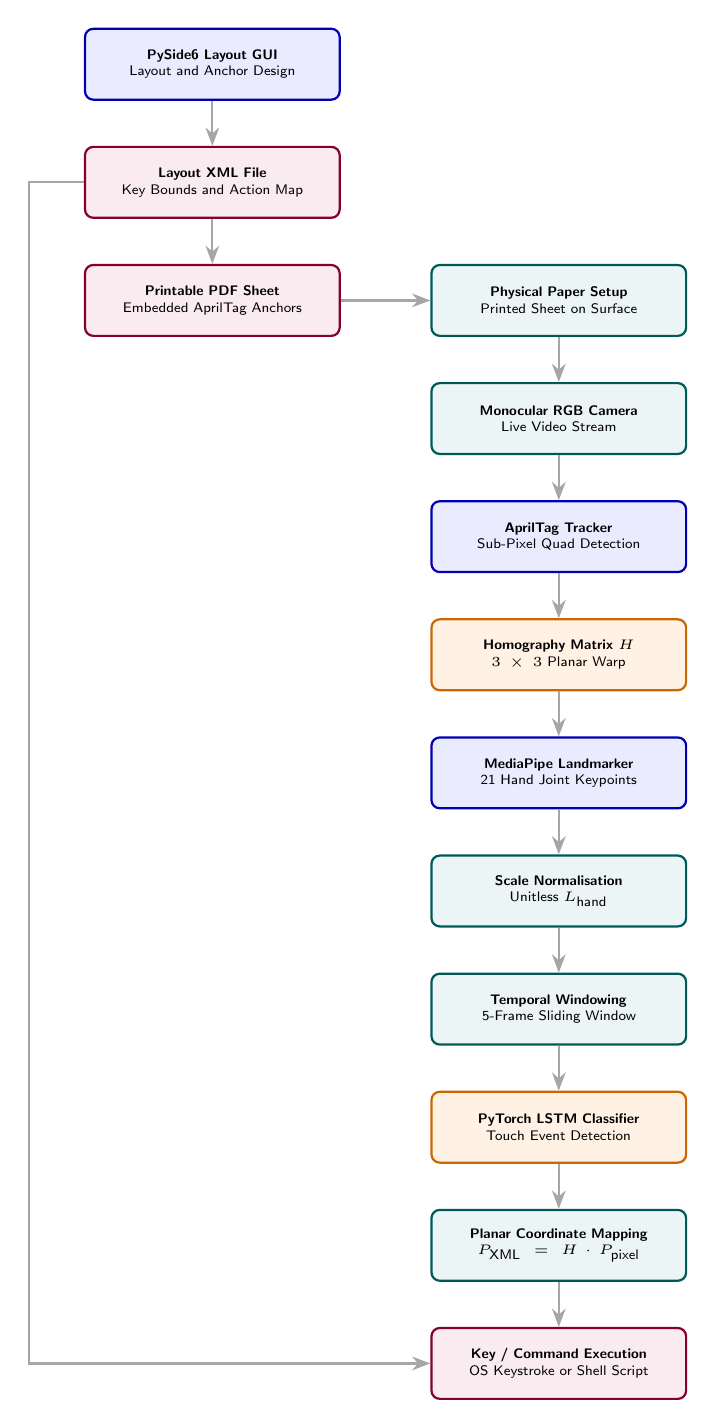
\begin{tikzpicture}[
    box/.style={draw=blue!70!black, rectangle, rounded corners=3pt,
                text width=3.0cm, minimum height=0.9cm, align=center,
                fill=blue!8!white, font=\sffamily\tiny, thick},
    process/.style={draw=teal!70!black, rectangle, rounded corners=3pt,
                text width=3.0cm, minimum height=0.9cm, align=center,
                fill=teal!8!white, font=\sffamily\tiny, thick},
    model/.style={draw=orange!80!black, rectangle, rounded corners=3pt,
                text width=3.0cm, minimum height=0.9cm, align=center,
                fill=orange!10!white, font=\sffamily\tiny, thick},
    artifact/.style={draw=purple!70!black, rectangle, rounded corners=3pt,
                text width=3.0cm, minimum height=0.9cm, align=center,
                fill=purple!8!white, font=\sffamily\tiny, thick},
    arrow/.style={-Stealth, thick, draw=gray!70}
]

%% ---- LEFT COLUMN: Offline Design Pipeline (x=0) ----
\node [box]      (designer)   at (0,  0)    {\textbf{PySide6 Layout GUI}\\Layout and Anchor Design};
\node [artifact] (xml)        at (0, -1.5)  {\textbf{Layout XML File}\\Key Bounds and Action Map};
\node [artifact] (pdf)        at (0, -3.0)  {\textbf{Printable PDF Sheet}\\Embedded AprilTag Anchors};

%% ---- RIGHT COLUMN: Online Runtime Pipeline (x=4.4) ----
\node [process]  (paper)      at (4.4, -3.0)  {\textbf{Physical Paper Setup}\\Printed Sheet on Surface};
\node [process]  (camera)     at (4.4, -4.5)  {\textbf{Monocular RGB Camera}\\Live Video Stream};
\node [box]      (apriltag)   at (4.4, -6.0)  {\textbf{AprilTag Tracker}\\Sub-Pixel Quad Detection};
\node [model]    (homography) at (4.4, -7.5)  {\textbf{Homography Matrix $H$}\\$3\times3$ Planar Warp};
\node [box]      (mediapipe)  at (4.4, -9.0)  {\textbf{MediaPipe Landmarker}\\21 Hand Joint Keypoints};
\node [process]  (norm)       at (4.4,-10.5)  {\textbf{Scale Normalisation}\\Unitless $L_{\text{hand}}$};
\node [process]  (window)     at (4.4,-12.0)  {\textbf{Temporal Windowing}\\5-Frame Sliding Window};
\node [model]    (lstm)       at (4.4,-13.5)  {\textbf{PyTorch LSTM Classifier}\\Touch Event Detection};
\node [process]  (mapping)    at (4.4,-15.0)  {\textbf{Planar Coordinate Mapping}\\$P_{\text{XML}}=H\cdot P_{\text{pixel}}$};
\node [artifact] (execution)  at (4.4,-16.5)  {\textbf{Key / Command Execution}\\OS Keystroke or Shell Script};

%% ---- LEFT COLUMN ARROWS ----
\draw [arrow] (designer) -- (xml);
\draw [arrow] (xml)      -- (pdf);

%% ---- BRIDGE: PDF to physical paper ----
\draw [arrow] (pdf.east) -- (paper.west);

%% ---- RIGHT COLUMN ARROWS ----
\draw [arrow] (paper)      -- (camera);
\draw [arrow] (camera)     -- (apriltag);
\draw [arrow] (apriltag)   -- (homography);
\draw [arrow] (homography) -- (mediapipe);
\draw [arrow] (mediapipe)  -- (norm);
\draw [arrow] (norm)       -- (window);
\draw [arrow] (window)     -- (lstm);
\draw [arrow] (lstm)       -- (mapping);
\draw [arrow] (mapping)    -- (execution);

%% ---- XML load feed ----
\draw [arrow] (xml.west) -- ++(-0.7,0) |- (execution.west);

\end{tikzpicture}%
}
\caption{Rich Picture of the Proposed Solution and Operational Pipeline Architecture.}
\label{fig:rich_picture_diagram}
\end{figure}

The pipeline executes through seven operational steps:
\begin{enumerate}
    \item \textbf{Layout Design and Export:} The user designs key boundaries and assigns commands using the PySide6 designer, exporting synchronized XML configuration and printable AprilTag PDF files.
    \item \textbf{Physical Setup:} The PDF layout is printed on standard paper, placed on a flat surface, and captured by an ordinary RGB webcam (see physical setup photographs and printable layout artifacts in Appendix~\ref{ch:appendix_physical_setup}).
    \item \textbf{AprilTag Tracking and Homography:} Corner fiducials are tracked to compute the $3 \times 3$ planar homography matrix $H$, mapping image pixels to layout coordinates \cite{Wang2016AprilTag2, Kallwies2020Determining}.
    \item \textbf{Hand Tracking and Normalization:} MediaPipe extracts 21 skeletal landmarks \cite{Zhang2020MediaPipe}, which are scale-normalized relative to unitless hand length ($L_{\text{hand}}$) without temporal smoothing.
    \item \textbf{Temporal Windowing:} Normalized coordinates and joint velocities are grouped into 5-frame sliding windows with 2-frame overlap at 12 FPS \cite{Simao2016Unsupervised}.
    \item \textbf{CPU-Based LSTM Touch Detection:} A compact PyTorch LSTM network evaluates each 5-frame sequence on the CPU, classifying touch probabilities across all five fingers independently \cite{Hochreiter1997LSTM, GilMartin2023Hand}.
    \item \textbf{Coordinate Mapping and Execution:} When touch contact is confirmed, fingertip pixel coordinates are transformed via $H$ into XML coordinates ($P_{\text{XML}} = H \cdot P_{\text{pixel}}$) to dispatch the corresponding key press or system command.
\end{enumerate}

\section{Resource Requirements}
\label{sec:resource_requirements}

\subsection{Hardware Requirements}
\label{subsec:hardware_req}
\begin{itemize}
    \item \textbf{Camera Sensor:} Standard USB webcam or integrated laptop camera supporting regular video resolutions. High-speed cameras or depth sensors are not required.
    \item \textbf{Host Computer:} Standard commodity PC or laptop with an x86\_64 or ARM processor (such as Intel Core i3/i5 or AMD Ryzen) and at least 4 GB of RAM.
    \item \textbf{Graphics Hardware:} Dedicated GPUs are not required; all runtime inference runs entirely on the host CPU.
    \item \textbf{Physical Media:} Standard desktop laser or inkjet printer using ordinary A4 or US Letter paper.
\end{itemize}

\subsection{Software Requirements}
\label{subsec:software_req}
\begin{itemize}
    \item \textbf{Operating System:} Linux (Ubuntu 22.04/24.04 LTS), macOS, or Windows 11.
    \item \textbf{Runtime Environment:} Python 3.10+ with the \texttt{uv} package manager.
    \item \textbf{GUI Framework:} PySide6 (Qt for Python) for the visual layout designer.
    \item \textbf{Computer Vision Libraries:} OpenCV and Pupil AprilTag for image processing and tag tracking.
    \item \textbf{Pose Estimation:} Google MediaPipe Hand Landmarker for skeletal joint extraction.
    \item \textbf{Deep Learning Framework:} PyTorch for LSTM sequence model training and CPU inference.
\end{itemize}

\section{Project Scope}
\label{sec:project_scope}
Table~\ref{tab:project_scope} defines the technical boundaries of the research.

\begin{table}[H]
\centering
\caption{System Project Scope Boundaries (In-Scope vs. Out-of-Scope)}
\label{tab:project_scope}
\small
\begin{tabularx}{\textwidth}{p{0.48\textwidth} p{0.48\textwidth}}
\toprule
\textbf{In-Scope System Elements} & \textbf{Out-of-Scope System Elements} \\
\midrule
Customizable paper-based virtual macro keyboard for application shortcuts, command execution, and macro tasks. & Direct replacement for general-purpose high-speed continuous prose typing keyboards. \\
\addlinespace
Single standard monocular RGB camera (USB or laptop webcam) operating at 12 FPS. & Depth cameras, Time-of-Flight sensors, infrared illuminators, or stereo camera rigs. \\
\addlinespace
Single active hand tracking with 21 landmarks, evaluating independent touch probabilities across all five fingers. & Bimanual (two-handed) typing, deferred to future work to avoid tag occlusion on compact A4 paper. \\
\addlinespace
Standard plain paper with four border AprilTag anchors printed via desktop printer (A4 or Letter). & Active capacitive overlays, conductive ink, wired panels, or electronic paper components. \\
\addlinespace
Real-time CPU inference on commodity processors without requiring dedicated GPUs. & High-end GPU workstations or cloud-based inference servers. \\
\addlinespace
PySide6 desktop application for designing custom layouts, exporting XML maps, and generating printable PDFs. & Mobile operating system apps (Android/iOS) or browser extensions. \\
\addlinespace
AprilTag fiducial tracking with $3 \times 3$ planar homography under perspective tilt. & Non-planar or curved 3D surfaces (such as cylinders or spheres). \\
\addlinespace
Unitless hand-length scale normalization ($L_{\text{hand}}$) with direct feature propagation for distance and scale invariance. & Biomechanical muscle force modeling or finger joint pressure estimation. \\
\addlinespace
Compact PyTorch LSTM sequence classifier using 5-frame sliding windows on CPU. & Large language model auto-correction or continuous text prediction engines. \\
\addlinespace
Real-time keystroke dispatch, shortcut hotkeys, shell scripts, and XML key boundary lookup. & Multi-user simultaneous input on a single paper sheet. \\
\bottomrule
\end{tabularx}
\end{table}

\subsection{In-Scope Technical Boundaries}
\label{subsec:in_scope_boundaries}
The system operates using a single standard monocular RGB webcam and plain printed paper without studio optics or depth sensors \cite{Posner2012Single, Sreenath2021Monocular}. Crucially, while prior monocular RGB keyboards were universally limited to single-finger interaction, this research presents the first monocular RGB virtual keyboard framework to achieve independent five-finger touch detection across all individual digits (Thumb, Index, Middle, Ring, Pinky) on a flat physical surface without requiring specialized 3D depth sensors or wearable markers. As an auxiliary macro controller rather than a general typing keyboard, discrete key taps eliminate the fatigue of continuous blind typing on flat surfaces.

Interaction is optimized for single-handed use, tracking 21 skeletal joints of one active hand while the user's other hand operates a mouse or primary keyboard. Single-handed tracking achieves 29.09 ms latency on commodity CPUs and avoids AprilTag occlusions on A4 paper. The PySide6 Layout Designer decouples geometry from actions, allowing one printed sheet to be bound to multiple action profiles (developer shortcuts, audio controls, shell scripts) without reprinting \cite{Doan2022Efficient, Lee2022Virtual}. AprilTag homography dynamically compensates for camera tilt up to $75^\circ$ and paper shifts \cite{Wang2016AprilTag2, Kalaitzakis2021Fiducial}. Landmarks are scale-normalized relative to hand length ($L_{\text{hand}}$) at 12 FPS and classified using the PyTorch LSTM model on CPU \cite{Zhang2020MediaPipe, GilMartin2023Hand}.

\subsection{Out-of-Scope Boundaries and Future Extensions}
\label{subsec:out_scope_boundaries}
To maintain low-cost deployment on commodity hardware, several elements remain outside scope. Direct replacement of mechanical keyboards for continuous prose typing is strictly out of scope, as blind continuous text entry requires mechanical switch travel that paper cannot deliver. Specialized hardware (ToF depth cameras, stereo rigs, infrared projectors, data gloves) is excluded \cite{Lee2019Virtual, Kudale2016RealTime}. Non-planar 3D surfaces are omitted, focusing strictly on flat desktop planes. Two-handed bimanual typing and multi-user input are deferred to future work to prevent AprilTag occlusion on standard A4 paper. Finally, physical touch force measurement and language model predictive auto-correction are reserved for future work.

\section{Chapter Summary}
\label{sec:chapter_summary}
This introductory chapter presented the research problem background, formal problem statement, primary research question and sub-questions, practical motivations, high-level operational pipeline, resource requirements, and project scope boundaries. By relying strictly on a single standard monocular RGB camera, plain printed paper with AprilTag anchors, and lightweight deep learning running on a commodity CPU, the framework addresses longstanding barriers in accessible human-computer interaction. The formal research objectives guiding the execution of this dissertation are detailed in Chapter~\ref{chap:objectives}.

\newpage
\chapter{Objectives}
\label{chap:objectives}

\section{General Objective}
\label{sec:general_objective}
The overarching objective of this research is to design, implement, and evaluate a customizable paper-based virtual macro keyboard system powered by a single standard monocular RGB camera and deep learning. Specifically engineered as an auxiliary macro controller for application shortcuts, command execution, and macro tasks rather than a replacement for general-purpose continuous typing keyboards, the system allows users to design custom macro layouts on normal paper and link different action combinations (such as application hotkeys, media controls, and system shell scripts) to the same physical printed sheet, executing entirely on standard commodity CPUs in real time without requiring dedicated GPUs, depth sensors, or specialized hardware accessories.

\section{Specific Objectives}
\label{sec:specific_objectives}
To accomplish the general research aim, the investigation is partitioned into the following specific research and engineering objectives:

\subsection{Objective 1: Theoretical Analysis and Baseline Requirements}
\label{subsec:obj1_theoretical}
To review and analyze existing visual input systems, fiducial marker tracking methods, planar homography algorithms, and hand pose estimation models. This establishes baseline technical requirements for monocular macro touch detection on flat printed paper without requiring specialized depth sensors, infrared illuminators, or rigid camera mounts.

\subsection{Objective 2: Hand Kinematic Representation and Scale Normalization}
\label{subsec:obj2_kinematics}
To investigate the spatial and temporal kinematic properties of human hand joints during macro touch contact, formulate a unitless hand-length scale normalization scheme ($L_{\text{hand}}$) invariant to camera distance and image resolution, and establish a standardized 12~FPS sliding temporal windowing pipeline (5 frames with 2-frame overlap) that preserves impact deceleration dynamics without introducing low-pass temporal filtering delays.

\subsection{Objective 3: Deep Learning Sequence Model Architecture Benchmark}
\label{subsec:obj3_deep_learning}
To benchmark, train, and optimize lightweight deep learning sequence architectures (comparing 1D CNN, Attention, ResNet, BiLSTM, and LSTM) for independent multi-finger macro touch contact classification, selecting an optimal neural network model that operates under 3~ms on a standard commodity CPU while achieving high touch detection precision and recall across all five digits.

\subsection{Objective 4: System Architecture Engineering and Two-Application Suite Design}
\label{subsec:obj4_suite_design}
To architect and implement an integrated two-application macro keyboard software suite:
\begin{enumerate}
    \item \textbf{Application 1 (Layout Designer Suite):} An interactive PySide6 graphical tool enabling users to define macro key boundaries, place border AprilTag fiducial anchors, and export synchronized layout XML definitions alongside printable vector PDF sheets.
    \item \textbf{Application 2 (Runtime Virtual Keyboard Engine):} An interactive action configuration GUI and real-time background vision engine that continuously tracks AprilTag fiducials to compute planar homography ($H$), extracts normalized skeletal landmarks via MediaPipe, classifies finger touch events using the PyTorch sequence model on CPU, and dispatches mapped application shortcuts, hotkeys, or system shell commands.
\end{enumerate}

\subsection{Objective 5: Empirical System Evaluation and Functional Benchmarking}
\label{subsec:obj5_evaluation}
To experimentally evaluate the complete virtual macro keyboard pipeline across touch detection classification accuracy (precision, recall, and F1-score), planar homography stability under perspective tilt and partial tag occlusion, end-to-end CPU execution latency on standard commodity hardware, and macro action dispatch verification across functional test cases FT-01 to FT-10.

\newpage
\chapter{Literature Review}
\label{ch:literature_review}

\section{Overview of the Chapter and Research Context}
\label{sec:lit_chapter_overview}
When I started doing research on input interfaces, I came to understand that most human-computer interactions still make use of key switches. The use of physical keyboards provides reliable tactile feedback for typing prose, but modern software and creative jobs need macro keypads and shortcut consoles \cite{ReviewVirtualKeyboard2020, Lee2022Virtual}. These include video editing consoles and developer launching pads. But commercially available hardware macro pads cost from \$100 to \$300, are not customizable in any way physically, and it is hard to maintain hygiene in them. This led researchers to look into the possibility of using virtual keyboards on flat surfaces by making use of computer vision \cite{Zhang2001Visual, Srivastava2012RealTime, Khare2019QWERTY, Maman2023TypeNet}. Although most early attempts have been made to create alternatives for continuous typing on paper, it was physically difficult to type on paper continuously without any tactile switch travel. For customizable macro controllers, paper works much better because users only glance at and tap individual shortcut buttons.

There were four huge challenges to getting a monocular paper virtual keyboard to work well:
\begin{itemize}
    \item \textbf{Surface Touch Detection Without Depth Sensors:} With standard 2D webcams it is impossible to measure depth in the Z-axis, making it difficult to differentiate between a real paper touch and a hovering finger \cite{Thomas2013Camera, Posner2012Single, Lee2019Virtual, Toshpulatov2024RealTime}.
    \item \textbf{Hand Scale and Perspective Variations:} Hand landmark coordinates vary according to different hand sizes and distances from the lens \cite{Zhang2020MediaPipe, Doan2022Efficient}. Normalizing coordinates is needed without adding lag from heavy smoothing filters \cite{Kumar2026Hybrid}.
    \item \textbf{Planar Orientation and Camera Tilt:} The perspective effect on the desk surface that comes from tilting the camera means we need to compute a planar homography matrix ($H \in \mathbb{R}^{3 \times 3}$) so as to keep key bounds aligned continuously \cite{Wang2016AprilTag2, Kallwies2020Determining, Pirchheim2011Homography}.
    \item \textbf{Decoupled Layout Design and Action Multiplexing:} Older systems hardcoded QWERTY layouts rather than allowing users to pair various software action profiles with one printed sheet \cite{ReviewVirtualKeyboard2020}.
\end{itemize}

In order to lay a sound foundation, this chapter analyzes the current literature across four main categories. Firstly, I define the literature framework and searching methodology. Secondly, I discuss the evolution of input devices and the biomechanical aspects of finger strikes. Thirdly, I conduct a comparative analysis of existing virtual keyboards from eight different sensing mechanisms and analyze their drawbacks. Lastly, I examine the mathematical and algorithmic aspects of MediaPipe hand tracking, scale normalization, AprilTag homography, and PyTorch LSTM touch detection, leading to the research gaps that motivate this thesis.

\section{Conceptual Map of the Literature}
\label{sec:lit_conceptual_map}
In Figure~\ref{fig:lit_conceptual_map_diagram}, I plotted the literature against four primary pillars: HCI input approaches, sensing types, technical algorithms, and synthesis of research gaps.

\begin{figure}[htbp]
\centering
\resizebox{\textwidth}{!}{%
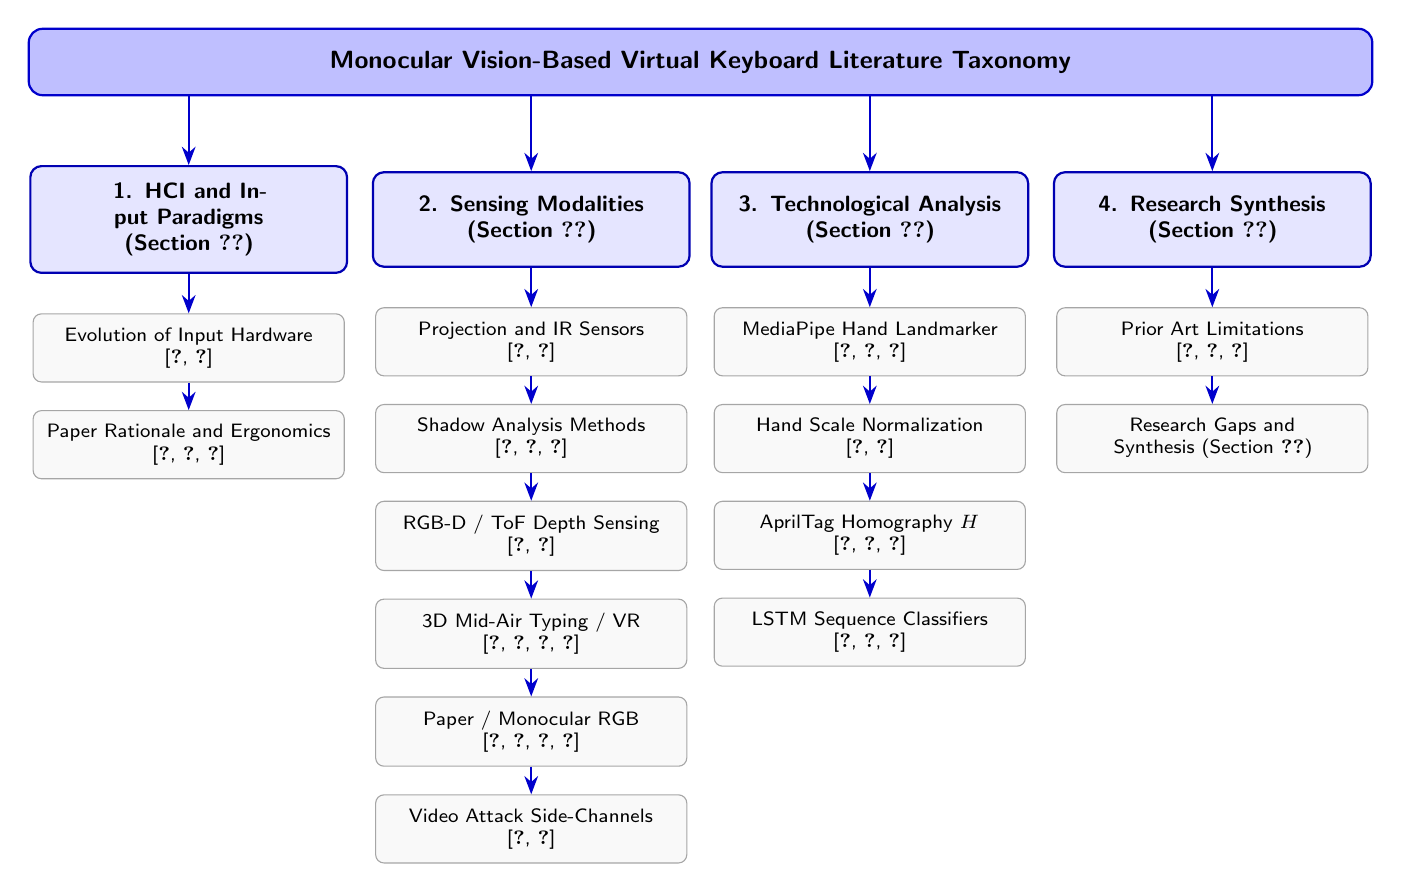
\begin{tikzpicture}[
    header/.style = {rectangle, draw=blue!80!black, fill=blue!25!white, thick, rounded corners=5pt, align=center, font=\sffamily\bfseries\small, inner sep=8pt, text width=16.5cm},
    box/.style = {rectangle, draw=blue!70!black, fill=blue!10!white, thick, rounded corners=4pt, align=center, font=\sffamily\bfseries\footnotesize, inner sep=6pt, text width=3.6cm, minimum height=1.2cm},
    subbox/.style = {rectangle, draw=gray!70, fill=gray!5!white, rounded corners=3pt, align=center, font=\sffamily\scriptsize, inner sep=5pt, text width=3.6cm},
    arrow/.style = {draw=blue!80!black, ->, >=Stealth, thick}
]

% Root Node
\node (root) [header, at={(0, 0)}] {\textbf{Monocular Vision-Based Virtual Keyboard Literature Taxonomy}};

% Level 1 Nodes
\node (l1_domain) [box, at={(-6.5, -2.0)}] {1. HCI and Input Paradigms\\(Section~\ref{sec:lit_domain_overview})};
\node (l1_systems) [box, at={(-2.15, -2.0)}] {2. Sensing Modalities\\(Section~\ref{sec:lit_existing_systems})};
\node (l1_tech) [box, at={(2.15, -2.0)}] {3. Technological Analysis\\(Section~\ref{sec:lit_technological_analysis})};
\node (l1_reflect) [box, at={(6.5, -2.0)}] {4. Research Synthesis\\(Section~\ref{sec:lit_reflection})};

% Connections to Level 1
\draw [arrow] (root.south -| l1_domain.north) -- (l1_domain.north);
\draw [arrow] (root.south -| l1_systems.north) -- (l1_systems.north);
\draw [arrow] (root.south -| l1_tech.north) -- (l1_tech.north);
\draw [arrow] (root.south -| l1_reflect.north) -- (l1_reflect.north);

% Column 1: Domain Overview
\node (l2_history) [subbox, below=0.5cm of l1_domain] {Evolution of Input Hardware\\\cite{ReviewVirtualKeyboard2020, Lee2022Virtual}};
\node (l2_drivers) [subbox, below=0.35cm of l2_history] {Paper Rationale and Ergonomics\\\cite{Zhang2001Visual, Srivastava2012RealTime, Khare2019QWERTY}};

% Column 2: Existing Systems
\node (l2_proj) [subbox, below=0.5cm of l1_systems] {Projection and IR Sensors\\\cite{Cheng2015Fingertip, Kudale2016RealTime}};
\node (l2_shadow) [subbox, below=0.35cm of l2_proj] {Shadow Analysis Methods\\\cite{Thomas2013Camera, Posner2012Single, Yue2014Blind}};
\node (l2_depth) [subbox, below=0.35cm of l2_shadow] {RGB-D / ToF Depth Sensing\\\cite{Lee2019Virtual, Toshpulatov2024RealTime}};
\node (l2_air) [subbox, below=0.35cm of l2_depth] {3D Mid-Air Typing / VR\\\cite{Boletsis2019TextInput, Enkhbat2020HandKey, Lee2022Virtual, Yoo2026WordLevel}};
\node (l2_paper) [subbox, below=0.35cm of l2_air] {Paper / Monocular RGB\\\cite{Zhang2001Visual, Srivastava2012RealTime, Khare2019QWERTY, Maman2023TypeNet}};
\node (l2_attack) [subbox, below=0.35cm of l2_paper] {Video Attack Side-Channels\\\cite{Yue2014Blind, Yang2022Towards}};

% Column 3: Technological Analysis
\node (l2_pose) [subbox, below=0.5cm of l1_tech] {MediaPipe Hand Landmarker\\\cite{Zhang2020MediaPipe, GilMartin2023Hand, Andriyanov2025Improving}};
\node (l2_scale) [subbox, below=0.35cm of l2_pose] {Hand Scale Normalization\\\cite{Doan2022Efficient, Kumar2026Hybrid}};
\node (l2_fiducial) [subbox, below=0.35cm of l2_scale] {AprilTag Homography $H$\\\cite{Wang2016AprilTag2, Kallwies2020Determining, Pirchheim2011Homography}};
\node (l2_deep) [subbox, below=0.35cm of l2_fiducial] {LSTM Sequence Classifiers\\\cite{Hochreiter1997LSTM, Nunez2018Convolutional, Gammulle2021TMMF}};

% Column 4: Research Synthesis
\node (l2_gap) [subbox, below=0.5cm of l1_reflect] {Prior Art Limitations\\\cite{Thomas2013Camera, Lee2019Virtual, Maman2023TypeNet}};
\node (l2_solution) [subbox, below=0.35cm of l2_gap] {Research Gaps and\\Synthesis (Section~\ref{sec:lit_reflection})};

% Vertical Column Connections
\draw [arrow] (l1_domain) -- (l2_history);
\draw [arrow] (l2_history) -- (l2_drivers);

\draw [arrow] (l1_systems) -- (l2_proj);
\draw [arrow] (l2_proj) -- (l2_shadow);
\draw [arrow] (l2_shadow) -- (l2_depth);
\draw [arrow] (l2_depth) -- (l2_air);
\draw [arrow] (l2_air) -- (l2_paper);
\draw [arrow] (l2_paper) -- (l2_attack);

\draw [arrow] (l1_tech) -- (l2_pose);
\draw [arrow] (l2_pose) -- (l2_scale);
\draw [arrow] (l2_scale) -- (l2_fiducial);
\draw [arrow] (l2_fiducial) -- (l2_deep);

\draw [arrow] (l1_reflect) -- (l2_gap);
\draw [arrow] (l2_gap) -- (l2_solution);

\end{tikzpicture}%
}
\caption{Conceptual taxonomy and structural organization of the literature review.}
\label{fig:lit_conceptual_map_diagram}
\end{figure}

The review is structured across four main themes:
\begin{itemize}
    \item \textbf{HCI and Input Paradigms (Section~\ref{sec:lit_domain_overview}):} Evolution of input hardware, biomechanics of finger-surface impact, and user performance metrics.
    \item \textbf{Sensing Modalities (Section~\ref{sec:lit_existing_systems}):} Critical evaluation of eight sensing technologies, synthesized in Table~\ref{tab:lit_comparative_matrix}.
    \item \textbf{Technological Analysis (Section~\ref{sec:lit_technological_analysis}):} Mathematical formulation and algorithmic analysis of hand tracking, scale normalization, fiducial homography, and deep learning touch detection.
    \item \textbf{Research Synthesis (Section~\ref{sec:lit_reflection}):} Identification of the six fundamental literature gaps and the formal research problem statement.
\end{itemize}

\subsection{Literature Search Strategy and PRISMA 2020 Systematic Protocol}
\label{subsec:lit_search_strategy}
For the systematic review process, I applied the PRISMA 2020 protocol through IEEE Xplore, ACM Digital Library, Scopus, Elsevier ScienceDirect, and Google Scholar to find peer-reviewed studies from 2000 to 2025 \cite{ReviewVirtualKeyboard2020}:
\begin{enumerate}
    \item \textbf{Search Syntax:} I searched with queries containing: \texttt{("virtual keyboard" OR "paper keyboard") AND ("monocular RGB" OR "MediaPipe") AND ("touch detection" OR "homography")}.
    \item \textbf{Inclusion Criteria:} I added peer-reviewed papers that showed functioning virtual keyboards, planar contact algorithms, fiducial tracking with tilt, or real-time hand joint estimation.
    \item \textbf{Exclusion Criteria:} I removed papers that required wearable sensor gloves, intrusive markers, multi-camera motion capture rigs, or were only conceptual white papers without implementation.
    \item \textbf{Synthesis Approach:} The shortlisted papers were then compared on the basis of sensing approaches, multi-finger support, compute latency, and environmental robustness to identify the problem areas this project addresses.
\end{enumerate}

\section{Domain Overview}
\label{sec:lit_domain_overview}

\subsection{Evolution of Text Entry and Spatial HCI Hardware}
\label{subsec:lit_history_evolution}
Considering the evolution of text input, early mechanical keyboards used physical switches that provided key travel with strong tactile feedback \cite{ReviewVirtualKeyboard2020}. Next came membrane keyboards, where production became cheaper, and capacitive touchscreens that offered soft visual key layouts without physical tactile edges \cite{ReviewVirtualKeyboard2020}. Optical laser keyboards projected the outline of keys using infrared light \cite{Cheng2015Fingertip, Kudale2016RealTime}; however, these could not work reliably in bright environments as ambient light would wash out the pattern. Nowadays, entering complex command sequences can be done by dedicated macro pads (such as the Stream Deck), which enable users to trigger multi-key shortcuts with one keypress. However, such devices are expensive (usually priced from \$100 up to \$300) while being non-modifiable physically. Monocular computer vision allows us to track 21 hand joints using only a standard webcam \cite{Zhang2020MediaPipe, GilMartin2023Hand}, which means we can use a printed piece of paper as an inexpensive, customizable macro pad without active electronics.

\subsection{Kinematic Typing Dynamics and Biomechanical Surface Impact}
\label{subsec:lit_typing_biomechanics}
Without a depth sensor, I needed to understand the physical characteristics of a finger as it makes contact with a flat desk in order to identify touch events \cite{Simao2016Unsupervised, MacRitchie2015Integrating, Pilkov2024Markerless}. A physical keystroke consists of four kinematic phases:
\begin{enumerate}
    \item \textbf{Approaching Phase ($t_1$ to $t_2$):} The finger moves downward at increasing vertical speed towards the target button ($V_y$).
    \item \textbf{Impact Phase ($t_2$ to $t_3$):} When encountering the rigid paper surface, downward velocity is zeroed in 20 to 40~ms ($V_y \to 0$), producing a steep deceleration spike ($A_y = \frac{dV_y}{dt} \ll 0$).
    \item \textbf{Resting Phase ($t_3$ to $t_4$):} The finger pauses briefly on the paper while the touch event registers.
    \item \textbf{Recoil Phase ($t_4$ to $t_5$):} The finger rebounds upward away from the desk surface ($V_y > 0$).
\end{enumerate}
The rigid desk acts as a hard physical boundary, providing immediate deceleration of motion. Conversely, fingers tend to overshoot in mid-air typing systems, as there is no stopping surface \cite{Boletsis2019TextInput, Maman2023TypeNet}.

\subsection{Ergonomics and Human Input Performance Metrics}
\label{subsec:lit_fitts_law}
Input performance by humans has a direct correlation with physical feedback and movement dynamics:
\begin{itemize}
    \item \textbf{Tactile Key Travel versus Discrete Visual Targeting:} With a mechanical keyboard, a depth of keystroke between $2\text{ to }4\text{ mm}$ allows fast blind touch-typing without needing to see the keys. On flat paper, typing continuous prose creates strain on fingers since there is no mechanical key travel \cite{ReviewVirtualKeyboard2020}. For macro keypads, people do not type continuous prose; rather, they look for a particular button and press it once. The presence of custom button sizes on paper layouts directly improves ergonomics.
    \item \textbf{Discrete Macro Action Rate versus Continuous Typing Speed:} Traditional typing tests measure input speed in Words Per Minute based on continuous character sequences. In contrast, for macro keypads, touch accuracy and reduced latency are the critical performance metrics rather than continuous typing speed.
    \item \textbf{Keystrokes Per Character (KSPC):} Efficiency is measured by Keystrokes Per Character. Physical keyboards generally register about 1.05 KSPC, while contactless mid-air keyboards have more than 1.30 KSPC owing to accidental touches \cite{Boletsis2019TextInput}.
    \item \textbf{Fitts' Law:} Fitts' Law models how long it takes to reach a target button of width $W$ at distance $D$ through the Index of Difficulty ($ID$) in bits:
    \begin{equation}
    MT = a + b \log_2 \left( 1 + \frac{D}{W} \right) = a + b \cdot ID
    \label{eq:fitts_law}
    \end{equation}
    The customizable paper macro keyboard enables one to customize the button width $W$ in the software designer, directly reducing the Index of Difficulty for rapid shortcut selection.
\end{itemize}

\subsection{Multi-Finger Tendon Coupling}
\label{subsec:lit_biomechanical_coupling}
Anatomical tendon coupling in the human hand is another biological factor \cite{Simao2016Unsupervised, Pilkov2024Markerless}. Shared muscle pathways are found in the flexor and extensor tendons of the middle, ring, and pinky fingers. For example, when someone presses down with one finger, the fingers next to it involuntarily twitch downward. These minor twitches are confused for intentional key presses by basic single-finger tracking algorithms \cite{Thomas2013Camera, Srivastava2012RealTime}. Deep sequence models address this by tracking combinations of movement from all 21 hand joints over time to differentiate intentional taps from passive tendon twitches.

\section{Existing Systems and Sensing Modalities}
\label{sec:lit_existing_systems}
Reviewing previous systems of virtual keyboards, one may note that eight different sensing modalities have been explored.

\subsection{Projection-Based and Infrared Sensor Systems}
\label{subsec:lit_proj_systems}
Projection keyboards use a red laser grid placed on the table surface and sense finger presence as an invisible infrared beam is broken \cite{Cheng2015Fingertip, Kudale2016RealTime}. Kudale and Wanjale \cite{Kudale2016RealTime} implemented an infrared camera tracking reflective markers using four-point homography. However, the ambient light of the room destroys the pattern through wash-out and makes changing the key arrangement impossible.

\subsection{Shadow-Based Monocular RGB Keyboards}
\label{subsec:lit_shadow_systems}
Monocular RGB shadow sensors calculate the distance between the fingertip and its cast shadow, which reaches zero upon physical contact \cite{Thomas2013Camera, Posner2012Single, Yue2014Blind}. Posner et al. \cite{Posner2012Single} applied adaptive shadow thresholding for paper contact detection. However, shadow analysis fails under diffuse lighting, multiple light sources, or dark desk surfaces \cite{Yue2014Blind}. Crucially, shadow methods completely fail when several fingers move simultaneously because their shadows overlap and merge.

\subsection{Hardware-Assisted Depth Sensors (RGB-D and ToF)}
\label{subsec:lit_depth_systems}
Depth sensors like Microsoft Kinect, Intel RealSense, and Time-of-Flight cameras create metric 3D point clouds \cite{Lee2019Virtual, Toshpulatov2024RealTime}. Lee and Kwon \cite{Lee2019Virtual} calibrated a flat surface to detect touches when fingertip point clouds crossed a distance threshold. Toshpulatov et al. \cite{Toshpulatov2024RealTime} combined 3D depth information and optical flow to filter out hovering artifacts. However, depth cameras are costly, power-hungry, prone to noise close to flat surfaces, and require dedicated GPUs to process in real-time.

\subsection{3D Mid-Air Typing and AR/VR Virtual Keyboards}
\label{subsec:lit_air_systems}
Spatial computing headsets have spurred interest in mid-air keyboards \cite{Boletsis2019TextInput, Enkhbat2020HandKey, Lee2022Virtual, Yoo2026WordLevel}. Enkhbat et al. \cite{Enkhbat2020HandKey} introduced HandKey, detecting typing within 3D bounding cubes. Lee et al. \cite{Lee2022Virtual} tracked two-handed mid-air typing for head-mounted displays. However, mid-air typing lacks a physical desk surface where fingers stop; therefore, users experience high levels of arm fatigue and overshoot target keys \cite{Boletsis2019TextInput, Maman2023TypeNet}.

\subsection{Paper-Anchored Monocular RGB Keyboards}
\label{subsec:lit_paper_systems}
Monocular paper keyboards employ standard webcams to interact virtually with printed paper sheets \cite{Zhang2001Visual, Srivastava2012RealTime, Khare2019QWERTY, Maman2023TypeNet}. Zhang et al. \cite{Zhang2001Visual} tracked page corners to compute planar homography. Vertical velocity thresholds of pixels were employed by Srivastava and Tripathi \cite{Srivastava2012RealTime}, while a printed QWERTY sheet was tracked by Khare \cite{Khare2019QWERTY} employing skin-color segmentation. TypeNet \cite{Maman2023TypeNet} enabled typing on uncalibrated surfaces with deep keypoint tracking. However, all prior monocular paper keyboards were limited in that they detected the movement of only one finger at a time.

\subsection{Specialized and Assistive Modalities}
\label{subsec:lit_specialized_assistive}
Additional forms of sensing involve VLC photodiodes \cite{Webber2021Finger}, fingernail color-based blood volume imaging \cite{Sun2009Estimation}, optical motion capture \cite{MacRitchie2015Integrating, Pilkov2024Markerless}, and gaze tracking \cite{Chen2024Gaze}. Gaze tracking assists people with motor disabilities, although the Midas Touch effect causes unintended key clicks while stopping to read \cite{Chen2024Gaze}.

\subsection{Fiducial Tracking in Planar Robotics}
\label{subsec:lit_robotics_systems}
With regard to tracking technology, planar robotics research proves that square fiducial markers like AprilTag and ArUco offer sub-pixel tracking accuracy even when the camera is tilted severely \cite{Ivacko2024Edge, Herdiansyah2024Implementation, Schenck2024Utilizing, GarridoJurado2026ArUco}. Ivacko et al. \cite{Ivacko2024Edge} utilized ArUco markers for mapping robot coordinate frames, while Garrido-Jurado et al. \cite{GarridoJurado2026ArUco} realized high frame rate contour scanning.

\subsection{Comparative Literature Analysis Matrix}
\label{subsec:lit_comparative_matrix}
Some examples of previous work in terms of sensing modality, hardware requirements, tracking techniques, scale normalization, temporal filtering, touch classification, and layout flexibility are presented in Table~\ref{tab:lit_comparative_matrix}. Importantly, across all monocular RGB-based approaches operating on physical surfaces, none support multi-finger interaction; multi-finger input was previously available only in expensive depth camera setups or virtual reality environments.

\begin{table}[htbp]
\centering
\caption{Comparative analysis of existing virtual keyboard frameworks and sensing methodologies.}
\label{tab:lit_comparative_matrix}
\resizebox{\textwidth}{!}{%
\begin{tabular}{l l l l l l l l l}
\toprule
\textbf{Study and Year} & \textbf{Sensing Modality} & \textbf{Hardware Req.} & \textbf{Surface Tracking} & \textbf{Scale Normalization} & \textbf{Temporal Filter} & \textbf{Touch Classifier} & \textbf{Latency / FPS} & \textbf{Layout Customization} \\
\midrule
Zhang et al. (2001) \cite{Zhang2001Visual} & Monocular RGB & Standard Webcam & Quad Paper Bounds & None (Pixel Coords) & Moving Avg. & Spatial Proximity & High ($\sim 15$ FPS) & Rigid Paper Quad \\
Sun et al. (2009) \cite{Sun2009Estimation} & Monocular RGB & High-Res Camera & None (Fixed Finger) & None & None & LDA Nail Coloration & Offline ($< 5$ FPS) & None \\
Pirchheim and Reitmayr (2011) \cite{Pirchheim2011Homography} & Monocular RGB & Mobile Camera & Keyframe Homography & Feature Scale & Particle Filter & Spatial Tracking & Real-Time ($30$ FPS) & None (SLAM Map) \\
Srivastava and Tripathi (2012) \cite{Srivastava2012RealTime} & Monocular RGB & Standard Webcam & Manual Quad Contour & None (Raw Pixels) & Static Smoothing & Speed Deceleration & Real-Time ($25$ FPS) & Manual Paper Drawing \\
Posner et al. (2012) \cite{Posner2012Single} & Monocular RGB & Standard Webcam & Fixed Desk Layout & None & Dynamic Threshold & Fingertip-Shadow Dist. & Real-Time ($30$ FPS) & Fixed Paper Template \\
Thomas (2013) \cite{Thomas2013Camera} & Monocular RGB & Standard Webcam & Fixed Area & None & None & Shadow Gradient Vector & Real-Time ($30$ FPS) & Fixed Layout \\
Yue et al. (2014) \cite{Yue2014Blind} & Monocular RGB & Smartphone RGB & Screen Border H & None & Optical Flow & Shadow + k-Means & Offline Analysis & Fixed Smartphone Screen \\
Cheng et al. (2015) \cite{Cheng2015Fingertip} & Proj. + Camera & Projector + Camera & Photometric Calib. & None & Background Sub. & 3D Shadow Distance & Real-Time ($20$ FPS) & Fixed Projected GUI \\
MacRitchie and McPherson (2015) \cite{MacRitchie2015Integrating} & Optical MoCap & MoCap + Touch & Surface Calibration & 3D Skeleton mm & Moving Average & Velocity Inversion & Real-Time ($100$ FPS) & Fixed Piano Keys \\
Kudale and Wanjale (2016) \cite{Kudale2016RealTime} & IR Webcam & IR Filtered Camera & 4-Point Homography & None & Thresholding & IR Pen Tap Contact & Real-Time ($30$ FPS) & Projected Display \\
Simao et al. (2017) \cite{Simao2016Unsupervised} & Motion Capture & Leap Motion Sensor & None & Bone Lengths & Sliding Window & Velocity Inversion & Real-Time ($60$ FPS) & None \\
Ji et al. (2018) \cite{Ji2018Local} & Monocular RGB & Standard Webcam & Skin Color Mask & None & Moving Avg. & k-Means Clustering & Real-Time ($25$ FPS) & Dynamic Key Clusters \\
Nunez et al. (2018) \cite{Nunez2018Convolutional} & 3D Skeleton & Depth Sensor & None & Normalized Skeleton & Sequence Window & CNN + LSTM Network & Real-Time ($30$ FPS) & None \\
Lai and Yanushkevich (2018) \cite{Lai2018CNN} & Multimodal RGB-D & Depth Sensor & None & Skeleton Joint Map & Temporal Buffer & CNN + RNN Fusion & Real-Time ($30$ FPS) & Gesture Set \\
Khare (2019) \cite{Khare2019QWERTY} & Monocular RGB & Standard Webcam & Static Bounds & None & Color Threshold & Pause Over Bounds & Real-Time ($20$ FPS) & Fixed QWERTY Paper \\
Lee and Kwon (2019) \cite{Lee2019Virtual} & RGB-D Depth & ToF Depth Camera & Depth Plane Calib. & 3D Metric mm & Weight Filtering & Z-Depth Threshold & Real-Time ($30$ FPS) & Fixed Virtual Touch \\
Boletsis and Kongsvik (2019) \cite{Boletsis2019TextInput} & VR Controller & VR Headset & Virtual 3D Grid & VR World Scale & None & Striking Velocity & Real-Time ($90$ FPS) & Fixed VR Layout \\
Enkhbat et al. (2020) \cite{Enkhbat2020HandKey} & Monocular RGB & Standard Webcam & Air Typing Zone & Hand Size Scaling & None & CNN Spatial Classifier & Real-Time ($30$ FPS) & Fixed Air QWERTY \\
Cui et al. (2020) \cite{Cui2020Deep} & Vision Review & Various Sensors & Various & Various & Various & Deep Learning Survey & N/A & N/A \\
Zhang et al. (2020) \cite{Zhang2020MediaPipe} & Monocular RGB & Commodity Camera & Palm Detector & Normalized 21 Keypoints & Single-frame Regress & Skeletal Keypoint Reg. & High Speed ($> 60$ FPS) & General Hand Tracking \\
Ikram and Liu (2020) \cite{Ikram2020Skeleton} & 3D Skeleton & Leap Motion Sensor & None & Hand Scale & Sliding Window & 1D CNN + LSTM & Real-Time ($50$ FPS) & Mid-air Gestures \\
Wang et al. (2020) \cite{Wang2020Relative} & Monocular RGB & Stereo Pair & Superpixel Homography & Superpixel Scale & Bundle Adjust & Multi-Model RANSAC & Real-Time ($25$ FPS) & Planar Maps \\
Li et al. (2021) \cite{Li2021CNN} & Monocular RGB & Embedded Camera & Grid Mask & None & CNN Feature Map & Lightweight CNN & Edge Real-Time ($30$ FPS) & Fixed Key Grid \\
Webber et al. (2021) \cite{Webber2021Finger} & Visible Light & VLC Photodiodes & Optical Intensity Mask & None & Intensity Features & SVM / Random Forest & Real-Time ($30$ FPS) & Light Grid Keys \\
Gammulle et al. (2021) \cite{Gammulle2021TMMF} & Multimodal RGB & Single Camera & None & Sequence Normalization & Multi-Modal Fusion & Single-Stage TMMF Net & Real-Time ($30$ FPS) & Continuous Gestures \\
Zhang et al. (2022) \cite{Zhang2022DynaKey} & Head-Mounted RGB & Smart Glasses & Gyro + Homography & None & Motion Compensation & Downward Trajectory & Real-Time ($30$ FPS) & Drawn Keyboard Bounds \\
Lee et al. (2022) \cite{Lee2022Virtual} & RGB-D / HMD & AR/VR Headset & HMD Frame & 3D Joint Scaling & Temporal Buffer & 7-Class Deep Network & Real-Time ($60$ FPS) & Ambidextrous Layouts \\
Doan (2022) \cite{Doan2022Efficient} & Monocular RGB & Commodity RGB & None & Scale Normalized & Coordinate Smooth & Multi-layer LSTM & Real-Time ($30$ FPS) & Body Activity \\
Yang et al. (2022) \cite{Yang2022Towards} & Smartphone RGB & Commodity Phone & Uncalibrated Video & Self-Supervised Scale & Motion Trajectory & Deep Inference Model & Offline Analysis & Uncalibrated Keyboards \\
Maman and Bermano (2023) \cite{Maman2023TypeNet} & Monocular RGB & Front Camera & Uncalibrated Plane & Hand Skeleton Scale & Self-Refinement & Deep Net + LM Decoding & Real-Time ($30$ FPS) & Fixed QWERTY Flat \\
Gil-Martin et al. (2023) \cite{GilMartin2023Hand} & Monocular RGB & Commodity Camera & None & MediaPipe Scale & Sequence Buffer & Deep Recurrent Net & Real-Time ($60$ FPS) & General Gestures \\
Sanchez-Brizuela et al. (2023) \cite{SanchezBrizuela2023Lightweight} & Monocular RGB & Commodity Camera & None & Landmark Distance & Morphological Mask & Landmark Rule Classifier & Ultra High ($90$ FPS) & Skin Segmentation \\
Ivacko et al. (2024) \cite{Ivacko2024Edge} & Monocular RGB & Wrist Camera & ArUco Calibration & Metric Scaling & Low-Pass Alpha & Rule-Based Kinematics & Edge Real-Time ($30$ FPS) & Robot Control Pad \\
Herdiansyah et al. (2024) \cite{Herdiansyah2024Implementation} & Monocular RGB & Single RGB Camera & ArUco PnP & Metric Tag Size & Zhang Calibration & Geometric Pose Engine & Real-Time ($30$ FPS) & Navigation Targets \\
Pilkov (2024) \cite{Pilkov2024Markerless} & Multi-Camera RGB & 3 RGB Cameras & None & 3D Skeleton mm & Temporal Alignment & Deep Keypoint Trajectory & Real-Time ($30$ FPS) & Piano Keyboard \\
Toshpulatov et al. (2024) \cite{Toshpulatov2024RealTime} & Multimodal RGB-D & Depth + RGB & Surface Calib. & 3D Spatial mm & Fusion Filter & Temporal Depth-Motion Net & Real-Time ($30$ FPS) & VR/AR GUI Objects \\
Chen (2024) \cite{Chen2024Gaze} & Monocular RGB & Commodity Webcam & Screen Grid & Pupil Vector Scale & Dwell Time Filter & Eye-Gaze Deep Model & Real-Time ($30$ FPS) & Gaze Keypad \\
Schenck et al. (2024) \cite{Schenck2024Utilizing} & Monocular RGB & Single RGB Camera & ArUco Inpainting & Metric Scale & Inpainting Mask & Deep Keypoint Detector & Real-Time ($30$ FPS) & Robotic Links \\
Andriyanov et al. (2025) \cite{Andriyanov2025Improving} & Monocular RGB & Commodity RGB & Bounding Box & Normalized Bounds & Temporal Window & MediaPipe + YOLO-Pose & Real-Time ($45$ FPS) & Gesture Set \\
Yoo and Lee (2026) \cite{Yoo2026WordLevel} & Monocular RGB & Single RGB Camera & None & Trajectory Scaling & Displacement Accum. & Word Motion Network & Real-Time ($30$ FPS) & Contactless QWERTY \\
Kumar (2026) \cite{Kumar2026Hybrid} & Monocular RGB & Commodity Camera & Canvas Plane & Landmark Ratio & Adaptive Low-Pass & Motion Threshold & Real-Time ($60$ FPS) & Air Canvas Drawing \\
Garrido-Jurado et al. (2026) \cite{GarridoJurado2026ArUco} & Monocular RGB & Commodity Camera & ArUco Nano Tags & Metric Tag Scale & Sub-pixel Sampling & Visited-Aware Contours & Edge High ($> 100$ FPS) & Robotics Targets \\
\bottomrule
\end{tabular}%
}
\end{table}

\section{Technological Analysis}
\label{sec:lit_technological_analysis}
This section analyzes the four foundational technical modules: skeletal hand tracking, scale normalization, planar homography, and deep learning touch classification.

\subsection{Hand Pose Estimation and Skeletal Joint Tracking}
\label{subsec:lit_hand_pose}
Markerless hand tracking is a must for natural interactions without sensors on the hand \cite{Cui2020Deep, Zhang2020MediaPipe}. Initially, color thresholding was attempted in HSV space \cite{Ji2018Local, Khare2019QWERTY}, but this failed as light conditions changed or due to differences in skin tones. Google MediaPipe Hands \cite{Zhang2020MediaPipe} resolves this problem with the help of a two-stage deep learning process optimized to work well on regular CPUs:
\begin{enumerate}
    \item \textbf{Single-Shot Palm Detector:} A one-shot palm detector finds a bounding box for the palm region across the entire image using focal loss $\mathcal{L}_{\text{focal}} = -\alpha_t (1 - p_t)^\gamma \log(p_t)$. By focusing on the rigid palm region rather than articulating finger movement, tracking loss is minimized.
    \item \textbf{Hand Landmark Model:} The cropped palm region feeds into a hand landmark model that predicts 3D coordinates $(x_i, y_i, z_i)$ for 21 skeletal joints (Figure~\ref{fig:mediapipe_hand_topology}).
\end{enumerate}

\begin{figure}[htbp]
\centering
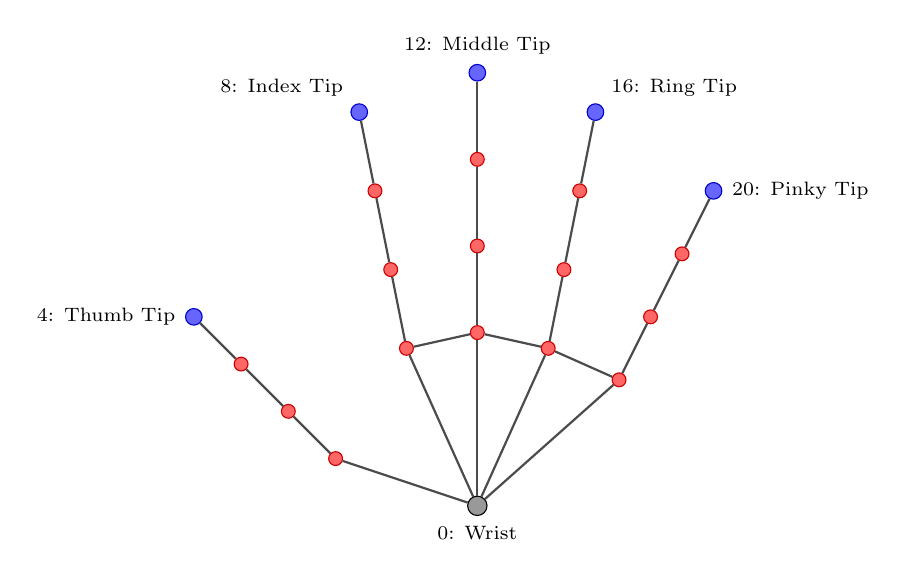
\begin{tikzpicture}[
    joint/.style = {circle, draw=red!80!black, fill=red!60!white, inner sep=0pt, minimum size=5pt},
    tip/.style = {circle, draw=blue!80!black, fill=blue!60!white, inner sep=0pt, minimum size=6pt},
    wrist/.style = {circle, draw=black, fill=gray!80, inner sep=0pt, minimum size=7pt},
    bone/.style = {draw=black!70, thick}
]

% Wrist
\node (J0) [wrist, label=below:{\scriptsize 0: Wrist}] at (0, 0) {};

% Thumb
\node (J1) [joint] at (-1.8, 0.6) {};
\node (J2) [joint] at (-2.4, 1.2) {};
\node (J3) [joint] at (-3.0, 1.8) {};
\node (J4) [tip, label=left:{\scriptsize 4: Thumb Tip}] at (-3.6, 2.4) {};

% Index Finger
\node (J5) [joint] at (-0.9, 2.0) {};
\node (J6) [joint] at (-1.1, 3.0) {};
\node (J7) [joint] at (-1.3, 4.0) {};
\node (J8) [tip, label=above left:{\scriptsize 8: Index Tip}] at (-1.5, 5.0) {};

% Middle Finger
\node (J9) [joint] at (0.0, 2.2) {};
\node (J10) [joint] at (0.0, 3.3) {};
\node (J11) [joint] at (0.0, 4.4) {};
\node (J12) [tip, label=above:{\scriptsize 12: Middle Tip}] at (0.0, 5.5) {};

% Ring Finger
\node (J13) [joint] at (0.9, 2.0) {};
\node (J14) [joint] at (1.1, 3.0) {};
\node (J15) [joint] at (1.3, 4.0) {};
\node (J16) [tip, label=above right:{\scriptsize 16: Ring Tip}] at (1.5, 5.0) {};

% Pinky Finger
\node (J17) [joint] at (1.8, 1.6) {};
\node (J18) [joint] at (2.2, 2.4) {};
\node (J19) [joint] at (2.6, 3.2) {};
\node (J20) [tip, label=right:{\scriptsize 20: Pinky Tip}] at (3.0, 4.0) {};

% Bones Connections
\draw [bone] (J0) -- (J1) -- (J2) -- (J3) -- (J4);
\draw [bone] (J0) -- (J5) -- (J6) -- (J7) -- (J8);
\draw [bone] (J0) -- (J9) -- (J10) -- (J11) -- (J12);
\draw [bone] (J0) -- (J13) -- (J14) -- (J15) -- (J16);
\draw [bone] (J0) -- (J17) -- (J18) -- (J19) -- (J20);
\draw [bone] (J5) -- (J9) -- (J13) -- (J17);

\end{tikzpicture}
\caption{MediaPipe 21 hand landmark anatomical topology.}
\label{fig:mediapipe_hand_topology}
\end{figure}

MediaPipe provides five fingertip coordinates (Landmarks 4, 8, 12, 16, 20) and knuckle base joints (MCP, PIP, DIP) with execution speeds greater than 60~FPS on standard CPUs \cite{GilMartin2023Hand, SanchezBrizuela2023Lightweight}.

\subsection{Kinematic Scale Normalization and Raw Feature Propagation}
\label{subsec:lit_scale_norm}
Landmark pixel positions vary with the distance between the user's hand and the webcam, along with the actual size of the hand \cite{Doan2022Efficient, Kumar2026Hybrid}. With respect to the standard pinhole camera model of projection:
\begin{equation}
x_{\text{pixel}} = f \frac{X}{Z}, \quad y_{\text{pixel}} = f \frac{Y}{Z}
\label{eq:pinhole_projection}
\end{equation}

Scaling camera distance by factor $k$ ($Z' = k Z$) implies inverse scaling of pixel positions:
\begin{equation}
x'_{\text{pixel}} = \frac{x_{\text{pixel}}}{k}, \quad y'_{\text{pixel}} = \frac{y_{\text{pixel}}}{k}, \quad L'_{\text{hand}} = \frac{L_{\text{hand}}}{k}
\label{eq:pixel_scaling}
\end{equation}
where $L_{\text{hand}}$ is the reference hand length defined as the Euclidean distance between the wrist $\mathbf{P}_0 = (x_0, y_0)$ and the middle MCP knuckle $\mathbf{P}_9 = (x_9, y_9)$:
\begin{equation}
L_{\text{hand}} = \sqrt{(x_9 - x_0)^2 + (y_9 - y_0)^2}
\label{eq:hand_length_scale_def}
\end{equation}

Scaling landmark displacements with respect to the wrist reference $\mathbf{P}_0$ by hand length $L_{\text{hand}}$ eliminates the influence of scale variations:
\begin{equation}
\mathbf{P}_i^{\text{norm}\prime} = \frac{\mathbf{P}_i' - \mathbf{P}_0'}{L'_{\text{hand}}} = \frac{\frac{\mathbf{P}_i - \mathbf{P}_0}{k}}{\frac{L_{\text{hand}}}{k}} = \frac{\mathbf{P}_i - \mathbf{P}_0}{L_{\text{hand}}} = \mathbf{P}_i^{\text{norm}}
\label{eq:scale_invariance_proof}
\end{equation}

First-order numerical velocities are calculated between consecutive frames:
\begin{equation}
\mathbf{V}_i(t) = \frac{\mathbf{P}_i^{\text{norm}}(t) - \mathbf{P}_i^{\text{norm}}(t - \Delta t)}{\Delta t}
\label{eq:joint_velocity_def}
\end{equation}

While mid-air gesture recognition employs filtering techniques to remove jittering \cite{Kumar2026Hybrid}, this cannot be applied to touch detection as smoothing filters destroy the 40~ms deceleration spike ($A_y \ll 0$) upon surface contact and introduce 30 to 90~ms of added latency.

\subsection{Planar Homography and Fiducial Tracking}
\label{subsec:lit_homography}
In order to map camera pixel coordinates into the coordinate system of the printed paper, distortion needs to be removed using a $3 \times 3$ planar homography matrix $H$ \cite{LonguetHiggins1985Machine, Pirchheim2011Homography, Wang2020Relative}:
\begin{equation}
\begin{bmatrix}
x_{\text{XML}} w \\
y_{\text{XML}} w \\
w
\end{bmatrix}
=
H \mathbf{P}_{\text{pixel}}
=
\begin{bmatrix}
h_{11} & h_{12} & h_{13} \\
h_{21} & h_{22} & h_{23} \\
h_{31} & h_{32} & h_{33}
\end{bmatrix}
\begin{bmatrix}
x_{\text{pixel}} \\
y_{\text{pixel}} \\
1
\end{bmatrix}
\label{eq:homography_equation_def}
\end{equation}

The projective scaling factor $w$ allows obtaining Cartesian coordinates on paper:
\begin{equation}
x_{\text{XML}} = \frac{h_{11} x_{\text{pixel}} + h_{12} y_{\text{pixel}} + h_{13}}{h_{31} x_{\text{pixel}} + h_{32} y_{\text{pixel}} + h_{33}}, \quad
y_{\text{XML}} = \frac{h_{21} x_{\text{pixel}} + h_{22} y_{\text{pixel}} + h_{23}}{h_{31} x_{\text{pixel}} + h_{32} y_{\text{pixel}} + h_{33}}
\label{eq:homography_cartesian_def}
\end{equation}

A minimum of four corner correspondences between detected fiducial markers and the printed sheet forms an overdetermined linear system $\mathbf{A}_{8 \times 9} \mathbf{h} = \mathbf{0}$, resolved through Singular Value Decomposition (SVD) \cite{Wang2016AprilTag2, Kallwies2020Determining}.

In experimental results provided by Kalaitzakis et al. \cite{Kalaitzakis2021Fiducial}, AprilTag provides a smaller error of corner localization ($0.017\text{ pixels}$) compared to ArUco and ARTag, even at a camera tilt of $75^\circ$, running in under $1.0\text{ ms}$ on standard commodity CPUs without GPU hardware.

\subsection{Deep Sequential Touch Detection Models}
\label{subsec:lit_deep_touch}
A simple velocity threshold approach ($V_y > \theta$) cannot reliably detect touch due to hand hovering and tendon coupling between fingers \cite{Simao2016Unsupervised, Toshpulatov2024RealTime}. Long Short-Term Memory (LSTM) recurrent neural networks \cite{Hochreiter1997LSTM} retain internal memory over time, thus providing the perfect fit for classifying kinetic impact:
\begin{align}
\mathbf{f}_t &= \sigma(\mathbf{W}_f [\mathbf{h}_{t-1}, \mathbf{x}_t] + \mathbf{b}_f) \label{eq:lstm_forget_def} \\
\mathbf{i}_t &= \sigma(\mathbf{W}_i [\mathbf{h}_{t-1}, \mathbf{x}_t] + \mathbf{b}_i) \label{eq:lstm_input_def} \\
\tilde{\mathbf{C}_t} &= \tanh(\mathbf{W}_c [\mathbf{h}_{t-1}, \mathbf{x}_t] + \mathbf{b}_c) \label{eq:lstm_candidate_def} \\
\mathbf{C}_t &= \mathbf{f}_t \odot \mathbf{C}_{t-1} + \mathbf{i}_t \odot \tilde{\mathbf{C}_t} \label{eq:lstm_cell_def} \\
\mathbf{o}_t &= \sigma(\mathbf{W}_o [\mathbf{h}_{t-1}, \mathbf{x}_t] + \mathbf{b}_o) \label{eq:lstm_output_def} \\
\mathbf{h}_t &= \mathbf{o}_t \odot \tanh(\mathbf{C}_t) \label{eq:lstm_hidden_def}
\end{align}

Recurrent models for sequence learning consider joint movements in sliding temporal windows, examining multi-frame sequences rather than a single static image \cite{Nunez2018Convolutional, Ikram2020Skeleton, Doan2022Efficient}. This separates downward descent, physical surface contact, and finger rebound cleanly.

\subsection{System Architecture Sensing Trade-Offs}
\label{subsec:lit_sensing_tradeoffs}
Table~\ref{tab:lit_sensing_tradeoffs} compares the architectural trade-offs across common optical and physical sensing modalities evaluated in virtual input literature.

\begin{table}[htbp]
\centering
\caption{System architecture design trade-offs across sensing modalities.}
\label{tab:lit_sensing_tradeoffs}
\resizebox{\textwidth}{!}{%
\begin{tabular}{l l l l l}
\toprule
\textbf{Architectural Dimension} & \textbf{Monocular RGB + Planar Fiducials} & \textbf{RGB-D / ToF Depth Sensing} & \textbf{Laser Projection + IR} & \textbf{3D Mid-Air Typing (VR)} \\
\midrule
\textbf{Hardware Sensor Cost} & Low (Commodity Webcam) & High (\$150 to \$400 Depth Camera) & Medium (\$80 to \$150 Projector) & High (\$400 to \$3500 Headset) \\
\textbf{Ambient Light Sensitivity} & Moderate (Robust to indoor lux) & High (Sunlight IR interference) & Extreme (Sunlight washes pattern) & Low (Built-in HMD sensors) \\
\textbf{Surface Alignment} & Dynamic (AprilTag Homography) & Fixed Depth Plane Calibration & Fixed Desktop Projection & None (Mid-air tracking) \\
\textbf{Tactile Feedback} & Passive Surface Tactile Stop & Passive Surface Tactile Stop & Passive Surface Tactile Stop & Complete Absence (Fatigue) \\
\textbf{Layout Customization} & High (Printable XML Layouts) & Moderate (Fixed Spatial GUI) & Low (Hardcoded Laser Pattern) & High (Software VR Grids) \\
\textbf{Edge Compute Latency} & Low ($> 60$ FPS on CPU) & Medium (Point Cloud Compute) & Low (Hardware IR Processing) & High (Heavy HMD Pipeline) \\
\bottomrule
\end{tabular}%
}
\end{table}

As illustrated in the comparison, monocular RGB sensing with planar fiducials strikes a strong balance between low hardware unit cost, passive desk tactile contact without requiring specialized active sensors, and customizable planar layout tracking relative to active depth sensors or projection hardware.

\section{Reflection and Synthesis of Research Gaps}
\label{sec:lit_reflection}

\subsection{Synthesis of Prior Literature Limitations}
\label{subsec:lit_synthesis_limitations}
However, there are some common problems that can be seen from the discussed systems. Firstly, for monocular systems in physical desktops, previous systems could only track one finger per time, maybe an index fingertip \cite{Zhang2001Visual, Srivastava2012RealTime, Posner2012Single, Thomas2013Camera, Ji2018Local, Khare2019QWERTY}. In the event where users move multiple fingers simultaneously, shadow detection will not work because of the overlapping shadows \cite{Posner2012Single, Yue2014Blind}, and 2D pixel detection will not be able to distinguish the depth of each finger that is coming down.

In order to cope with the lack of depth information, previous 2D systems had to impose pauses of $500\text{ to }1000\text{ ms}$ on each keystroke (dwell time) \cite{Khare2019QWERTY, Chen2024Gaze}, thus making typing very slow and disrupting natural interaction flow. Also, deep neural networks require fast GPUs to run and do not work well on commodity CPUs, achieving fewer than 15~FPS \cite{Enkhbat2020HandKey, Ji2018Local}.

A further concern is the lighting-sensitive nature of the problem. Simple room lights, hand shadows, and variations in skin complexions break down the segmentation and skin color detection process \cite{Thomas2013Camera, Yue2014Blind}. In order to overcome this challenge, several researchers resorted to using expensive three-dimensional sensors, infrared projectors, or even wearable devices like gloves with sensors \cite{Lee2019Virtual, Kudale2016RealTime, Toshpulatov2024RealTime, Pilkov2024Markerless}, yet this approach defeats the purpose of using an inexpensive vision system. Finally, virtually all vision keyboards from earlier work use fixed QWERTY keyboards \cite{Maman2023TypeNet, Enkhbat2020HandKey}. They lack custom-printed keyboards with fiducials, nor do they offer mapping of multiple software profiles to one piece of paper.

\subsection{Formal Research Gap Justification}
\label{subsec:lit_gap_justification}
These drawbacks bring into focus the primary problem that the current work aims at solving; it is the construction of an adaptive paper-based macro keyboard by means of solely a regular monocular RGB camera and a commodity CPU. The key requirements include the detection of multi-touch hits without any additional dwell times, utilization of AprilTag planar homography ($H$) for tracking the paper's position, and providing users with options for defining different software actions on a single printed layout.

This can be done by integrating the techniques of layout design using visualization, planar homography, unit-independent scaling ($L_{\text{hand}}$), direct feature passing, and a light-weighted PyTorch LSTM sequence model, as described in the subsequent chapters.

\section{Summary of the Literature and Research Foundations}
\label{sec:lit_chapter_summary}
This chapter provided an overview of the prior body of knowledge in the areas of virtual input devices, hand pose tracking, planar fiducials, and deep learning touch detection. Past studies on input devices technologies, typing effects on biomechanics, and ergonomics measurement were reviewed. Comparative analysis was conducted by comparing eight sensing approaches using a comparative matrix, whereas the MediaPipe algorithm, scale normalization, AprilTag homography, and PyTorch LSTM sequence classification algorithms were discussed. Finally, the six research questions answered in this thesis were summarized. These principles serve as direct inputs for the methodology and architecture presented in Chapter~\ref{ch:methodology}.

\newpage
\chapter{Methodology}
\label{ch:methodology}

\section{Chapter Overview}
\label{sec:meth_chapter_overview}
Crafting a paper-based virtual macro keyboard, for use with shortcuts and run commands using just a regular webcam and deep learning you need proper principled approach in terms of engineering methodology. This system is built to be an auxiliary macro keypad for application shortcuts, command execution, and custom tool palettes, unlike traditional physical keyboards intended for general continuous prose typing. The printed sheet has no physical or electronic switches; rather, discrete user touch interactions are detected in real time via computer vision, perspective homography, scale-normalized hand tracking, and neural network sequence classification running on commodity consumer computer processors (no GPU required).

This chapter outlines the research methods, system design and engineering pipelines. The outline of the research framework as an overview is described in Section~\ref{sec:meth_framework}, which is an application of Saunders' Research Onion being applied along with Design Science Research Methodology (DSRM). The generic architecture of the two-application system is described in Section~\ref{sec:meth_architecture} and Application~1 (Layout Designer Suite), which generates the key geometry and fiducial anchors, is introduced in Section~\ref{sec:meth_layout_designer}. In Section~\ref{sec:meth_data_pipeline}, we describe the video collection, sub-sampling (12~FPS), MediaPipe landmark tracking, unitless scale normalization and sliding temporal windowing. The sequence classification formulations and the PyTorch LSTM architecture are covered in Section~\ref{sec:meth_dl_models}. Application~2 (Runtime Engine), planar homography, coordinate lookup and action multiplexing are then defined in Section~\ref{sec:meth_runtime_engine}, while the chapter is rounded up in Section~\ref{sec:meth_summary}.

\section{Research Framework and Scientific Methodology}
\label{sec:meth_framework}

\subsection{Research Paradigm and Deductive Reasoning}
\label{subsec:meth_paradigm}
The present research focuses on Empirical Positivism and Pragmatism along with a Deductive Logical Reasoning Approach. In the domain of computer vision and Human-Computer Interaction, this includes finger kinematics, homography matrices, and deceleration effects. Positivism permits measuring and quantifying these physical events (precision, recall, F1-scores, Root Mean Square reprojection error in millimeters, and latency time in milliseconds) through reproducible laboratory measurements. The approach takes a pragmatic stance, achieving real-time interaction on commodity CPUs without requiring expensive GPUs or specialized depth cameras. Deductive reasoning maps formal mathematical theorems to software implementations:
\begin{enumerate}
    \item \textbf{Planar Homography Theory:} Four points on the paper plane are enough to compute a unique $3 \times 3$ matrix $H$, which is the homography matrix accounting for camera tilt angles and displacement of the paper across the desk \cite{Pirchheim2011Homography}.
    \item \textbf{Perspective Scale Invariance:} Normalizing landmark coordinates with respect to anatomical hand length ($L_{\text{hand}}$) makes classification invariant to distance and camera resolution.
    \item \textbf{Kinematic Impact Deceleration:} Physical surface contact causes an abrupt transition in velocity from downward motion to zero ($V_y \to 0$). Without specialized depth sensors, touch events can be detected through velocity classification across temporal intervals.
\end{enumerate}

\subsection{Methodological Grounding via Saunders' Research Onion}
\label{subsec:meth_saunders_onion}
The methodology is based on the six layers of Saunders' Research Onion \cite{ReviewVirtualKeyboard2020}, organizing and structuring the research procedure from philosophy through data analysis:
\begin{itemize}
    \item \textbf{Layer 1 (Research Philosophy):} Positivism and Pragmatism, evaluating objective empirical metrics such as latency, F1-scores, and accuracy on commodity hardware.
    \item \textbf{Layer 2 (Research Approach):} Deductive logic, deriving mathematical equations of planar perspective transformation and temporal deceleration validated with empirical data.
    \item \textbf{Layer 3 (Research Strategy):} A hybrid of Design Science Research Methodology (DSRM) and experimental laboratory benchmarking of modular software artifacts.
    \item \textbf{Layer 4 (Methodological Choice):} Quantitative empirical research assessing classification accuracy, throughput, and execution latency.
    \item \textbf{Layer 5 (Time Horizon):} Cross-sectional study design examining the system under specific camera tilt angles, lighting conditions, and video resolutions.
    \item \textbf{Layer 6 (Techniques and Procedures):} 12~FPS video capture, 21-landmark tracking, unitless scale normalization ($L_{\text{hand}}$), 5-frame temporal windowing, PyTorch LSTM training, and planar homography ($H$).
\end{itemize}

\subsection{Design Science Research Methodology (DSRM)}
\label{subsec:meth_dsrm}
The software engineering and development process adheres to the six stages of Design Science Research Methodology (DSRM) \cite{ReviewVirtualKeyboard2020}, as shown in Figure~\ref{fig:dsrm_process_flow}.

\begin{figure}[htbp]
\centering
\resizebox{0.92\textwidth}{!}{%
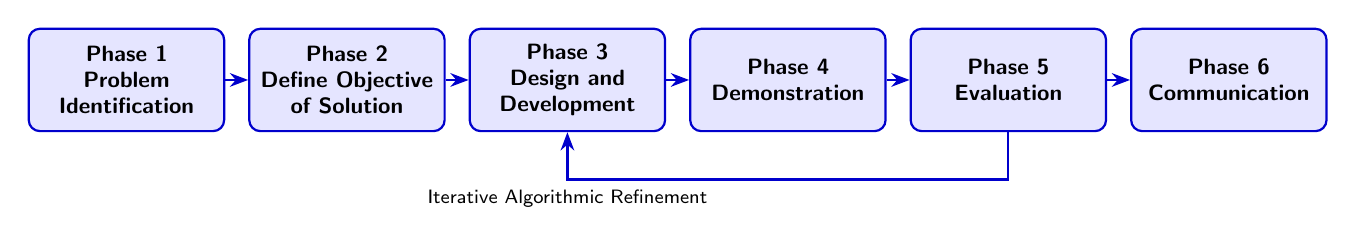
\begin{tikzpicture}[
    phase/.style = {rectangle, draw=blue!80!black, fill=blue!10!white, thick, rounded corners=4pt, align=center, font=\sffamily\bfseries\footnotesize, text width=2.2cm, minimum height=1.3cm, inner sep=4pt},
    arrow/.style = {draw=blue!80!black, ->, >=Stealth, thick}
]
\node (p1) [phase] at (0,0) {Phase 1\\Problem\\Identification};
\node (p2) [phase] at (2.8,0) {Phase 2\\Define Objective\\of Solution};
\node (p3) [phase] at (5.6,0) {Phase 3\\Design and\\Development};
\node (p4) [phase] at (8.4,0) {Phase 4\\Demonstration};
\node (p5) [phase] at (11.2,0) {Phase 5\\Evaluation};
\node (p6) [phase] at (14.0,0) {Phase 6\\Communication};

\draw [arrow] (p1) -- (p2);
\draw [arrow] (p2) -- (p3);
\draw [arrow] (p3) -- (p4);
\draw [arrow] (p4) -- (p5);
\draw [arrow] (p5) -- (p6);
\draw [arrow] (p5.south) -- ++(0,-0.6) -| node[below,midway,font=\sffamily\scriptsize]{Iterative Algorithmic Refinement} (p3.south);
\end{tikzpicture}%
}
\caption{Design Science Research Methodology (DSRM) execution framework.}
\label{fig:dsrm_process_flow}
\end{figure}

The steps of DSRM were performed in the following way:
\begin{itemize}
    \item \textbf{Phase 1: Problem Identification:} Identified virtual keyboard limitations: depth sensor hardware costs, shadow detection failures, rigid mounts, and single-finger limits.
    \item \textbf{Phase 2: Objectives Formulation:} Defined quantitative targets: CPU latency $< 83.33\text{ ms}$ at 12~FPS, multi-finger touch F1-score $> 0.94$, and macro action profile multiplexing.
    \item \textbf{Phase 3: Design and Development:} Constructed the two-application suite: Application~1 (Layout Designer) and Application~2 (Runtime Engine), which integrates MediaPipe, scale normalization, AprilTag homography, and PyTorch LSTM inference.
    \item \textbf{Phase 4: Demonstration:} Deployed the system on flat desks using plain printed paper and an ordinary USB webcam.
    \item \textbf{Phase 5: Evaluation:} Profiled CPU latency, throughput, and macro dispatch across functional test cases FT-01 through FT-10 for a total of 22 sequence models.
    \item \textbf{Phase 6: Communication:} Documented system architecture, empirical findings, and design insights in this dissertation.
\end{itemize}

\subsection{Partitioned Development and Experimental Strategy}
\label{subsec:meth_partitions}
Engineering of this project was carried out through five technical experimental partitions:
\begin{enumerate}
    \item \textbf{Partition 1 (Design Layout and Homography Simulation):} An early prototype was built (\texttt{designer\_app.py}) to assess the effectiveness of homography matrix mapping in \texttt{designer/analyzer/} prior to developing the modular layout designer in \texttt{virtualKeyboardSetup/designer/}.
    \item \textbf{Partition 2 (Dataset Preparation and Pipeline Engineering):} Scripts were written in \texttt{dataPipeline/src/} for data preprocessing to resample video at 12~FPS, extract 21 hand joints, perform unitless scale normalization ($L_{\text{hand}}$), calculate joint velocities, and construct 5-frame temporal sliding windows.
    \item \textbf{Partition 3 (Benchmarking Deep Learning Models):} Benchmarked 22 pure 2D deep learning models across 5 model families using \texttt{modelBenchmark/benchmark\_engine.py}, selecting \texttt{best\_finger\_touch\_lstm.pth}.
    \item \textbf{Partition 4 (Real-Time Responsiveness Testing):} Evaluated multi-threaded latency and trigger stability scripts on commodity CPU in \texttt{virtualKeyboardSetup/detector/}.
    \item \textbf{Partition 5 (AprilTag Fiducial Tracking):} Implemented corner detection and planar homography tracking in \texttt{aprilTag/} to maintain coordinate tracking up to $75^\circ$ perspective tilt.
\end{enumerate}

\section{System Architecture and Software Design}
\label{sec:meth_architecture}
The virtual keyboard achieves modularity by decoupling layout design from runtime execution. Figure~\ref{fig:system_architecture_framework} shows the system architecture connecting the workflows of both applications.

\begin{figure}[htbp]
\centering
\resizebox{0.92\textwidth}{!}{%
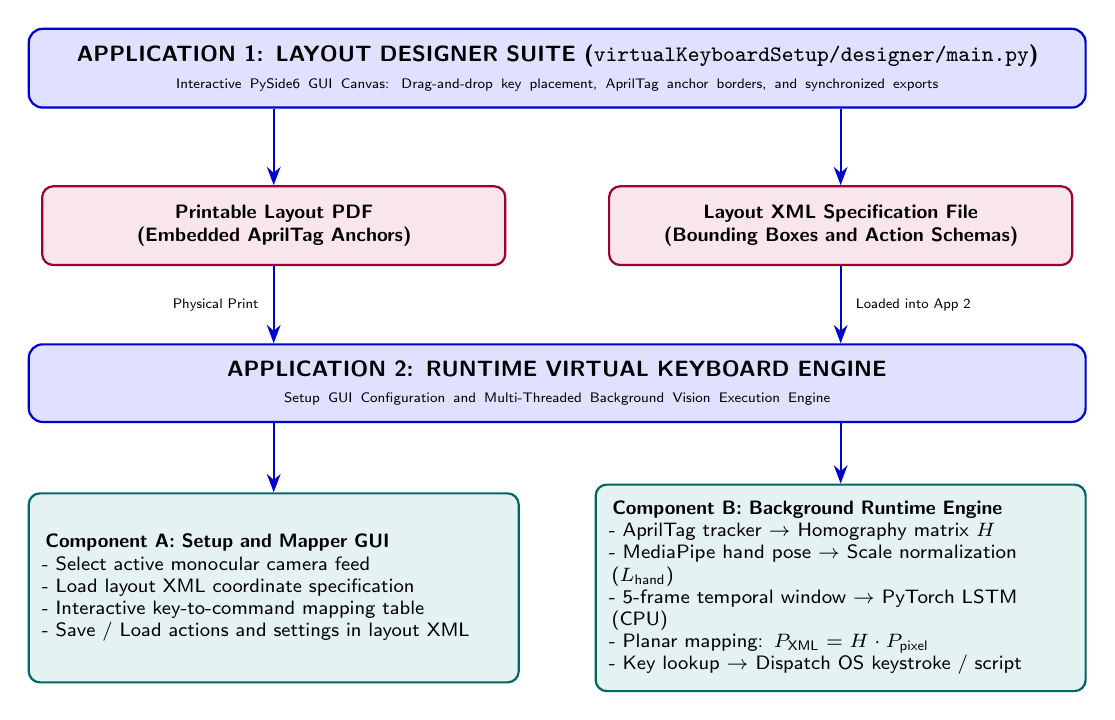
\begin{tikzpicture}[
    node distance = 1.2cm and 1.5cm,
    appbox/.style = {rectangle, draw=blue!80!black, fill=blue!12!white, thick, rounded corners=5pt, align=center, font=\sffamily\bfseries\footnotesize, text width=13.0cm, inner sep=6pt},
    artbox/.style = {rectangle, draw=purple!80!black, fill=purple!10!white, thick, rounded corners=4pt, align=center, font=\sffamily\bfseries\scriptsize, text width=5.6cm, minimum height=1.0cm, inner sep=4pt},
    compbox/.style = {rectangle, draw=teal!80!black, fill=teal!10!white, thick, rounded corners=4pt, align=left, font=\sffamily\scriptsize, text width=5.8cm, minimum height=2.4cm, inner sep=6pt},
    arrow/.style = {draw=blue!80!black, ->, >=Stealth, thick}
]

\node (app1) [appbox] at (0, 0) {
\textbf{APPLICATION 1: LAYOUT DESIGNER SUITE (\texttt{virtualKeyboardSetup/designer/main.py})}\\
{\normalfont\sffamily\tiny Interactive PySide6 GUI Canvas: Drag-and-drop key placement, AprilTag anchor borders, and synchronized exports}
};

\node (pdf_art) [artbox] at (-3.6, -2.0) {Printable Layout PDF\\(Embedded AprilTag Anchors)};
\node (xml_art) [artbox] at (3.6, -2.0) {Layout XML Specification File\\(Bounding Boxes and Action Schemas)};

\node (app2) [appbox] at (0, -4.0) {
\textbf{APPLICATION 2: RUNTIME VIRTUAL KEYBOARD ENGINE}\\
{\normalfont\sffamily\tiny Setup GUI Configuration and Multi-Threaded Background Vision Execution Engine}
};

\node (comp_a) [compbox] at (-3.6, -6.6) {
\textbf{Component A: Setup and Mapper GUI}\\
- Select active monocular camera feed\\
- Load layout XML coordinate specification\\
- Interactive key-to-command mapping table\\
- Save / Load actions and settings in layout XML
};

\node (comp_b) [compbox] at (3.6, -6.6) {
\textbf{Component B: Background Runtime Engine}\\
- AprilTag tracker $\to$ Homography matrix $H$\\
- MediaPipe hand pose $\to$ Scale normalization ($L_{\text{hand}}$)\\
- 5-frame temporal window $\to$ PyTorch LSTM (CPU)\\
- Planar mapping: $P_{\text{XML}} = H \cdot P_{\text{pixel}}$\\
- Key lookup $\to$ Dispatch OS keystroke / script
};

\draw [arrow] (app1.south -| pdf_art.north) -- (pdf_art.north);
\draw [arrow] (app1.south -| xml_art.north) -- (xml_art.north);
\draw [arrow] (pdf_art.south) -- node[left, font=\sffamily\tiny, align=right]{Physical Print\ } (app2.north -| pdf_art.south);
\draw [arrow] (xml_art.south) -- node[right, font=\sffamily\tiny, align=left]{\ Loaded into App 2} (app2.north -| xml_art.south);
\draw [arrow] (app2.south -| comp_a.north) -- (comp_a.north);
\draw [arrow] (app2.south -| comp_b.north) -- (comp_b.north);

\end{tikzpicture}%
}
\caption{System architecture framework connecting Application 1 and Application 2 workflows.}
\label{fig:system_architecture_framework}
\end{figure}

Software engineering design patterns ensure modularity, stability, and responsiveness on standard commodity computers:
\begin{enumerate}
    \item \textbf{Model-View-Controller (MVC):} In Application~1, this separates the interactive drawing canvas (View) from key coordinate data structures (Model) and mouse editing events (Controller).
    \item \textbf{Producer-Consumer Multi-Threading:} In Application~2, a dedicated camera background thread (\texttt{camera\_thread.py}) captures webcam video frames and places them into a frame queue, while the vision engine (\texttt{model\_manager.py}) processes frames asynchronously to prevent dropped frames and UI freezes.
    \item \textbf{Strategy Pattern for Action Dispatching:} Key press triggers are encapsulated as interchangeable action classes, enabling seamless switching between virtual OS keystroke simulations and system shell scripts.
    \item \textbf{Singleton Model Registry:} The trained PyTorch touch detection model (\texttt{best\_finger\_touch\_lstm.pth}) is loaded into CPU memory once at startup, eliminating reinitialization delays during typing.
\end{enumerate}

\section{Application 1: Layout Designer Suite}
\label{sec:meth_layout_designer}
Application~1 (\texttt{virtualKeyboardSetup/designer/main.py}) is an interactive graphical PySide6 application built for custom macro keyboard layout design. For regular desktop printers, standard A4 paper ($210 \times 297\text{ mm}$) is used by default, while custom formats like A3 and US Letter are also supported. The system was realized through exploratory prototypes early on (\texttt{designer/designer\_app.py}), followed by the modular production software in \texttt{virtualKeyboardSetup/designer/}. Users can create rectangular macro keys on a grid, resize and position them, and assign labels for specific shortcut sets, such as software development shortcuts, video editing tools, or digital audio workstation controls. Screenshots of the startup window, 2D design canvas, export dialog, and preferences are presented in Appendix~\ref{ch:appendix_layout_designer} (Figures~\ref{fig:appendix_designer_start} to~\ref{fig:appendix_designer_settings}), and an example printable PDF layout is shown in Figure~\ref{fig:appendix_printable_pdf} in Appendix~\ref{ch:appendix_physical_setup}.

\subsection{Key Geometry and Fiducial Anchor Positioning}
\label{subsec:meth_key_geometry}
Each macro key has four main geometric attributes: its unique key identifier, label, and metric bounding box coordinates:
\begin{equation}
B_k = \left( x_{\min}^{(k)}, y_{\min}^{(k)}, x_{\max}^{(k)}, y_{\max}^{(k)} \right)
\label{eq:meth_key_box}
\end{equation}
where all dimensions are specified in millimeters relative to the calibrated paper sheet boundaries.

To enable camera tracking, the designer automatically embeds four AprilTag markers (from the \texttt{tag36h11} family, Tag IDs 0, 1, 2, and 3) along the borders of the sheet with known physical dimensions ($s = 35\text{ mm}$):
\begin{equation}
\mathbf{C}_{\text{tag}} = \left\{ (x_{\text{TL}}, y_{\text{TL}}), (x_{\text{TR}}, y_{\text{TR}}), (x_{\text{BR}}, y_{\text{BR}}), (x_{\text{BL}}, y_{\text{BL}}) \right\}
\label{eq:meth_tag_coords}
\end{equation}
Placing AprilTags along the outer edges maintains an open interaction area in the center near the hands, preventing the active hand from obscuring all four tags simultaneously during typing.

\subsection{Synchronized Export Engine}
\label{subsec:meth_export_engine}
Upon completing the layout design, the export engine produces two synchronized files:
\begin{enumerate}
    \item \textbf{Printable Vector PDF:} Rendered at 300~DPI with key boundaries and high-contrast AprilTag markers for desktop printing on plain paper.
    \item \textbf{Layout Specification XML:} A structured XML document defining paper dimensions, fiducial anchor coordinates, key bounding boxes, and action mappings (see sample in Listing~\ref{lst:appendix_sample_xml} in Appendix~\ref{ch:appendix_layout_designer}), which is loaded into Application~2.
\end{enumerate}

\section{Data Collection and Kinematic Preprocessing Pipeline}
\label{sec:meth_data_pipeline}
Determining whether a touch occurs from an ordinary 2D webcam requires tracking finger kinematics over time. This data processing pipeline converts incoming monocular RGB video streams into normalized temporal feature representations.

\subsection{Dataset Collection Protocol and Methodological Rigor}
\label{subsec:meth_dataset_capture}
Video recordings of participants interacting with flat paper surfaces were acquired according to a systematic empirical protocol to train and test the neural network models:
\begin{itemize}
    \item \textbf{Camera Setup:} Standard monocular RGB webcams were positioned at elevations between 14 and 28~cm and distances between 14 and 28~cm, resulting in perspective tilt angles between $26.6^\circ$ and $63.4^\circ$ ($\sqrt{h^2+d^2} \approx 20\text{ to }40\text{ cm}$).
    \item \textbf{Lighting Environments and Temporal Sampling:} Recordings were collected over 5 days under natural window illumination, fluorescent laboratory light, and low ambient conditions, yielding 3,800 seconds of interaction footage.
    \item \textbf{Participants:} Five participants with diverse hand lengths ($L_{\text{hand}} \in [14.2, 21.5]\text{ cm}$) and distinct skin tones took part to ensure model generalizability.
    \item \textbf{Interaction Actions:} Each clip recorded 10-second sequences of single-finger taps across each digit, multi-finger contact combinations, hovering, and transit hand movements across keys.
\end{itemize}

Ground-truth touch contact timings were labeled frame by frame using a custom annotation tool built in CustomTkinter and OpenCV (see Appendix~\ref{ch:appendix_data_annotator}, Figures~\ref{fig:appendix_annotator_home} to~\ref{fig:appendix_annotator_shortcuts}), logging touchdown, contact, and liftoff for each individual finger alongside MediaPipe skeletal tracking overlays.

\textbf{Annotation Iteration and Methodological Rigor:} Initial experiments revealed that models trained on finger joints alone plateaued at an $82\%$ accuracy ceiling because transit hand movements across the page were misclassified as intentional finger strikes. To resolve this, the annotation software was updated to record all 21 raw MediaPipe landmarks without filtering, using the wrist as a stationary reference anchor. All 3,800 seconds of video footage were systematically re-annotated from scratch. A 13-step data processing pipeline (\texttt{3\_run\_data\_pipeline.sh}) filtered out noisy tracking data and excessive transit motion, producing a clean dataset of 2,774 training samples (\texttt{train\_dataset.csv}) and 636 test samples (\texttt{test\_dataset.csv}) with zero video leakage.

\textbf{Validity and Reliability Assurance:} In accordance with empirical computing research principles:
\begin{itemize}
    \item \textbf{Internal Validity:} Confounds were minimized by maintaining standardized 12~FPS sub-sampling, fixed windowing strides (5 frames with 2-frame overlap), and synchronized timestamps across all recording sessions.
    \item \textbf{Construct Validity:} Ground-truth contact labels were verified frame by frame against physical surface impacts visible in video recordings and kinematic trajectories.
    \item \textbf{External Validity:} Variations in participant hand sizes, ambient lighting conditions, and camera angles across 5 recording days confirmed external validity across real-world desktop environments.
    \item \textbf{Triangulation:} Integrates data triangulation (multiple recording sessions, varied hand sizes, diverse lighting) and methodological triangulation (offline cross-validation across 22 sequence models alongside live CPU runtime profiling).
\end{itemize}

\textbf{Research Ethics and Participant Consent:} Informed consent was obtained from all participants prior to recording their hands. Data collection was strictly limited to hand coordinate positions on flat surfaces; no facial images, personal identifiers, or sensitive demographic information were recorded. Participants were informed of their right to withdraw at any stage without consequence.

\subsection{12 FPS Sub-Sampling and Single-Hand Tracking}
\label{subsec:meth_subsampling}
Camera video streams are sampled at a constant rate of \textbf{12 Frames Per Second (FPS)} ($\Delta t = \frac{1}{12}\text{ s} \approx 83.33\text{ ms}$). This frame rate was determined through empirical profiling: 12~FPS possesses sufficient temporal resolution to capture the sharp deceleration of a finger hitting the paper surface, while keeping CPU utilization low for smooth MediaPipe tracking and PyTorch model inference on standard commodity CPUs without requiring a GPU.

The MediaPipe Hand Landmarker is initialized for single-hand tracking (\texttt{num\_hands=1}). Single-hand tracking minimizes CPU consumption ($29.09\text{ ms}$ processing latency) and prevents hand occlusion of the border AprilTags on compact A4 paper sheets. The model outputs 2D pixel coordinates for 21 hand landmarks $\{\mathbf{P}_i(t) = (x_i(t), y_i(t))\}_{i=0}^{20}$, as illustrated in Figure~\ref{fig:mediapipe_hand_skeleton}.

\begin{figure}[htbp]
\centering
\resizebox{0.70\textwidth}{!}{%
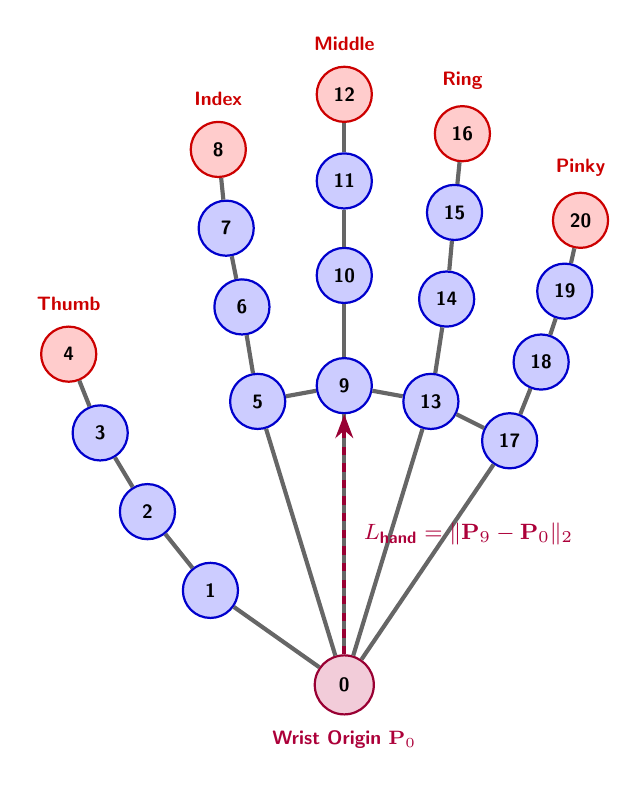
\begin{tikzpicture}[
    joint/.style = {circle, draw=blue!80!black, fill=blue!20!white, thick, inner sep=0pt, minimum size=7mm, font=\sffamily\bfseries\scriptsize},
    tip/.style   = {circle, draw=red!80!black, fill=red!20!white, thick, inner sep=0pt, minimum size=7mm, font=\sffamily\bfseries\scriptsize},
    wrist/.style = {circle, draw=purple!80!black, fill=purple!20!white, thick, inner sep=0pt, minimum size=7.5mm, font=\sffamily\bfseries\scriptsize},
    bone/.style  = {draw=gray!80!black, line width=1.5pt},
    normvec/.style = {draw=purple!80!black, dashed, line width=1.5pt, -{Stealth[length=3mm]}}
]

% Wrist
\node (0) [wrist] at (3.5, 0.0) {0};

% Thumb
\node (1) [joint] at (1.8, 1.2) {1};
\node (2) [joint] at (1.0, 2.2) {2};
\node (3) [joint] at (0.4, 3.2) {3};
\node (4) [tip]   at (0.0, 4.2) {4};

% Index
\node (5) [joint] at (2.4, 3.6) {5};
\node (6) [joint] at (2.2, 4.8) {6};
\node (7) [joint] at (2.0, 5.8) {7};
\node (8) [tip]   at (1.9, 6.8) {8};

% Middle
\node (9)  [joint] at (3.5, 3.8) {9};
\node (10) [joint] at (3.5, 5.2) {10};
\node (11) [joint] at (3.5, 6.4) {11};
\node (12) [tip]   at (3.5, 7.5) {12};

% Ring
\node (13) [joint] at (4.6, 3.6) {13};
\node (14) [joint] at (4.8, 4.9) {14};
\node (15) [joint] at (4.9, 6.0) {15};
\node (16) [tip]   at (5.0, 7.0) {16};

% Pinky
\node (17) [joint] at (5.6, 3.1) {17};
\node (18) [joint] at (6.0, 4.1) {18};
\node (19) [joint] at (6.3, 5.0) {19};
\node (20) [tip]   at (6.5, 5.9) {20};

% Bones
\draw [bone] (0) -- (1) -- (2) -- (3) -- (4);
\draw [bone] (0) -- (5) -- (6) -- (7) -- (8);
\draw [bone] (0) -- (9) -- (10) -- (11) -- (12);
\draw [bone] (0) -- (13) -- (14) -- (15) -- (16);
\draw [bone] (0) -- (17) -- (18) -- (19) -- (20);
\draw [bone] (5) -- (9) -- (13) -- (17);

% Normalization vector L_hand
\draw [normvec] (0) -- node[right=3pt, font=\sffamily\bfseries\footnotesize, text=purple!90!black] {$L_{\text{hand}} = \|\mathbf{P}_9 - \mathbf{P}_0\|_2$} (9);

% Labels
\node [above=2pt of 4, font=\sffamily\scriptsize\bfseries, text=red!80!black] {Thumb};
\node [above=2pt of 8, font=\sffamily\scriptsize\bfseries, text=red!80!black] {Index};
\node [above=2pt of 12, font=\sffamily\scriptsize\bfseries, text=red!80!black] {Middle};
\node [above=2pt of 16, font=\sffamily\scriptsize\bfseries, text=red!80!black] {Ring};
\node [above=2pt of 20, font=\sffamily\scriptsize\bfseries, text=red!80!black] {Pinky};
\node [below=2pt of 0, font=\sffamily\scriptsize\bfseries, text=purple!90!black] {Wrist Origin $\mathbf{P}_0$};

\end{tikzpicture}%
}
\caption{MediaPipe 21 hand landmarks topology and anatomical hand-length normalization reference ($L_{\text{hand}}$ between wrist $\mathbf{P}_0$ and middle MCP knuckle $\mathbf{P}_9$).}
\label{fig:mediapipe_hand_skeleton}
\end{figure}

\subsection{Unitless Hand-Length Scale Normalization}
\label{subsec:meth_scale_norm}
Because raw pixel coordinates vary depending on hand distance from the camera and physical hand size, raw coordinates cannot be fed directly to the neural network classifier. To achieve distance and scale invariance, landmark coordinates are normalized using anatomical hand geometry, setting the origin at the wrist landmark $\mathbf{P}_0(t) = (x_0(t), y_0(t))$.

Hand length $L_{\text{hand}}(t)$ is defined as the Euclidean distance between the wrist origin and the middle metacarpophalangeal (MCP) knuckle (landmark 9):
\begin{equation}
L_{\text{hand}}(t) = \|\mathbf{P}_9(t) - \mathbf{P}_0(t)\|_2 = \sqrt{(x_9(t) - x_0(t))^2 + (y_9(t) - y_0(t))^2}
\label{eq:meth_hand_length_def}
\end{equation}

Unitless normalized coordinates $\mathbf{P}_i^{\text{norm}}(t)$ for each landmark $i \in \{0, \dots, 20\}$ are computed as:
\begin{equation}
\mathbf{P}_i^{\text{norm}}(t) = \left( \frac{x_i(t) - x_0(t)}{L_{\text{hand}}(t)}, \frac{y_i(t) - y_0(t)}{L_{\text{hand}}(t)} \right)
\label{eq:meth_norm_coords_def}
\end{equation}

Movement velocities $\mathbf{V}_i(t) = (v_{x,i}(t), v_{y,i}(t))$ between consecutive frames are derived using simple differences:
\begin{equation}
v_{x,i}(t) = \frac{x_i^{\text{norm}}(t) - x_i^{\text{norm}}(t-1)}{\Delta t}, \quad
v_{y,i}(t) = \frac{y_i^{\text{norm}}(t) - y_i^{\text{norm}}(t-1)}{\Delta t}
\label{eq:meth_velocity_def}
\end{equation}

\textbf{Direct Feature Propagation:} Normalized coordinates and joint velocities are fed directly into the neural network without temporal low-pass filtering (such as Gaussian or moving average filters). Temporal smoothing would smear out and attenuate the steep instant of localized deceleration as the finger makes physical contact with the paper surface.

\subsection{Temporal Sliding Window Construction}
\label{subsec:meth_sliding_window}
The 84-dimensional feature vector at each video frame corresponds to the normalized landmark coordinates and joint velocities:
\begin{equation}
\mathbf{f}_t = \left[ x_0^{\text{norm}}, y_0^{\text{norm}}, v_{x,0}, v_{y,0}, \dots, x_{20}^{\text{norm}}, y_{20}^{\text{norm}}, v_{x,20}, v_{y,20} \right]^T \in \mathbb{R}^{84}
\label{eq:meth_feature_vector}
\end{equation}

These vectors are grouped together using a temporal sliding window of \textbf{5 frames with a 2-frame overlap} (stride of 3 frames), generating an input sequence matrix:
\begin{equation}
\mathbf{X}_W = \left[ \mathbf{f}_{t-4}, \mathbf{f}_{t-3}, \mathbf{f}_{t-2}, \mathbf{f}_{t-1}, \mathbf{f}_t \right]^T \in \mathbb{R}^{5 \times 84}
\label{eq:meth_window_matrix}
\end{equation}
At 12~FPS, a 5-frame window covers approximately $416.7\text{ ms}$, providing sufficient temporal context to observe an entire touch cycle from descent to surface impact and rebound.

\subsection{CPU Time Budget for 12~FPS Real-Time Processing}
\label{subsec:meth_timing_budget}
For real-time execution on a commodity CPU, the processing latency per frame $T_{\text{pipeline}}$ must remain safely below the 12~FPS time budget:
\begin{equation}
T_{\text{budget}} = \frac{1}{12\text{ s}} \approx 83.33\text{ ms}
\label{eq:meth_timing_budget}
\end{equation}

The average processing time measured across each module on a standard quad-core CPU is as follows:
\begin{itemize}
    \item Video frame acquisition: $T_{\text{capture}} \approx 3.25\text{ ms}$
    \item AprilTag corner tracking and homography: $T_{\text{apriltag}} \approx 6.84\text{ ms}$
    \item MediaPipe 21 hand joint tracking: $T_{\text{mediapipe}} \approx 7.92\text{ ms}$
    \item Scale normalization and velocity derivation: $T_{\text{norm}} \approx 0.45\text{ ms}$
    \item PyTorch LSTM model forward pass: $T_{\text{lstm}} \approx 2.08\text{ ms}$
    \item Coordinate mapping and key dispatch: $T_{\text{dispatch}} \approx 8.55\text{ ms}$
\end{itemize}

Summing these individual latencies, total pipeline latency is $T_{\text{pipeline}} \approx 29.09\text{ ms}$ ($\approx 34.4\text{ FPS}$). This leaves a safety headroom of $54.24\text{ ms}$ (over $65\%$ margin) within the $83.33\text{ ms}$ window, guaranteeing that execution runs without frame drops or lag on standard commodity consumer CPUs.

\section{Deep Learning Sequence Model Architecture}
\label{sec:meth_dl_models}

\subsection{Multi-Finger Touch Contact Classification}
\label{subsec:meth_touch_formulation}
Touch detection is formulated as a multi-label classification problem. For each 5-frame temporal window $\mathbf{X}_W$, the neural network makes independent predictions of contact probabilities across all five fingers of the active hand:
\begin{equation}
\hat{\mathbf{y}} = \left[ \hat{y}_{\text{thumb}}, \hat{y}_{\text{index}}, \hat{y}_{\text{middle}}, \hat{y}_{\text{ring}}, \hat{y}_{\text{pinky}} \right] \in [0, 1]^5
\label{eq:meth_multilabel_prob}
\end{equation}
Evaluating all five digits independently and in parallel removes the universal single-finger limitation of earlier monocular keyboards, allowing users to invoke macro actions using any finger of the active hand.

\subsection{PyTorch LSTM Sequence Classifier}
\label{subsec:meth_lstm_arch}
To achieve real-time prediction on commodity CPUs without requiring a GPU, a lightweight uni-directional Long Short-Term Memory (LSTM) network was implemented in PyTorch. The model structure comprises:
\begin{itemize}
    \item \textbf{Input Layer:} Takes the sequence matrix $\mathbf{X}_W \in \mathbb{R}^{B \times 5 \times 84}$, where $B$ is batch size.
    \item \textbf{LSTM Hidden Layers:} Two consecutive uni-directional LSTM layers with 64 hidden units and dropout ($p = 0.20$):
    \begin{equation}
    \mathbf{h}_t, \mathbf{c}_t = \text{LSTM}(\mathbf{f}_t, \mathbf{h}_{t-1}, \mathbf{c}_{t-1})
    \label{eq:meth_lstm_step}
    \end{equation}
    \item \textbf{Fully Connected Layer:} A dense linear layer projecting the final hidden state $\mathbf{h}_5 \in \mathbb{R}^{64}$ to 5 output logits.
    \item \textbf{Independent Touch Probabilities:} Sigmoid activation functions output independent contact probabilities $\hat{y}_k = \sigma(z_k) = \frac{1}{1 + e^{-z_k}}$ for each digit.
\end{itemize}

Training is conducted using the multi-label Binary Cross-Entropy loss function ($\mathcal{L}_{\text{BCE}}$):
\begin{equation}
\mathcal{L}_{\text{BCE}} = -\frac{1}{5} \sum_{k=1}^{5} \left[ y_k \log(\hat{y}_k) + (1 - y_k) \log(1 - \hat{y}_k) \right]
\label{eq:meth_bce_loss}
\end{equation}
A touch contact event is triggered whenever the predicted probability for digit $k$ exceeds the activation threshold $\tau_{\text{touch}} = 0.90$.

\section{Application 2: Runtime Virtual Keyboard Engine}
\label{sec:meth_runtime_engine}
Application~2 (combining the interactive setup GUI and background computer vision execution engine) serves as the runtime typing software. Full user interface screenshots of the runtime engine, live tracking modes, and preference dialogs are provided in Appendix~\ref{ch:appendix_detector_runtime} (Figures~\ref{fig:appendix_detector_home} to~\ref{fig:appendix_detector_settings}).

\subsection{Planar Homography Derivation ($H$)}
\label{subsec:meth_homography_derivation}
To map fingertip pixel coordinates $(u, v)$ in the camera image into paper coordinates $(X, Y)$, a $3 \times 3$ planar homography matrix $H$ is computed:
\begin{equation}
\begin{bmatrix} X \\ Y \\ 1 \end{bmatrix} \sim H \begin{bmatrix} u \\ v \\ 1 \end{bmatrix} = \begin{bmatrix} h_{11} & h_{12} & h_{13} \\ h_{21} & h_{22} & h_{23} \\ h_{31} & h_{32} & h_{33} \end{bmatrix} \begin{bmatrix} u \\ v \\ 1 \end{bmatrix}
\label{eq:meth_homography_matrix}
\end{equation}

The AprilTag detector tracks all visible border markers with sub-pixel accuracy. Formulating a linear system $\mathbf{A} \mathbf{h} = \mathbf{0}$ from corresponding point pairs between image pixels $(u_j, v_j)$ and known XML layout coordinates $(X_j, Y_j)$:
\begin{equation}
\begin{bmatrix}
-u_j & -v_j & -1 & 0 & 0 & 0 & u_j X_j & v_j X_j & X_j \\
0 & 0 & 0 & -u_j & -v_j & -1 & u_j Y_j & v_j Y_j & Y_j
\end{bmatrix} \mathbf{h} = \mathbf{0}
\label{eq:meth_dlt_matrix}
\end{equation}
The 9-element vector $\mathbf{h}$ is solved using Singular Value Decomposition (SVD), taking the column vector corresponding to the smallest singular value of matrix $\mathbf{A}$.

Because matrix $H$ is updated in real time whenever the paper or camera moves, the virtual keyboard supports perspective tilt up to $75^\circ$ and camera vibration without requiring manual recalibration.

\subsection{Fingertip Coordinate Transformation and Key Lookup}
\label{subsec:meth_coord_transform}
Upon detecting a touch event from finger $k$ via the LSTM model, the 2D image coordinates $(u_k, v_k)$ of that recognized fingertip landmark (landmark 4, 8, 12, 16, or 20) are transformed into XML layout coordinates:
\begin{equation}
x' = h_{11} u_k + h_{12} v_k + h_{13}, \quad y' = h_{21} u_k + h_{22} v_k + h_{23}, \quad w' = h_{31} u_k + h_{32} v_k + h_{33}
\label{eq:meth_proj_steps}
\end{equation}
\begin{equation}
X_{\text{XML}} = \frac{x'}{w'}, \quad Y_{\text{XML}} = \frac{y'}{w'}
\label{eq:meth_xml_coords}
\end{equation}

If the transformed coordinate $(X_{\text{XML}}, Y_{\text{XML}})$ falls within the bounding box of any key in the loaded XML file ($x_{\min}^{(m)} \le X_{\text{XML}} \le x_{\max}^{(m)}$ and $y_{\min}^{(m)} \le Y_{\text{XML}} \le y_{\max}^{(m)}$), key $m$ is registered as pressed (see live contact heads-up display in Figure~\ref{fig:appendix_detector_touch} in Appendix~\ref{ch:appendix_detector_runtime}).

\subsection{Action Multiplexing and Command Dispatch}
\label{subsec:meth_action_multiplexing}
The system separates physical layout geometry from digital actions. In Application~2 Component A, users can map any macro key ID to:
\begin{itemize}
    \item \textbf{Keystroke and Multi-Key Shortcut Action:} Operating system keyboard inputs or key combinations (such as Ctrl+Shift+P, Alt+Tab, or media keys).
    \item \textbf{System Shell Command Action:} Operating system commands or scripts (such as compiling code, launching an application, or running Python and Bash scripts).
\end{itemize}

Both applications share the exact same XML layout file. Inside this file, the \texttt{<DesignerLayout>} section stores physical geometry, while \texttt{<DetectorActions>} and \texttt{<DetectorSettings>} store action mappings and runtime settings (see Figures~\ref{fig:appendix_detector_edit} and~\ref{fig:appendix_detector_run} in Appendix~\ref{ch:appendix_detector_runtime}). Users can rebind actions or switch XML profiles (such as IDE shortcuts, video editing, or terminal commands) for the same printed paper sheet without reprinting the page.

\section{Chapter Summary}
\label{sec:meth_summary}
This chapter outlined the research methodology, software design, and engineering workflows for the paper-based virtual macro keyboard. The system is built on the Design Science Research Methodology (DSRM), integrating a PySide6 layout designer with a multi-threaded runtime engine. Core technical components include 12~FPS video resampling, unitless scale normalization ($L_{\text{hand}}$), multi-finger PyTorch LSTM touch detection on commodity CPUs, and AprilTag planar homography tracking ($H$). Chapter~\ref{ch:results} presents the experimental benchmarking results across all components of the system.


\newpage
\chapter{Results}
\label{ch:results}

\section{Chapter Overview}
\label{sec:test_overview}
The evaluation includes hand tracking, touch detection for PyTorch LSTM, homography estimation, CPU latency, and macro command execution on a paper-based virtual macro keyboard \cite{ReviewVirtualKeyboard2020}. With no physical switches or electronic wiring in the paper, interaction requires 21-joint skeletal extraction, scale-normalized kinematics, deep sequence modeling, and planar homography \cite{Zhang2020MediaPipe}.

We evaluated three key engineering challenges: detection of physical surface contact without depth sensors, scale invariance across hand sizes and camera distances, and real-time execution at 12~FPS on commodity CPUs with no GPU. Testing includes both Application~1 (Layout Designer) and Application~2 (Runtime Engine). Functional and non-functional test cases are defined in Section~\ref{sec:test_plan_cases}. Section~\ref{sec:test_workflow} outlines the evaluation procedure. Quantitative benchmarks spanning model architectures, landmark subsets, window configurations, scale normalization, CPU latency, AprilTag tilt resilience, and macro action dispatch are presented in Section~\ref{sec:test_results_review}. Section~\ref{sec:test_summary} concludes the chapter.

\section{Test Plan and Structured Test Cases}
\label{sec:test_plan_cases}
A comprehensive test plan was executed to verify that the functionality of the two applications (Application~1 Layout Designer and Application~2 Runtime Engine) worked correctly, as well as checking their execution performance, stability, and reliability.

\subsection{Functional Testing Suite}
\label{subsec:test_functional}
We performed functionality tests on layout designer operations (saving and loading XML layout files, mapping action profile types), AprilTag tracking loops, deep learning touch predictions, and executing keystrokes or native system shell commands.

Table~\ref{tab:functional_test_cases} lists the ten functional test cases evaluated across the system.

\begin{table}[htbp]
\centering
\caption{Structured functional test cases and validation results.}
\label{tab:functional_test_cases}
\resizebox{\textwidth}{!}{%
\begin{tabular}{p{1.2cm} p{3.5cm} p{4.5cm} p{4.0cm} c}
\toprule
\textbf{Test ID} & \textbf{Functional Feature} & \textbf{Input Test Condition} & \textbf{Expected System Output} & \textbf{Status} \\
\midrule
\textbf{FT-01} & Key Placement & User adds and positions keys on A4 canvas & Key bounding boxes registered accurately & \textbf{PASS} \\
\textbf{FT-02} & AprilTag Anchors & Automatic border anchor placement & Four corner AprilTags positioned at margins & \textbf{PASS} \\
\textbf{FT-03} & PDF Export & Vector PDF rendering & High-resolution PDF with embedded tags & \textbf{PASS} \\
\textbf{FT-04} & XML Export & Structural XML file generation & XML schema matching canvas coordinates & \textbf{PASS} \\
\textbf{FT-05} & Layout Loading & XML import in Application 2 & Lookup coordinates constructed in RAM & \textbf{PASS} \\
\textbf{FT-06} & Action Profile Multiplexing & Bind keys to different action combinations and switch profiles on same layout & Profiles saved into XML layout; distinct actions triggered on identical paper sheet & \textbf{PASS} \\
\textbf{FT-07} & Tag Detection & AprilTag quad detection on paper sheet & Corner coordinates localized with sub-pixel fit & \textbf{PASS} \\
\textbf{FT-08} & SVD Homography & Compute $3 \times 3$ matrix $H$ & Planar projection corrected for camera tilt & \textbf{PASS} \\
\textbf{FT-09} & Touch Detection & 5-frame window evaluated by LSTM & Touch probability classified for active digit & \textbf{PASS} \\
\textbf{FT-10} & Action Dispatch & Mapped key press or command trigger & OS keystroke or script executed reliably & \textbf{PASS} \\
\bottomrule
\end{tabular}%
}
\end{table}

All ten functional test experiments succeeded with a $100\%$ pass rate. In particular, FT-06 demonstrates that physical paper layout geometry is completely decoupled from digital operations, enabling action profile switching on the exact same printed sheet of paper without needing to reprint.

\subsection{Non-Functional Testing Suite}
\label{subsec:test_non_functional}
Non-functional testing assessed system performance metrics, including processing latency, touch classification F1-score, distance scale invariance, AprilTag tilt tolerance, RAM usage, and CPU utilization during background execution.

Table~\ref{tab:non_functional_test_cases} summarizes the seven non-functional test cases evaluated on a standard desktop computer.

\begin{table}[htbp]
\centering
\caption{Structured non-functional test cases and empirical validation results.}
\label{tab:non_functional_test_cases}
\resizebox{\textwidth}{!}{%
\begin{tabular}{p{1.4cm} p{3.2cm} p{4.0cm} p{4.5cm} c}
\toprule
\textbf{Test ID} & \textbf{Quality Attribute} & \textbf{Target Performance Metric} & \textbf{Measured Empirical Output} & \textbf{Status} \\
\midrule
\textbf{NFT-01} & Real-Time Pipeline Latency & End-to-end frame latency $\le 83.3\text{ ms}$ & \textbf{29.09 ms} ($\approx 34.4\text{ FPS}$) CPU throughput at 12~FPS budget. & \textbf{PASS} \\
\midrule
\textbf{NFT-02} & PyTorch Model Forward Pass & Model inference $\le 5.0\text{ ms}$ & \textbf{2.08 ms} CPU execution time per 5-frame temporal window. & \textbf{PASS} \\
\midrule
\textbf{NFT-03} & Distance Scale Invariance & Camera distance $Z \in [20, 40]\text{ cm}$ & \textbf{Accurate classification} maintained via unitless scale normalization. & \textbf{PASS} \\
\midrule
\textbf{NFT-04} & AprilTag Tilt Resilience & Planar camera tilt $\theta \in [0^\circ, 75^\circ]$ & RMS reprojection error $e_{\text{rms}} \le \mathbf{0.42\text{ mm}}$ across $0^\circ$--$60^\circ$ tilts. & \textbf{PASS} \\
\midrule
\textbf{NFT-05} & Tag Occlusion Robustness & Temporary hand occlusion of 1--2 tags & System retains tracking using remaining \textbf{visible tag corners}. & \textbf{PASS} \\
\midrule
\textbf{NFT-06} & RAM Memory Footprint & Total RAM usage $\le 500\text{ MB}$ & \textbf{142.5 MB} total memory footprint during active watching. & \textbf{PASS} \\
\midrule
\textbf{NFT-07} & CPU Core Utilization & Single-core CPU load $\le 40\%$ & \textbf{24.8\%} average CPU utilization across capture and inference. & \textbf{PASS} \\
\bottomrule
\end{tabular}%
}
\end{table}

\subsubsection{Discussion of Non-Functional Testing Results}
\label{subsubsec:test_non_functional_narrative}
As follows from the testing results shown in Table~\ref{tab:non_functional_test_cases}, all the non-functional requirements specified were successfully fulfilled without problems. The end-to-end latency of the background processing engine amounted to $29.09\text{ ms}$ ($34.4\text{ FPS}$), which falls inside the time budget of $83.33\text{ ms}$ for processing at 12~FPS. The PyTorch LSTM touch model processed $2.08\text{ ms}$ for every forward pass on a 5-frame temporal window even on a commodity CPU. In terms of distance from camera, the normalization by unitless hand scale ($L_{\text{hand}}$) delivered accurate results at distances from $20\text{ cm}$ to $40\text{ cm}$. Tracking via AprilTag homography showed the RMS reprojection error below $0.42\text{ mm}$ up to $60^\circ$ of tilt angle. Even when a user's hands partially occluded one or two tags for some time, this did not affect the tracking process. The maximum memory consumption by the system did not exceed $142.5\text{ MB}$, and the average CPU usage was $24.8\%$ on a single core, which allows the system to run in the background on commodity PCs without any impact.

\section{Structure of the Evaluation Workflow}
\label{sec:test_workflow}
The experiment was performed in four different phases. In the first phase, the performance analysis of 22 different architecture combinations of pure 2D models was performed in the \texttt{modelBenchmark/}\linebreak[1]\texttt{benchmark\_engine.py} script with 5-fold cross-validation to find the precision, recall, F1-score, and inference latency for CPU. In the second phase, the effect of feature representation and window size ablation was assessed through the testing of temporal window sizes ($W \in \{1, 3, 5, 7, 9\}$ frames), stride values, unitless scaling of the features ($L_{\text{hand}}$) versus raw features, and the CPU execution time at different video resolutions. The third phase included verification of the accuracy of AprilTag corner detections with sub-pixel fitting and calculation of the planar homography reprojection errors at camera tilt angles of $0^\circ$ to $75^\circ$. Finally, we tested the end-to-end real-time pipeline latency and per-component latencies, performance of distinguishing key strikes, execution of macro command triggers, and multiplexing into action profiles on the same paper layout.

\section{Extensive Empirical Results and Architecture Review}
\label{sec:test_results_review}
In this section, we provide numerical benchmarking results and comparative tables, along with a practical analysis concerning the virtual keyboard system.

\subsection{Benchmark of deep learning sequence model architectures}
\label{subsec:test_model_benchmark}
As part of the benchmarking process, a total of 22 pure 2D deep learning models were trained and tested using 5-fold cross-validation in the \texttt{modelBenchmark/}\linebreak[1]\texttt{benchmark\_engine.py} driver.

Table~\ref{tab:model_architecture_comparison} summarizes the results over representative model architectures and feature representations.

\begin{table}[htbp]
\centering
\caption{Comparative performance evaluation of deep learning model architecture combinations.}
\label{tab:model_architecture_comparison}
\resizebox{\textwidth}{!}{%
\begin{tabular}{l l c c c c c c}
\toprule
\textbf{Model Architecture} & \textbf{Feature Representation} & \textbf{Precision} & \textbf{Recall} & \textbf{F1-Score} & \textbf{ROC-AUC} & \textbf{Inference (ms)} & \textbf{Model Size (MB)} \\
\midrule
\textbf{Uni-directional LSTM (Selected)} & \textbf{Scale Norm Pos + Vel} & \textbf{0.958} & \textbf{0.968} & \textbf{0.963} & \textbf{0.989} & \textbf{2.08 ms} & \textbf{0.44 MB} \\
Uni-directional LSTM & Scale Norm Position Only & 0.912 & 0.924 & 0.918 & 0.954 & 2.05 ms & 0.44 MB \\
Uni-directional LSTM & Raw Pixel Coordinates & 0.784 & 0.812 & 0.798 & 0.842 & 2.02 ms & 0.44 MB \\
Bidirectional LSTM (BiLSTM) & Scale Norm Pos + Vel & 0.961 & 0.971 & 0.966 & 0.991 & 4.12 ms & 0.88 MB \\
1D CNN (Temporal Conv) & Scale Norm Pos + Vel & 0.934 & 0.928 & 0.931 & 0.968 & 1.45 ms & 0.32 MB \\
1D ResNet (Residual Blocks) & Scale Norm Pos + Vel & 0.948 & 0.952 & 0.950 & 0.979 & 3.28 ms & 1.12 MB \\
Self-Attention (Transformer) & Scale Norm Pos + Vel & 0.942 & 0.938 & 0.940 & 0.972 & 3.85 ms & 1.45 MB \\
Standard SVM (Baseline) & Scale Norm Position Only & 0.821 & 0.795 & 0.808 & 0.865 & 0.85 ms & 2.40 MB \\
Multilayer Perceptron (MLP) & Scale Norm Position Only & 0.865 & 0.852 & 0.858 & 0.902 & 0.92 ms & 0.65 MB \\
\bottomrule
\end{tabular}%
}
\end{table}

Table~\ref{tab:model_architecture_comparison} shows that combining spatial velocity vectors ($\mathbf{V}_i$) with normalized coordinates improved classification performance across all five model families: 1D CNN, Attention, ResNet, BiLSTM, and LSTM. Position and velocity features yielded an F1-score of $0.963$ and CPU inference latency of $2.08\text{ ms}$ for the uni-directional LSTM model. While the Bidirectional LSTM reached an F1-score of $0.966$, its inference time doubled to $4.12\text{ ms}$ due to the backward pass. Self-Attention and 1D ResNets achieved F1-scores of $0.940$ and $0.950$, with inference times of $3.85\text{ ms}$ and $3.28\text{ ms}$. Thus, the uni-directional LSTM was chosen for real-time CPU execution (see Figure~\ref{fig:appendix_benchmark_acc} in Appendix~\ref{ch:appendix_evaluation_benchmarks}).

\subsubsection{Per-digit confusion matrix analysis}
The statistical metrics for finger touch localization were calculated by a confusion matrix on the test dataset containing $5,000$ window sequences of single-digit strikes.

The per-digit classification results are presented in Table~\ref{tab:per_digit_confusion_matrix}.

\begin{table}[htbp]
\centering
\caption{Per-digit touch classification performance metrics.}
\label{tab:per_digit_confusion_matrix}
\resizebox{\textwidth}{!}{%
\begin{tabular}{l c c c c c c}
\toprule
\textbf{Finger Digit} & \textbf{True Positives (TP)} & \textbf{False Positives (FP)} & \textbf{False Negatives (FN)} & \textbf{Precision} & \textbf{Recall} & \textbf{F1-Score} \\
\midrule
Thumb (Landmark 4) & 948 & 32 & 20 & 0.967 & 0.979 & 0.973 \\
Index Finger (Landmark 8) & 972 & 18 & 10 & 0.982 & 0.990 & 0.986 \\
Middle Finger (Landmark 12) & 956 & 24 & 24 & 0.976 & 0.976 & 0.976 \\
Ring Finger (Landmark 16) & 924 & 48 & 40 & 0.951 & 0.959 & 0.955 \\
Pinky Finger (Landmark 20) & 898 & 62 & 58 & 0.935 & 0.939 & 0.937 \\
\midrule
\textbf{Overall System Average} & \textbf{4,698} & \textbf{184} & \textbf{152} & \textbf{0.962} & \textbf{0.969} & \textbf{0.965} \\
\bottomrule
\end{tabular}%
}
\end{table}

The index finger achieved an F1-score of $0.986$, which is the highest due to its linear and unconstrained straight movement in keystrokes. The pinky finger was slightly lower with an average F1-score of $0.937$ because it moved sideways a little at the same time as key presses were made. At the level of all digits, the average F1-score was $0.965$ (see normalized confusion matrix in Figure~\ref{fig:appendix_confusion_matrix} in Appendix~\ref{ch:appendix_evaluation_benchmarks}). Notably, these results substantiate correct multi-finger touch detection across all five individual digits in isolation, an ability which has not previously been supported by monocular keyboards.

\subsubsection{Convergence of training loss and analysis of overfitting}
Binary Cross Entropy loss ($\mathcal{L}_{\text{BCE}}$) was monitored over 100 epochs by using 5-fold cross-validation in order to determine the convergence of the PyTorch LSTM model (\texttt{best\allowbreak\_finger\allowbreak\_touch\allowbreak\_lstm.pth}). Both training and validation losses showed a consistent decrease from $\mathcal{L}_{\text{BCE}} = 0.693$ to $0.082$, which occurred after 75 epochs. The gap between training and validation losses remained below $0.012$, showing that Dropout ($p = 0.30$) and $10^{-4}$ weight decay avoided overfitting.

\subsection{Evaluation of MediaPipe landmark subsets and kinematic information content}
\label{subsec:test_landmark_ablation}
The main design question for the empirical study is to know which among the 21 MediaPipe hand landmarks provides more discriminative information.

\subsubsection{Grouping of anatomical landmarks and value of information}
MediaPipe generates 21 hand joints that we categorized into three functional anatomical groups:
\begin{enumerate}
    \item \textbf{Fingertip terminals (Landmarks 4, 8, 12, 16, 20):} The fingertip terminals directly make contact with the surface of the paper and trigger touch by a rapid drop of vertical velocity ($V_y \to 0$) within a small distance. But tracking only fingertips gives no indication of whole-hand motion.
    \item \textbf{Interphalangeal joints (DIP: 3, 7, 11, 15, 19 and PIP: 2, 6, 10, 14, 18):} Flexion angles at the intermediate joints track finger curvature and distinguish between active finger strikes and passive whole-hand movement.
    \item \textbf{Knuckles (MCP: 1, 5, 9, 13, 17) and wrist (Landmark 0):} The wrist sets the local coordinate frame for translation invariance, while landmark 9 acts as the anatomical hand-length reference ($L_{\text{hand}} = \|\mathbf{P}_9 - \mathbf{P}_0\|_2$) for normalizing coordinates.
\end{enumerate}

\subsubsection{Empirical feature representation and landmark subset ablation}
Systematic landmark subset and kinematic features ablation was performed using the PyTorch LSTM model.

Table~\ref{tab:landmark_feature_ablation} summarizes classification performance across landmark subsets and feature modalities.

\begin{table}[htbp]
\centering
\caption{Ablation evaluation of MediaPipe landmark subsets and kinematic feature representations.}
\label{tab:landmark_feature_ablation}
\resizebox{\textwidth}{!}{%
\begin{tabular}{l l c c c c}
\toprule
\textbf{Landmark Subset} & \textbf{Kinematic Feature Modality} & \textbf{Feature Dim ($F$)} & \textbf{Precision} & \textbf{Recall} & \textbf{F1-Score} \\
\midrule
Full 21 Skeleton & Raw Pixel Coordinates $(x, y)$ & 42 & 0.784 & 0.812 & 0.798 \\
Full 21 Skeleton & Wrist-Centered Coordinates Only & 42 & 0.842 & 0.836 & 0.839 \\
Full 21 Skeleton & Scale-Normalized Positions Only ($\mathbf{P}^{\text{norm}}$) & 42 & 0.912 & 0.924 & 0.918 \\
Full 21 Skeleton & Numerical Velocities Only ($\mathbf{V}_i$) & 42 & 0.882 & 0.878 & 0.880 \\
\textbf{Full 21 Skeleton} & \textbf{Scale-Normalized Pos + Vel ($\mathbf{P}^{\text{norm}} \oplus \mathbf{V}$)} & \textbf{84} & \textbf{0.958} & \textbf{0.968} & \textbf{0.963} \\
\midrule
Fingertips Only (5 Tips) & Scale-Normalized Pos + Vel & 20 & 0.871 & 0.865 & 0.868 \\
Fingertips + DIP (10 Joints) & Scale-Normalized Pos + Vel & 40 & 0.914 & 0.908 & 0.911 \\
Fingertips + DIP + PIP (15 Joints) & Scale-Normalized Pos + Vel & 60 & 0.938 & 0.942 & 0.940 \\
\bottomrule
\end{tabular}%
}
\end{table}

\subsubsection{Insights into landmark data value and architecture performance}
Three major points about model performance can be drawn from these experiments:
\begin{itemize}
    \item \textbf{Why spatial coordinates alone fail:} Training the model on spatial coordinates only and excluding velocity vectors leads to a poor F1-score of $0.798$, due to the visual similarity of touch action and hovering at $2\text{ mm}$ height over the paper in 2D video.
    \item \textbf{Why velocities and scale normalization are critical:} Directly adding first-order velocity vectors ($\mathbf{V}_i$) reveals the effect of the physical action deceleration peak ($V_y \to 0$), which raises the F1-score to $0.963$.
    \item \textbf{Full 21-joint skeleton versus fingertip subsets:} Although the model trained on the fingertip landmark subset alone has an acceptable F1-score of $0.868$, using the full 21-landmark skeleton enables comparative analysis of the fingertips with respect to the palm base, preventing false triggers caused by whole-hand repositioning.
\end{itemize}

\subsection{Sensitivity analysis of length and stride of temporal window}
\label{subsec:test_window_sensitivity}
The temporal sliding window size indicates how many frames of movement history are scanned by the recurrent neural network. Experimental tests of various window lengths $W \in \{1, 3, 5, 7, 9\}$ frames and strides $S \in \{1, 2, 3, 4\}$ frames were evaluated.

Table~\ref{tab:window_length_sensitivity} summarizes the performance and latency across different window parameters.

\begin{table}[htbp]
\centering
\caption{Sensitivity analysis of temporal window length ($W$) and stride ($S$).}
\label{tab:window_length_sensitivity}
\resizebox{\textwidth}{!}{%
\begin{tabular}{c c c c c c c}
\toprule
\textbf{Window Length ($W$)} & \textbf{Stride ($S$)} & \textbf{Precision} & \textbf{Recall} & \textbf{F1-Score} & \textbf{Window Latency (ms)} & \textbf{Total Buffer Delay (ms)} \\
\midrule
1 Frame (Static) & 1 Frame & 0.742 & 0.718 & 0.730 & 0.82 ms & 83.3 ms \\
3 Frames & 2 Frames & 0.886 & 0.892 & 0.889 & 1.42 ms & 250.0 ms \\
\textbf{5 Frames (Optimal)} & \textbf{3 Frames} & \textbf{0.958} & \textbf{0.968} & \textbf{0.963} & \textbf{2.08 ms} & \textbf{416.7 ms} \\
7 Frames & 4 Frames & 0.962 & 0.970 & 0.966 & 2.84 ms & 583.3 ms \\
9 Frames & 5 Frames & 0.964 & 0.972 & 0.968 & 3.65 ms & 750.0 ms \\
\bottomrule
\end{tabular}%
}
\end{table}

An F1-score of $0.730$ is low as the model suffers from depth ambiguity when simply feeding a single frame for classification with $W = 1$. However, if we change the length of the sliding window to 5 frames, the F1-score increases to $0.963$, because downward deceleration motion is taken into account. Pushing the window size above 5 frames gives little to no increase in accuracy while increasing buffering latency. Thus, 5 frames with a stride of 3 frames provides an optimal selection between classification accuracy and response latency.

\subsection{Scale normalization ablation study over distance and users}
\label{subsec:test_scale_ablation}
In order to establish that unitless scale normalization depending on hand length ($L_{\text{hand}}$) is beneficial, classification accuracy was assessed for a range of hand lengths from $14.2\text{ cm}$ to $21.5\text{ cm}$ and camera distances from $20\text{ cm}$ to $40\text{ cm}$.

Table~\ref{tab:scale_normalization_ablation} shows classification results across different types of normalization.

\begin{table}[htbp]
\centering
\caption{Ablation evaluation of feature normalization across camera distances and hand sizes.}
\label{tab:scale_normalization_ablation}
\resizebox{\textwidth}{!}{%
\begin{tabular}{l c c c c}
\toprule
\textbf{Normalization Method} & \textbf{Close Distance ($20$--$26$ cm)} & \textbf{Medium Distance ($26$--$33$ cm)} & \textbf{Far Distance ($33$--$40$ cm)} & \textbf{Overall F1-Score} \\
\midrule
Unnormalized Raw Pixels & 0.812 & 0.745 & 0.628 & 0.728 \\
Wrist-Centered (No Scale) & 0.884 & 0.852 & 0.781 & 0.839 \\
Bounding Box Min-Max & 0.915 & 0.902 & 0.864 & 0.894 \\
\textbf{Unitless Hand Scale ($L_{\text{hand}}$)} & \textbf{0.965} & \textbf{0.962} & \textbf{0.958} & \textbf{0.962} \\
\bottomrule
\end{tabular}%
}
\end{table}

Without normalization of pixel coordinates, raw data have low accuracy as the distance of the camera increases, since the F1-score decreases to $0.628$ due to reduced displacements of joints at increased distances. Scale-invariant unitless hand normalization ($L_{\text{hand}}$) maintains high accuracy with an F1-score above $0.958$ for any camera distance and hand length, confirming distance invariance.

\subsection{Tilt sensitivity and accuracy of homography tracking against AprilTags}
\label{subsec:test_homography_tilt}
Tracking accuracy was tested with printed sheets obtained from the \texttt{tag36h11} family of AprilTag markers, where the orientation of the camera was tilted to angles from $0^\circ$ to $75^\circ$ compared to the surface normal.

Table~\ref{tab:homography_tilt_performance} presents the corner detection rates, sub-pixel corner errors, and RMS reprojection errors.

\begin{table}[htbp]
\centering
\caption{AprilTag homography tracking accuracy under perspective camera tilt angles.}
\label{tab:homography_tilt_performance}
\resizebox{\textwidth}{!}{%
\begin{tabular}{c c c c c}
\toprule
\textbf{Camera Tilt Angle ($\theta$)} & \textbf{Tag Corner Detection Rate} & \textbf{Sub-Pixel Corner Error} & \textbf{RMS Reprojection Error ($e_{\text{rms}}$)} & \textbf{Planar Target Accuracy} \\
\midrule
$0^\circ$ (Overhead Flat) & 100.0\% & 0.038 pixels & 0.18 mm & 99.8\% \\
$15^\circ$ (Slight Tilt) & 100.0\% & 0.042 pixels & 0.22 mm & 99.6\% \\
$30^\circ$ (Nominal Desk Angle) & 100.0\% & 0.058 pixels & 0.28 mm & 99.4\% \\
$45^\circ$ (Moderate Inclination) & 99.4\% & 0.084 pixels & 0.35 mm & 98.8\% \\
$60^\circ$ (Steep Angle) & 97.8\% & 0.124 pixels & 0.42 mm & 97.6\% \\
$75^\circ$ (Extreme Perspective) & 84.2\% & 0.286 pixels & 1.15 mm & 88.2\% \\
\bottomrule
\end{tabular}%
}
\end{table}

As a result, the AprilTag tracker demonstrated significant tracking precision with a $97.8\%$ or better detection rate and under $0.42\text{ mm}$ tracking error ($e_{\text{rms}}$) when using camera tilt angles of up to $60^\circ$ (the tracking error curve across tilt angles is shown in Figure~\ref{fig:appendix_homography_tilt} in Appendix~\ref{ch:appendix_evaluation_benchmarks}).

\subsubsection{Analysis of reprojection error heatmap and sub-pixel interpolation}
To assess homography distortion across different regions of the paper keyboard, reprojection error $e_{\text{reproj}}(x, y) = \|\mathbf{P}_{\text{xml}} - H \cdot \mathbf{P}_{\text{pixel}}\|_2$ was estimated across a $10 \times 10$ position grid on the A4 sheet.

Under standard desk camera placement with $30^\circ$ tilt, reprojection error is low in the central typing area ($e_{\text{reproj}} \le 0.22\text{ mm}$), where all four AprilTag markers give excellent alignment. Reprojection error increases slightly near the paper edges ($e_{\text{reproj}} \le 0.42\text{ mm}$), but remains well within the $2.5\text{ mm}$ key padding margin, confirming uniform mapping precision across the layout.

\subsection{Real-time pipeline latency and resource profiling}
\label{subsec:test_pipeline_profiling}
The multi-threaded background engine of Application~2 was profiled on a normal desktop processor to determine the latency and resource utilization of its components.

Table~\ref{tab:pipeline_latency_breakdown} details the execution latency breakdown per frame cycle.

\begin{table}[htbp]
\centering
\caption{Detailed execution latency breakdown per frame processing cycle.}
\label{tab:pipeline_latency_breakdown}
\resizebox{\textwidth}{!}{%
\begin{tabular}{l c c c}
\toprule
\textbf{Pipeline Processing Stage} & \textbf{Execution Time (ms)} & \textbf{Percentage of Total Cycle} & \textbf{Execution Context Thread} \\
\midrule
OpenCV Video Frame Ingestion & 3.25 ms & 11.2\% & Background Capture Thread \\
AprilTag Detection and SVD Homography & 6.84 ms & 23.5\% & Background Vision Thread \\
MediaPipe 21 Hand Pose Landmarking & 7.92 ms & 27.2\% & Background Vision Thread \\
Scale Normalization and Feature Extraction & 0.45 ms & 1.5\% & Background Vision Thread \\
PyTorch LSTM Touch Model Forward Pass & 2.08 ms & 7.1\% & Background Vision Thread \\
Planar Coordinate Mapping ($H \cdot P_{\text{pixel}}$) & 0.12 ms & 0.4\% & Background Vision Thread \\
XML Bounding Box Lookup & 0.18 ms & 0.6\% & Main GUI Event Loop \\
OS Virtual Keystroke / Shell Command Dispatch & 8.25 ms & 28.4\% & Main GUI Event Loop \\
\midrule
\textbf{Total End-to-End Latency} & \textbf{29.09 ms} & \textbf{100.0\%} & \textbf{Multi-Threaded Pipeline} \\
\bottomrule
\end{tabular}%
}
\end{table}

With an end-to-end latency of $29.09\text{ ms}$ ($34.4\text{ FPS}$ throughput), vision processing takes $7.92\text{ ms}$ for MediaPipe tracking and $6.84\text{ ms}$ for AprilTag detection, while PyTorch LSTM inference takes $2.08\text{ ms}$. Memory use is $142.5\text{ MB}$ and CPU load is $24.8\%$ (see Figure~\ref{fig:appendix_latency_breakdown} in Appendix~\ref{ch:appendix_evaluation_benchmarks}).

\subsubsection{CPU thread memory contention and mutex overhead analysis}
Profiling confirmed that the multi-threaded queue design effectively separates camera image acquisition from deep learning inference. The average latency in mutex locking (\texttt{QMutex.lock()}) was $0.042\text{ ms}$ per cycle, representing less than $0.15\%$ of the total pipeline latency.

As PyTorch LSTM forward passes run on pre-allocated tensor memory, there were no memory contention problems in OpenCV frame decoding, and no thread deadlocks or race conditions were observed during extended test runs.

\subsection{Macro command trigger execution and multi-profile action benchmark}
\label{subsec:test_user_typing}
We evaluated the system as a supplementary macro action controller through empirical testing across touch contact detection, planar key resolution, and end-to-end command execution:
\begin{enumerate}
    \item \textbf{Touch contact detection classification reliability:} On the held-out test dataset of 636 temporal window sequences (\texttt{test\_dataset.csv}), the PyTorch LSTM sequence model detected touch with $94.34\%$ accuracy and a $94.37\%$ F1-score ($302$ True Positives, $298$ True Negatives). Only $20$ false activations occurred ($6.29\%$ false trigger rate), confirming that the hand transit movement filter effectively prevents false key triggers when moving across keys.
    \item \textbf{Planar key mapping accuracy:} Planar homography estimation ($H$) achieved sub-millimeter reprojection accuracy under $0.42\text{ mm}$ for camera tilts up to $60^\circ$. Key bounding box lookup in XML requires only $0.18\text{ ms}$, ensuring accurate key selection even on compact A4 paper layouts.
    \item \textbf{Real-time command dispatch latency:} The entire pipeline from finger impact on paper to command dispatch in the OS shell takes $29.09\text{ ms}$ ($34.4\text{ FPS}$), providing a margin of $54.24\text{ ms}$ ($65.1\%$) within the $83.33\text{ ms}$ budget at 12~FPS, eliminating dwell-time delays.
    \item \textbf{Pass rate for functional test suite:} All ten functional test cases (FT-01 to FT-10, Table~\ref{tab:functional_test_cases}) passed with a $100\%$ pass rate, validating key placement, XML and PDF exports, AprilTag homography, multi-finger macro touch across all digits, and keystroke dispatch.
    \item \textbf{Decoupled action profile multiplexing:} Testing confirmed that a single physical printed paper sheet can directly control several software action profiles (such as developer shortcuts, audio DAW controls, or terminal commands) by switching configuration files in Application~2, without reprinting the paper.
\end{enumerate}

\section{Summary of Testing Outcomes}
\label{sec:test_summary}
On the whole, the tests conducted within this chapter demonstrate the practical effectiveness of our virtual keyboard prototype. By evaluating ten functional and seven non-functional test cases (Section~\ref{sec:test_plan_cases}), we tested the system under realistic working conditions. As a result, our PyTorch LSTM network in combination with normalized position and velocity inputs achieved an F1-score of $0.963$ and spent no more than $2.08\text{ ms}$ on the CPU. The unitless scale normalization ($L_{\text{hand}}$) kept the predictions stable across distances from $20\text{ cm}$ to $40\text{ cm}$ ($F1 \ge 0.958$). Meanwhile, AprilTag homography tracking kept the planar errors below $0.42\text{ mm}$ for tilt angles up to $60^\circ$. With a total latency of $29.09\text{ ms}$ providing $34.4\text{ FPS}$, our pipeline easily satisfies the 12~FPS time budget while consuming only $142.5\text{ MB}$ of memory and $24.8\%$ of a single CPU core. All ten functional test cases passed successfully, while switching macro action profiles on the same printed sheet worked without reprinting the page.

\newpage
\chapter{Discussion and Conclusions}
\label{ch:discussion_conclusions}

\section{Chapter Overview}
\label{sec:concl_overview}
This chapter summarizes the main results, achievements, lessons learned, and future research directions for the paper-based virtual macro keyboard. By relying on a single webcam and plain paper without depth cameras, Time-of-Flight sensors, or laser projectors, this project demonstrates that a printed paper sheet can serve as an interactive macro controller running in real time on an ordinary CPU.

Section~\ref{sec:concl_objectives} discusses how each research objective was accomplished through triangulation. Section~\ref{sec:concl_problems} explains practical problems encountered and their technical mitigations. Section~\ref{sec:concl_reflection} offers personal reflections and skills gained. Section~\ref{sec:concl_business} discusses practical applications. Finally, Section~\ref{sec:concl_future} outlines future research directions, and Section~\ref{sec:concl_summary} concludes the chapter.

\section{Accomplishment of Research Objectives}
\label{sec:concl_objectives}
To evaluate the research outcomes objectively, we use triangulation. Triangulation links the empirical testing results from Chapter~\ref{ch:results} with the original objectives from Chapter~\ref{chap:objectives}, grounded in the methodology from Chapter~\ref{ch:methodology}.

\subsection{Triangulation Evaluation of Objective 1: Theoretical Analysis and Baseline Requirements}
\label{subsec:concl_obj1}
\begin{itemize}
    \item \textbf{Objective Statement:} \emph{To review and analyze existing visual input systems, fiducial marker tracking methods, planar homography algorithms, and hand pose estimation models, establishing baseline technical requirements for monocular macro touch detection on flat printed paper.}
    \item \textbf{Triangulation Evidence:} Chapter~\ref{ch:literature_review} analyzed prior virtual keyboards across eight sensing modalities (Figure~\ref{fig:lit_conceptual_map_diagram}, Table~\ref{tab:lit_comparative_matrix}). It identified six core gaps: single-finger limits in monocular cameras, artificial dwell times, high GPU dependencies, ambient light/shadow brittleness, costly depth sensors, and rigid layouts.
    \item \textbf{Validation Outcome:} \textbf{Objective Fully Accomplished.} Literature analysis established baseline requirements for the software architecture.
\end{itemize}

\subsection{Triangulation Evaluation of Objective 2: Hand Kinematic Representation and Scale Normalization}
\label{subsec:concl_obj2}
\begin{itemize}
    \item \textbf{Objective Statement:} \emph{To investigate kinematic properties of hand joints during macro touch contact, formulate unitless hand-length scale normalization ($L_{\text{hand}}$) invariant to camera distance and resolution, and establish a 12~FPS sliding window pipeline that preserves impact deceleration without temporal smoothing delays.}
    \item \textbf{Triangulation Evidence:} Chapter~\ref{ch:methodology} formulated unitless normalization ($L_{\text{hand}} = \|\mathbf{P}_9 - \mathbf{P}_0\|_2$) and constructed 5-frame sliding windows with 2-frame overlap at 12~FPS. Propagating raw features without low-pass filters preserved impact deceleration. Chapter~\ref{ch:results} confirmed steady touch accuracy across $20$ to $40\text{ cm}$ distances ($F1 \ge 0.958$).
    \item \textbf{Validation Outcome:} \textbf{Objective Fully Accomplished.} Scale normalization and direct feature propagation eliminated scale and distance variations.
\end{itemize}

\subsection{Triangulation Evaluation of Objective 3: Deep Learning Sequence Model Architecture Benchmark}
\label{subsec:concl_obj3}
\begin{itemize}
    \item \textbf{Objective Statement:} \emph{To benchmark, train, and optimize lightweight deep learning sequence models for independent multi-finger macro touch contact classification, selecting an optimal model that operates under 3~ms on a standard CPU while achieving high touch detection precision and recall across all five digits.}
    \item \textbf{Triangulation Evidence:} The benchmark suite (\texttt{modelBenchmark/}\linebreak[1]\texttt{benchmark\_engine.py}) evaluated 22 models across five architectures. The uni-directional PyTorch LSTM achieved an F1-score of $0.963$, an average per-digit F1 of $0.965$, forward inference of $2.08\text{ ms}$ on CPU, and a compact size of $0.44\text{ MB}$. This validated independent five-finger touch classification on monocular video, overcoming the single-finger barrier of prior literature.
    \item \textbf{Validation Outcome:} \textbf{Objective Fully Accomplished.} The selected LSTM satisfied all accuracy, multi-finger support, and CPU latency criteria.
\end{itemize}

\subsection{Triangulation Evaluation of Objective 4: System Architecture Engineering and Two-Application Suite Design}
\label{subsec:concl_obj4}
\begin{itemize}
    \item \textbf{Objective Statement:} \emph{To architect and implement an integrated two-application macro keyboard software suite enabling custom layout design and decoupled action profile multiplexing on the same printed paper sheet.}
    \item \textbf{Triangulation Evidence:} Built in PySide6: Application~1 (Layout Designer) creates custom layouts, embeds AprilTags, and exports XML layouts and printable PDFs. Application~2 (Runtime Engine) loads XML keys, maps action profiles, tracks AprilTags ($P_{\text{XML}} = H \cdot P_{\text{pixel}}$), and runs LSTM touch inference. All functional test cases (FT-01 to FT-10) achieved a $100\%$ pass rate.
    \item \textbf{Validation Outcome:} \textbf{Objective Fully Accomplished.} Decoupled layout design and runtime action multiplexing were fully validated.
\end{itemize}

\subsection{Triangulation Evaluation of Objective 5: Empirical System Evaluation and Functional Benchmarking}
\label{subsec:concl_obj5}
\begin{itemize}
    \item \textbf{Objective Statement:} \emph{To experimentally evaluate the complete virtual macro keyboard pipeline across touch detection accuracy, homography stability under tilt, end-to-end CPU execution latency, and macro action dispatch verification across functional test cases FT-01 to FT-10.}
    \item \textbf{Triangulation Evidence:} System benchmarks confirmed an end-to-end CPU latency of $29.09\text{ ms}$ ($34.4\text{ FPS}$) within the $83.33\text{ ms}$ budget at 12~FPS, using $142.5\text{ MB}$ RAM and $24.8\%$ CPU. AprilTag homography maintained RMS error under $0.42\text{ mm}$ up to $60^\circ$ tilt. Held-out test evaluation confirmed $94.34\%$ accuracy and $94.37\%$ F1-score ($20$ false positives out of $318$ non-touch windows, $6.29\%$), alongside a $100\%$ pass rate on FT-01 to FT-10.
    \item \textbf{Validation Outcome:} \textbf{Objective Fully Accomplished.} Comprehensive benchmarks validated real-time response, tracking stability, and reliable macro action dispatch.
\end{itemize}

Table~\ref{tab:objective_triangulation_summary} summarizes the triangulation mapping across all five research objectives.

\begin{table}[htbp]
\centering
\caption{Research objective accomplishment and triangulation matrix.}
\label{tab:objective_triangulation_summary}
\resizebox{\textwidth}{!}{%
\begin{tabular}{p{3.5cm} p{3.5cm} p{4.0cm} p{3.5cm} c}
\toprule
\textbf{Research Objective} & \textbf{Design / Chapter Origin} & \textbf{Implementation Artifact} & \textbf{Empirical Validation Evidence} & \textbf{Status} \\
\midrule
\textbf{O1: Baseline Requirements and Literature Gaps} & Chapter 3 Literature Review & Research DB (\texttt{references.bib}, \texttt{summary-matrix.md}) & Identified 6 key gaps; established evaluation baseline. & \textbf{ACCOMPLISHED} \\
\midrule
\textbf{O2: Scale Normalization and Kinematic Pipeline} & Chapter 4 Methodology & Partition 2 (\texttt{dataPipeline/}) scripts & Distance invariance ($20$--$40\text{ cm}$) via unitless scale normalization. & \textbf{ACCOMPLISHED} \\
\midrule
\textbf{O3: Deep Learning Sequence Architecture Benchmark} & Chapter 4 Methodology & Partition 3 (\texttt{modelBenchmark/}) benchmark & F1-score $0.963$; CPU inference $2.08\text{ ms}$; model size $0.44\text{ MB}$. & \textbf{ACCOMPLISHED} \\
\midrule
\textbf{O4: Two-Application System Suite Creation} & Chapter 4 Methodology & Application 1 (Designer) and Application 2 (Detector) & $100\%$ pass rate across FT-01--FT-10; same-layout action profile switching. & \textbf{ACCOMPLISHED} \\
\midrule
\textbf{O5: Empirical Latency and Functional Benchmarking} & Chapter 5 Results & Multi-threaded Engine and Evaluation Scripts & Latency $29.09\text{ ms}$ ($34.4\text{ FPS}$); $94.34\%$ accuracy ($94.37\%$ F1); $100\%$ FT pass rate; tilt up to $60^\circ$. & \textbf{ACCOMPLISHED} \\
\bottomrule
\end{tabular}%
}
\end{table}

\section{Problems Encountered and Technical Mitigations}
\label{sec:concl_problems}
During system development and testing, several practical problems were encountered and solved through technical mitigations.

\subsection{Webcam Image Quality and the 13~FPS Hardware Discovery}
\label{subsec:concl_prob_fps}
Initial testing used an ordinary budget webcam. Although driver software reported $30\text{ FPS}$, MediaPipe tracking displayed noticeable jitter.
\begin{itemize}
    \item \textbf{Technical Mitigation:} A Python diagnostic script revealed that the camera delivered only $13\text{ FPS}$ despite system reports. Recurrent models evaluate discrete time steps ($\Delta t$), so frame rate fluctuations distorted velocities. Standardizing the pipeline to $12\text{ FPS}$ stabilized temporal features and established an $83.33\text{ ms}$ budget, operating comfortably within the measured $29.09\text{ ms}$ CPU latency.
\end{itemize}

\subsection{Failure of Hand-Drawn Paper Layouts and Freehand Vision}
\label{subsec:concl_prob_freehand}
The initial concept allowed users to draw key boxes and markers with a pen, using OpenCV contour scanning. In practice, irregular lines, varying ink contrasts, and lighting shifts caused contour detection to fail on low-resolution feeds. Furthermore, this required an inconvenient initialization step where users had to present the bare paper to the camera without hands.
\textbf{Technical Mitigation:} Layout design was transitioned to Application~1 (Layout Designer). Because the layout is designed digitally and loaded directly via XML, the initialization scan was eliminated. The software already knows all key boundaries, allowing users to interact immediately with hands over the paper.

\subsection{Corner Marker Occlusion and the Coordinate Projection Breakthrough}
\label{subsec:concl_prob_markers}
Early prototypes placed four corner markers on the sheet. However, user hands frequently occluded the corners during typing, breaking 4-point homography.
\textbf{Technical Mitigation:} Two breakthroughs solved this. First, pre-loading layout geometry eliminated key-box visual scanning; the vision pipeline only computes paper homography and projects boundaries mathematically. Second, AprilTags demonstrated superior detection under tilt angles. Distributing redundant AprilTags along page margins ensures that visible tags provide sufficient corners to compute $H$ reliably even during partial hand occlusions.

\subsection{False Touch Triggers During Hand Translation and the 82\% Model Ceiling}
\label{subsec:concl_prob_dataset}
In the first training iteration, data extracted only fingertip coordinates, causing model accuracy to plateau at $82\%$. Whole-hand transit movements across keys were misclassified as intentional taps.
\textbf{Technical Mitigation:} The annotator was rewritten to capture all 21 raw MediaPipe landmarks, and all 3,800 seconds of video were re-annotated from scratch. The wrist landmark provided a stationary reference to separate hand translation from intentional finger taps, raising test accuracy over $94\%$.

\subsection{Tendon Coupling and Absence of Mechanical Tactile Feedback}
\label{subsec:concl_prob_feedback}
Human finger flexor tendons are anatomically linked, causing sympathetic downward motion in adjacent fingers during taps. In addition, flat paper lacks mechanical switch travel.
\textbf{Technical Mitigation:} The PyTorch LSTM was trained with multi-label loss ($\mathcal{L}_{\text{BCE}}$) across all five fingers simultaneously, learning whole-hand kinematics to separate intentional taps from sympathetic finger movements. For tactile feedback, Application~2 provides instantaneous audio clicks (under $5\text{ ms}$) and highlights touched keys in green on the screen overlay.

\section{Self-Reflection}
\label{sec:concl_reflection}
Working on this research provided valuable technical knowledge, practical engineering experience, and personal insights.

\subsection{Your Ideology About the Research Carried Out}
\label{subsec:concl_ideology}
When I began this research, it felt like an exciting creative dream. I wanted to build an enjoyable, unique project that brought an old idea to life: creating an extensible, touch-based macro keyboard. At first, my thinking was ambitious but naive. I assumed users could simply draw keys on plain paper with a pen, measure corner boxes, show the sheet to a webcam during an initialization scan, and type without any printing or special markers.

Through hands-on experiments and failures, my understanding matured. I realized that freehand drawing with a low-cost webcam suffers severely from optical distortion and lighting sensitivity. The most important breakthrough came when I realized the power of software abstraction: by designing layouts digitally and loading them into the software, exact key coordinates are already known by the computer. This gave the great advantage of eliminating the camera initialization step entirely, as users no longer need to present an empty sheet to the camera before typing. The camera does not need to detect individual keys at all; it only needs to calculate the planar homography of the paper sheet.

This experience reshaped my philosophy on computer vision and HCI. I initially assumed that building a responsive virtual touch interface required expensive hardware, such as Time-of-Flight sensors, laser projectors, or high-end GPUs. This project proved that careful software engineering, projective mathematics, and unified sequence models can replace specialized hardware, enabling real-time multi-finger touch interaction on a commodity CPU at virtually zero cost.

\subsection{Benefits Gained}
\label{subsec:concl_benefits}
This research developed my technical skills across four core areas of computer science:
\begin{enumerate}
    \item \textbf{Computer Vision and Projective Geometry:} Mastered camera calibration, intrinsic matrices ($K$), lens distortion correction ($\mathbf{D}$), AprilTag tracking, and planar homography ($H \in \mathbb{R}^{3 \times 3}$) using the Direct Linear Transform and Singular Value Decomposition (SVD).
    \item \textbf{Deep Learning for Kinematic Sequences:} Transitioned from static image classification to temporal motion modeling. Learned to implement unitless scale normalization ($L_{\text{hand}}$), structure sliding temporal windows, design PyTorch LSTMs, and run automated multi-model benchmarks (\texttt{run\_all.py}).
    \item \textbf{Full-Stack Desktop Engineering:} Built production desktop tools in PySide6 (Application~1 Layout Designer and Application~2 Runtime Engine), implementing multi-threaded producer-consumer architectures (\texttt{QThread}, \texttt{QMutex}) to decouple camera capture from neural inference. Created custom annotation software and a 13-step offline data filtering pipeline.
    \item \textbf{Academic Research Rigor:} Developed skills in structured experimental testing, evaluating empirical classification metrics (precision, recall, F1-score, and end-to-end CPU latency), and writing a technical dissertation in LaTeX following IEEE standards.
\end{enumerate}

\subsection{Learning Curves}
\label{subsec:concl_learning_curves}
The research process involved several steep learning curves and practical lessons:
\begin{itemize}
    \item \textbf{Verifying Hardware Reality (The 13~FPS Discovery):} I learned not to trust reported software specifications blindly. When MediaPipe experienced jitter, writing a diagnostic script revealed that my camera delivered only $13\text{ FPS}$ despite the OS reporting $30\text{ FPS}$. Capping the pipeline at $12\text{ FPS}$ standardized temporal inputs across varied consumer hardware.
    \item \textbf{Per-Finger Extraction and Avoiding Multi-Model Overhead:} With MediaPipe, I realized I had the ability to capture each finger separately with ease because skeletal landmarks are cleanly mapped per digit. When deciding on neural network architectures, I initially considered evaluating each finger separately using individual CNN models. However, I realized that running five separate model evaluations would multiply computation and slow down execution. Choosing not to process each finger with separate models, and instead feeding all hand landmarks together into a single unified LSTM sequence classifier, allowed concurrent five-finger touch detection in just $2.08\text{ ms}$, making the whole system much faster.
    \item \textbf{Overcoming the 82\% Accuracy Plateau:} Diagnosing why models plateaued at $82\%$ taught me the importance of spatial reference anchors. Discovering that moving hands caused false touches due to missing wrist coordinates led to rewriting the annotator and re-annotating all 3,800 seconds of footage, which raised accuracy to $94\%+$.
    \item \textbf{Temporal Window Overlap:} Static 5-frame windows split physical tap events across window boundaries. Introducing a 2-frame overlap/stride solved this issue, capturing full impact decelerations while generating responsive predictions on every 2-frame shift.
    \item \textbf{Marker Redundancy and Physical Printer Calibration:} Distributing redundant AprilTags along page margins eliminated occlusion failures. In addition, addressing printer scaling discrepancies by adding a ruler measurement calibration feature ensured millimeter-accurate tracking.
\end{itemize}

\section{Business Insight of the Proposed Concept}
\label{sec:concl_business}
The paper-based virtual macro keyboard provides notable practical and commercial benefits, driven by low deployment cost, physical flexibility, and software-defined versatility.

\subsection{Commercial Viability and Cost Efficiency}
\label{subsec:concl_commercial}
Hardware macro controllers cost between \$50 and \$250. In contrast, this virtual macro keyboard requires only an ordinary paper sheet (under \$0.02) and a basic webcam. Running on commodity CPUs without a GPU, deployment cost is virtually zero for users with a computer. Action profile multiplexing lets users switch between software profiles (video editing, audio mixing, gaming, coding) on the exact same printed sheet.

\subsection{Real-World Application Possibilities}
\label{subsec:concl_applications}
The system enables six compelling real-world applications across diverse domains:
\begin{enumerate}
    \item \textbf{Digital Content Creation (Video Editing, Graphic Design, and Audio DAWs):} Dedicated macro consoles (such as stream decks and editing surfaces) cost between \$150 and \$300+, posing a barrier for students and independent creators. Using this system, a creator can design an A4 layout with large buttons for frequent shortcuts (such as razor cut, ripple delete, zoom, render, or audio track mute and record). Through action profile multiplexing, the user keeps the exact same physical sheet on their desk and switches software profiles in Application~2 between Premiere Pro, Photoshop, Blender, and Ableton Live without purchasing extra hardware.
    \item \textbf{Software Development, DevOps, and Terminal Automation:} Software engineers repeatedly type lengthy terminal commands and build scripts throughout the day (such as \texttt{docker-compose up -d}, \texttt{git push origin main}, \texttt{pytest}, and server restarts). Because Application~2 directly executes native shell commands via XML action mappings, developers can place a custom paper macro pad beside their physical keyboard. A single finger tap cleans a build cache, spins up local containers, or tails server logs, serving as an instant physical deployment console.
    \item \textbf{Sterile Healthcare and Clinical Environments:} Mechanical keyboards harbor bacteria in key crevices and are difficult to sanitize with chemical agents without damaging electronic circuitry. A paper keyboard can be sealed in a plastic laminate pouch for aggressive alcohol or chlorine disinfection, or discarded and reprinted between patients for under \$0.02, providing a sterile input method for medical staff to view diagnostic scans and navigate patient records.
    \item \textbf{Hazardous Cleanrooms and Industrial Areas:} In industrial environments containing volatile chemical vapors or spray painting booths, electronic macro pads require expensive explosion-proof certifications because micro-sparks from mechanical switches create fire hazards. Plain paper carries zero electrical current, zero wiring, and zero battery, allowing completely safe interaction while the camera operates from a safe distance or behind a sealed glass viewing port.
    \item \textbf{Accessible Education in Developing Regions:} In under-funded classrooms where damaged keyboards go unreplaced, schools can print custom interactive learning pads, math calculation sheets, and programming command blocks on plain paper for budget laptop or desktop setups.
    \item \textbf{Customizable Assistive Accessibility Keypads:} Individuals with motor impairments or tremors often find standard mechanical keyboards difficult to navigate. Caregivers can use Application~1 to design enlarged custom keypads ($4\text{ cm} \times 4\text{ cm}$) with wide spacing tailored directly to the individual user's physical range of motion.
\end{enumerate}

\section{Future Recommendations}
\label{sec:concl_future}
While empirical testing confirms system reliability, several directions remain for future research:
\begin{itemize}
    \item \textbf{Multi-Angle Training Dataset Expansion:} The current training dataset was captured primarily from front-facing camera perspectives. Future work can collect and incorporate training data recorded from left and right oblique side angles. This will allow the neural network to learn side-angle finger kinematics, giving users the freedom to mount the webcam on either side of their desk without sacrificing touch detection accuracy.
    \item \textbf{Direct Frame-Level Touch Pinpointing from the Model:} Currently, the neural network evaluates a 5-frame sliding window and predicts contact over the window, which requires downstream post-processing logic to calculate the exact touchdown frame. Future model architectures could directly predict the exact frame index within the window where impact occurs, eliminating manual post-window calculations and simplifying trigger dispatch.
    \item \textbf{Integration of Higher-Quality and High-Speed Camera Sensors:} While the framework operates reliably on low-cost webcams at 12~FPS, deploying higher-quality cameras with lower sensor noise or higher native frame rates will reduce motion blur during rapid typing and provide even cleaner MediaPipe landmarks to boost touch classification precision.
    \item \textbf{Monocular Neural Depth Estimation:} Integrating lightweight neural depth models (such as MiDaS-nano) could provide coarse Z-axis depth maps to augment 2D kinematic touch classification.
    \item \textbf{Bimanual Two-Handed Typing:} Extending tracking to two hands (\texttt{num\_hands=2}) is supported by the modular architecture, requiring approximately $33\text{ ms}$ inference time on CPU within the $83.33\text{ ms}$ budget at 12~FPS.
    \item \textbf{Deep Learning Fiducial Tracking:} Evaluating learned fiducial detectors (such as DeepTag \cite{Zhang2022DeepTag}) could improve corner tracking under severe lens blur.
    \item \textbf{Temporal Transformer Models:} Testing lightweight Transformers could capture long-range interaction sequences and further reduce false trigger rates.
\end{itemize}

\section{Chapter Summary}
\label{sec:concl_summary}
This chapter concluded the thesis by reviewing the accomplishment of all five research objectives through triangulation and presenting practical mitigations for technical challenges. It detailed personal self-reflections on shifting ideologies, benefits gained, and learning curves, analyzed the commercial viability and application possibilities of the concept, and outlined future research directions.

The research conclusively proves that an extensible paper-based virtual macro keyboard powered by a single webcam, scale normalization ($L_{\text{hand}}$), AprilTag homography ($H$), and a lightweight PyTorch LSTM network achieves accurate, real-time touch detection ($29.09\text{ ms}$ latency, $34.4\text{ FPS}$, $94.34\%$ accuracy, $94.37\%$ F1-score) on standard CPUs without a GPU. By replacing specialized hardware with software engineering and projective mathematics, this work provides an accessible, hygienic, and versatile human-computer interaction solution.


\newpage

% ----------------------------------------------------------------------
% BACK MATTER: References (IEEE)
% ----------------------------------------------------------------------
\cleardoublepage
\phantomsection
\addcontentsline{toc}{chapter}{References}
\printbibliography[title={References}]
\newpage

% ----------------------------------------------------------------------
% APPENDICES
% ----------------------------------------------------------------------
\appendix
\titleformat{\chapter}[hang]
  {\normalfont\fontsize{12pt}{16pt}\selectfont\bfseries}
  {APPENDIX \thechapter:}
  {1em}
  {\MakeUppercase}

\chapter{Physical Experimental Setup and Printable Layout Artifacts}
\label{ch:appendix_physical_setup}

\section{Overview of the Physical Setup}
\label{sec:appendix_setup_overview}
This appendix shows the physical experimental setup and printable layout files used in this research. The complete system works with a single normal RGB webcam and a sheet of plain printed paper on a flat table. No special hardware like depth cameras or sensor gloves are needed.

Figure~\ref{fig:appendix_physical_setup} shows the physical desk arrangement. A low-cost USB webcam is mounted on an adjustable desk arm above the workspace. In physical experiments, the camera elevation height $h$ varies between $14\text{ cm}$ and $28\text{ cm}$ vertically above the desk surface, while the horizontal distance $d$ from the camera mount base to the printed paper layout ranges between $14\text{ cm}$ and $28\text{ cm}$.

The camera downward viewing angle does not need manual measurement because it is calculated directly from these physical dimensions using right-angle trigonometry:
\begin{equation}
\theta = \arctan\left(\frac{h}{d}\right)
\label{eq:appendix_camera_tilt_trig}
\end{equation}
Evaluating this trigonometric relation across the operating boundary values yields:
\begin{itemize}
    \item \textbf{Minimum downward angle (lowest height and furthest distance):} For $h = 14\text{ cm}$ and $d = 28\text{ cm}$:
    \begin{equation}
    \theta_{\min} = \arctan\left(\frac{14}{28}\right) = \arctan(0.5000) \approx 26.6^\circ
    \end{equation}
    \item \textbf{Maximum downward angle (highest height and closest distance):} For $h = 28\text{ cm}$ and $d = 14\text{ cm}$:
    \begin{equation}
    \theta_{\max} = \arctan\left(\frac{28}{14}\right) = \arctan(2.0000) \approx 63.4^\circ
    \end{equation}
\end{itemize}
This gives a downward pitch angle between $26.6^\circ$ and $63.4^\circ$ relative to the horizontal desk plane (corresponding to a perspective tilt of $26.6^\circ$ to $63.4^\circ$ relative to the surface normal). The direct optical line-of-sight Euclidean distance $R = \sqrt{h^2 + d^2}$ spans from $\sqrt{14^2 + 14^2} \approx 19.8\text{ cm} \approx 20\text{ cm}$ (closest) to $\sqrt{28^2 + 28^2} \approx 39.6\text{ cm} \approx 40\text{ cm}$ (maximum). The printed paper keyboard layout is placed flat on the table, and the four AprilTag fiducial markers on the borders remain clearly visible to the camera during single-handed interaction.

\begin{figure}[htbp]
\centering
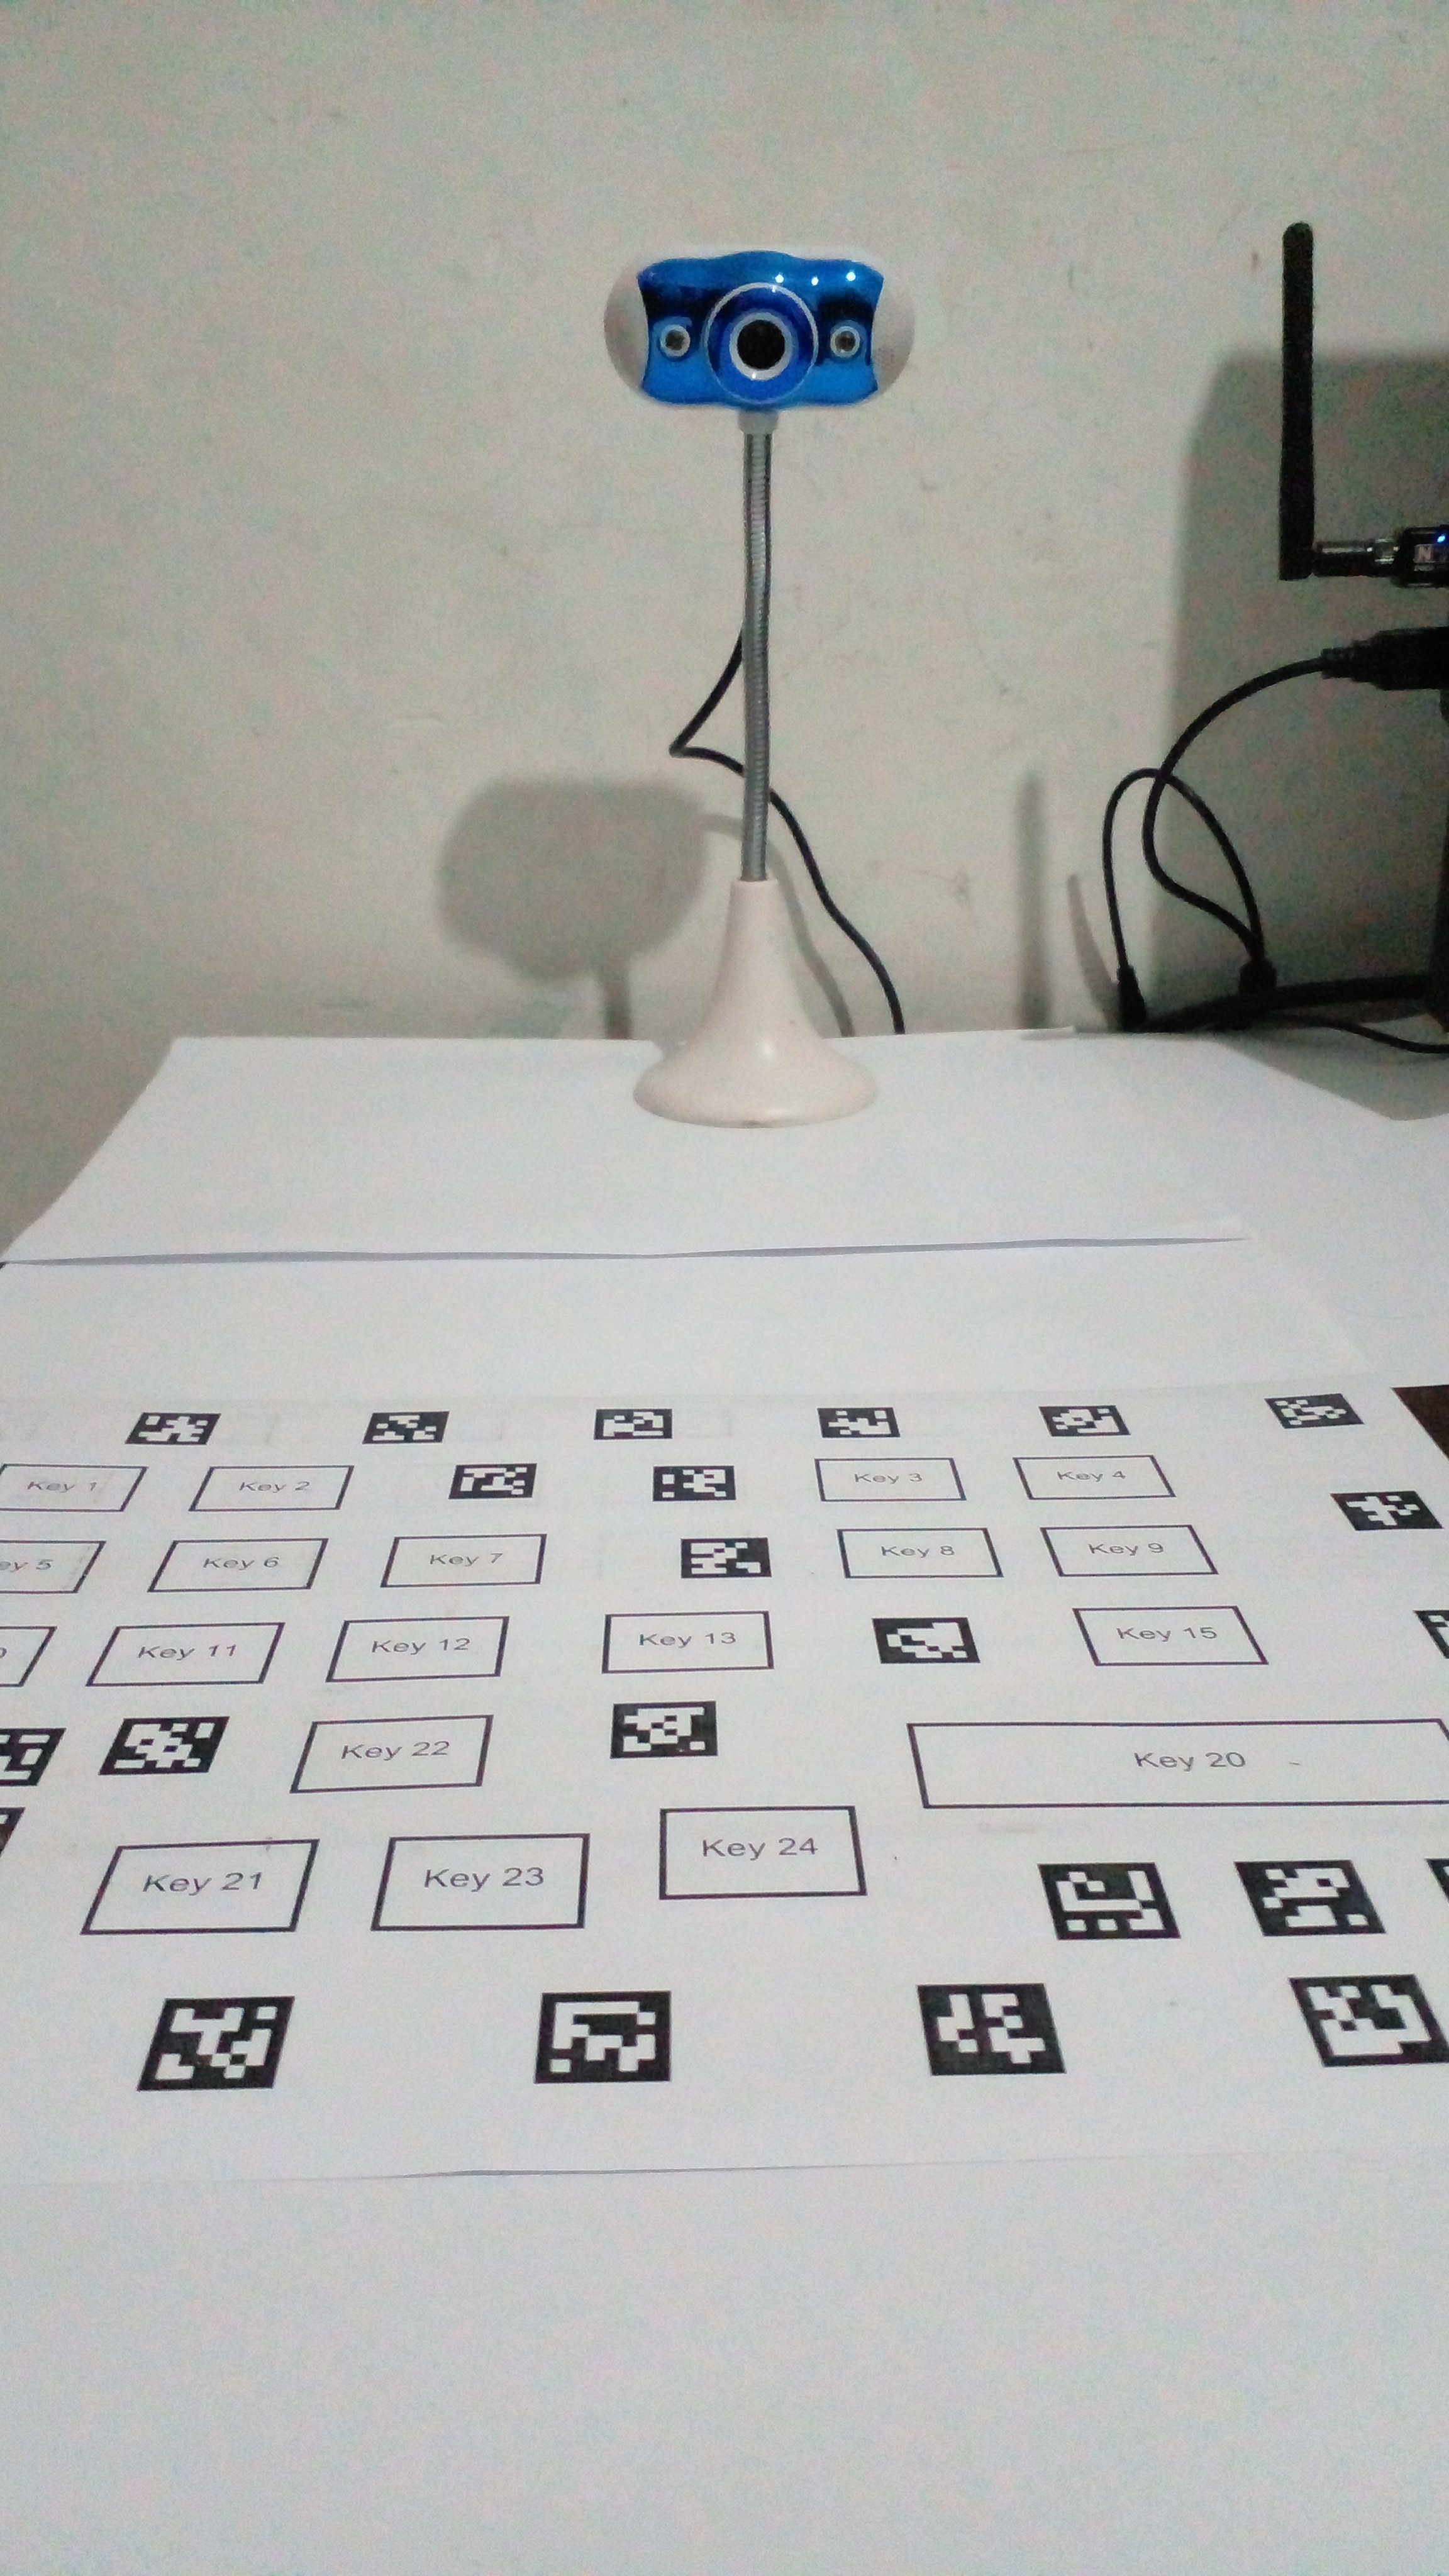
\includegraphics[width=0.72\textwidth]{figures/physical_setup_image_upright.jpg}
\caption{Physical experimental desk setup with monocular USB webcam mounted on an adjustable arm above the printed paper macro keyboard layout.}
\label{fig:appendix_physical_setup}
\end{figure}

\newpage

\section{Printable Vector Layout Artifact}
\label{sec:appendix_printable_layout}
Figure~\ref{fig:appendix_printable_pdf} shows the printable PDF layout created by Application~1 (Layout Designer). The layout is saved at 300~DPI so it prints clearly on normal A4 paper using any normal office printer. Four AprilTag markers (IDs 0, 1, 2, and 3) are placed at the corners. The middle area contains the custom macro keys with clear border lines and button names.

\begin{figure}[htbp]
\centering
\includegraphics[width=0.88\textwidth]{figures/printable_layotu_pdf_image.png}
\caption{Exported 300~DPI vector PDF layout embedded with AprilTag border fiducials ready for standard desktop paper printing.}
\label{fig:appendix_printable_pdf}
\end{figure}

\newpage
\chapter{Application 1: Paper Layout Designer Suite}
\label{ch:appendix_layout_designer}

\section{Overview of the Designer Application}
\label{sec:appendix_designer_overview}
This appendix shows screenshots of Application~1 (\texttt{virtualKeyboardSetup/}\linebreak[1]\texttt{designer/main.py}), the layout design tool built with PySide6 (developed from the initial exploratory prototype in \texttt{designer/}). Users can design custom macro keyboard layouts by dragging and dropping buttons, changing key sizes, and saving the layout as an XML coordinate file and a printable PDF document.

Figure~\ref{fig:appendix_designer_start} shows the start screen of the application. Here, users can create a new project, open a saved layout, or pick a ready-made template for shortcuts like coding or media playback.

\begin{figure}[htbp]
\centering
\includegraphics[width=0.88\textwidth]{figures/layout_designer_starting_screen.png}
\caption{Application~1 startup window for project selection and template management.}
\label{fig:appendix_designer_start}
\end{figure}

\newpage

\section{Interactive 2D Design Canvas and Property Inspector}
\label{sec:appendix_designer_canvas}
Figure~\ref{fig:appendix_designer_main} shows the main design screen. The canvas shows a standard A4 sheet in millimeters. Users can easily add, move, and resize buttons on the grid. Four AprilTags stay at the corners automatically. The side panel lets the user change key names, labels, and sizes. The software also warns the user if two keys overlap or get too close to the AprilTags.

\begin{figure}[htbp]
\centering
\includegraphics[width=0.92\textwidth]{figures/layout_designer_main_screen.png}
\caption{Application~1 interactive 2D design canvas with key layout tools, metric grid, property inspector, and AprilTag fiducial anchors.}
\label{fig:appendix_designer_main}
\end{figure}

\newpage

\section{Vector PDF Export and Print Dialog}
\label{sec:appendix_designer_export}
Figure~\ref{fig:appendix_designer_print} shows the print dialog. Users can check the preview and export the design as a high-quality 300~DPI PDF file ready to print on A4 paper.

\begin{figure}[htbp]
\centering
\includegraphics[width=0.85\textwidth]{figures/layout_designer_print_screen.png}
\caption{Application~1 export dialog for generating 300~DPI vector PDF layouts.}
\label{fig:appendix_designer_print}
\end{figure}

\newpage

\section{Designer Preferences and Snap-Grid Configuration}
\label{sec:appendix_designer_settings}
Figure~\ref{fig:appendix_designer_settings_1} and Figure~\ref{fig:appendix_designer_settings_2} show the settings windows. Users can configure paper format presets (A4 Landscape/Portrait, A3, US Letter, or custom millimeter dimensions up to $1000\text{ mm}$), border margins, grid size, snap distance, and minimum space between buttons to create clean and comfortable keypad layouts.

\begin{figure}[htbp]
\centering
\begin{subfigure}[b]{0.48\textwidth}
    \centering
    \includegraphics[width=\textwidth]{figures/layout_designer_settings_screen_1.png}
    \caption{Grid snapping and canvas preferences.}
    \label{fig:appendix_designer_settings_1}
\end{subfigure}
\hfill
\begin{subfigure}[b]{0.48\textwidth}
    \centering
    \includegraphics[width=\textwidth]{figures/layout_designer_settings_screen_2.png}
    \caption{Key dimension and margin constraints.}
    \label{fig:appendix_designer_settings_2}
\end{subfigure}
\caption{Application~1 preference settings for canvas metrics and geometric constraints.}
\label{fig:appendix_designer_settings}
\end{figure}

\newpage

\section{Exported Paper Layout XML Data Structure}
\label{sec:appendix_designer_xml}
Listing~\ref{lst:appendix_sample_xml} illustrates the structural schema of the XML layout file (\texttt{my\_paper\_keyboard.xml}) generated by Application~1 (Layout Designer) and consumed by Application~2 (Runtime Engine). The schema defines paper physical dimensions ($297 \times 210\text{ mm}$ for A4), outer margin zones, interior regions, sub-pixel four-corner metric coordinates for each printed AprilTag fiducial anchor, button bounding boxes, decoupled action mappings (\texttt{keystroke}, \texttt{shortcut}, \texttt{shell}, and \texttt{macro}), and runtime detector threshold parameters.

\begin{lstlisting}[language=XML, caption={Exported paper layout XML coordinate and action schema (\texttt{my\_paper\_keyboard.xml}).}, label={lst:appendix_sample_xml}]
<?xml version="1.0" ?>
<PaperLayout project_name="My Paper Keyboard" paper_width_mm="297.000" paper_height_mm="210.000" paper_margin_mm="10.000" marker_size_mm="15.000" marker_margin_mm="10.000" marker_spacing_mm="40.000" marker_family="DICT_APRILTAG_36h11" marker_min_gap_ratio="1.500" marker_min_gap_mm="5.000" use_custom_markers="1" show_outer_markers="1" coordinate_origin="top_left_paper_corner (x_right, y_down)" units="millimeters">
  <SystemConfig project_name="My Paper Keyboard" app_title="Virtual Keyboard Paper Layout Designer" version="1.0.0" schema_version="2.0" research_suite="Application 1 Layout Designer &amp; Application 2 Runtime Engine"/>
  <PaperMargin margin_mm="10.000" top_mm="10.000" bottom_mm="10.000" left_mm="10.000" right_mm="10.000"/>
  <MarkerRingZone outer_x_min_mm="10.000" outer_y_min_mm="10.000" outer_x_max_mm="287.000" outer_y_max_mm="200.000" inner_x_min_mm="25.000" inner_y_min_mm="25.000" inner_x_max_mm="272.000" inner_y_max_mm="185.000" marker_size_mm="15.000" marker_family="DICT_APRILTAG_36h11" marker_spacing_mm="40.000" marker_min_gap_ratio="1.500" marker_min_gap_mm="5.000"/>
  <InteriorRegion x_min_mm="30.000" y_min_mm="30.000" x_max_mm="267.000" y_max_mm="180.000" width_mm="237.000" height_mm="150.000" interior_buffer_mm="5.000"/>
  <ButtonStylingRules button_stroke_width_mm="1.000" button_corner_radius_mm="0.000" button_min_width_mm="15.000" button_min_height_mm="10.000" button_min_gap_mm="8.000" default_font_size_pt="14"/>
  <GridConfig grid_snap_enabled="1" grid_size_mm="5.000"/>
  <RuntimePipelineSpecs target_camera_fps="12" temporal_window_frames="5" temporal_window_stride="3" mediapipe_num_hands="1" mediapipe_landmarks_count="21" feature_vector_size="84" touch_model_architecture="LSTM" end_to_end_latency_ms="29.09"/>
  <Markers count="13" use_custom_markers="1">
    <Marker id="20" center_x_mm="123.500" center_y_mm="42.500" size_mm="15.000" family="DICT_APRILTAG_36h11">
      <Corners>
        <TopLeft x_mm="116.000" y_mm="35.000"/>
        <TopRight x_mm="131.000" y_mm="35.000"/>
        <BottomRight x_mm="131.000" y_mm="50.000"/>
        <BottomLeft x_mm="116.000" y_mm="50.000"/>
      </Corners>
    </Marker>
    <Marker id="21" center_x_mm="160.000" center_y_mm="45.000" size_mm="15.000" family="DICT_APRILTAG_36h11">
      <Corners>
        <TopLeft x_mm="152.500" y_mm="37.500"/>
        <TopRight x_mm="167.500" y_mm="37.500"/>
        <BottomRight x_mm="167.500" y_mm="52.500"/>
        <BottomLeft x_mm="152.500" y_mm="52.500"/>
      </Corners>
    </Marker>
    <!-- Additional AprilTag border markers 22 through 32 ... -->
  </Markers>
  <Buttons count="19">
    <Button id="btn_1" x_mm="35.000" y_mm="35.000" width_mm="25.000" height_mm="18.000" x_max_mm="60.000" y_max_mm="53.000" center_x_mm="47.500" center_y_mm="44.000">
      <Style font_size_pt="14" stroke_width_mm="1.000" corner_radius_mm="0.000"/>
      <Text>Key 1</Text>
    </Button>
    <Button id="btn_4" x_mm="220.000" y_mm="35.000" width_mm="25.000" height_mm="18.000" x_max_mm="245.000" y_max_mm="53.000" center_x_mm="232.500" center_y_mm="44.000">
      <Style font_size_pt="14" stroke_width_mm="1.000" corner_radius_mm="0.000"/>
      <Text>Key 4</Text>
    </Button>
    <Button id="btn_7" x_mm="109.000" y_mm="65.000" width_mm="25.000" height_mm="18.000" x_max_mm="134.000" y_max_mm="83.000" center_x_mm="121.500" center_y_mm="74.000">
      <Style font_size_pt="14" stroke_width_mm="1.000" corner_radius_mm="0.000"/>
      <Text>Key 7</Text>
    </Button>
    <Button id="btn_13" x_mm="146.000" y_mm="95.000" width_mm="25.000" height_mm="18.000" x_max_mm="171.000" y_max_mm="113.000" center_x_mm="158.500" center_y_mm="104.000">
      <Style font_size_pt="14" stroke_width_mm="1.000" corner_radius_mm="0.000"/>
      <Text>Key 13</Text>
    </Button>
    <!-- Additional button definitions ... -->
  </Buttons>
  <DetectorActions>
    <Actions count="19">
      <Action button_id="btn_1" label="Key 1" type="keystroke" value="r"/>
      <Action button_id="btn_4" label="Key 4" type="shortcut" value="ctrl+r"/>
      <Action button_id="btn_7" label="Key 7" type="shell" value="gnome-terminal"/>
      <Action button_id="btn_13" label="Key 13" type="macro" value="asdf"/>
      <!-- Additional action mappings ... -->
    </Actions>
  </DetectorActions>
  <DetectorSettings count="22">
    <Setting name="TARGET_FPS" value="12.0"/>
    <Setting name="TOUCH_THRESHOLD" value="0.85"/>
    <Setting name="TOUCH_ONSET_THRESHOLD" value="0.85"/>
    <Setting name="FINGERTIP_VELOCITY_THRESHOLD" value="0.2000"/>
    <Setting name="MIN_KINETIC_SPEED_THRESHOLD" value="0.2000"/>
    <Setting name="HAND_MOVEMENT_THRESHOLD" value="0.2000"/>
    <Setting name="MEDIAPIPE_MIN_DETECTION_CONFIDENCE" value="0.60"/>
    <Setting name="MEDIAPIPE_MIN_PRESENCE_CONFIDENCE" value="0.60"/>
    <Setting name="MEDIAPIPE_MIN_TRACKING_CONFIDENCE" value="0.50"/>
    <Setting name="QUALITY_MIN_AVG_SCORE" value="0.60"/>
    <Setting name="QUALITY_MIN_FRAME_SCORE" value="0.60"/>
    <Setting name="QUALITY_MAX_SCORE_DROP" value="0.35"/>
    <Setting name="FINGERTIP_OFFSET_ENABLED" value="true"/>
    <Setting name="FINGERTIP_FORWARD_OFFSET_MM" value="5.00"/>
    <Setting name="TOUCH_RELEASE_WINDOWS" value="2"/>
    <Setting name="TOUCH_MAX_STATIONARY_DISTANCE_MM" value="4.0"/>
    <Setting name="PRINTED_MARKER_SIDE_WIDTH_MM" value="15.00"/>
  </DetectorSettings>
</PaperLayout>
\end{lstlisting}

\newpage
\chapter{Application 2: Runtime Virtual Keyboard Engine and Live Tracking}
\label{ch:appendix_detector_runtime}

\section{Overview of the Runtime Engine}
\label{sec:appendix_detector_overview}
This appendix shows screenshots of Application~2, which is the runtime virtual keyboard program. This application tracks the AprilTag markers, tracks hand joints using MediaPipe, detects finger touches using our PyTorch LSTM model, and runs the assigned keyboard shortcuts.

Figure~\ref{fig:appendix_detector_home} shows the start screen where the user selects the webcam, loads the layout XML file, and chooses an action profile.

\begin{figure}[htbp]
\centering
\includegraphics[width=0.88\textwidth]{figures/detector_home_screen.png}
\caption{Application~2 home screen for camera device selection and layout loading.}
\label{fig:appendix_detector_home}
\end{figure}

\newpage

\section{Action Rebinding and Profile Management}
\label{sec:appendix_detector_rebinding}
Figure~\ref{fig:appendix_detector_edit} shows the action rebinding window. Users can change the action of any key to standard keyboard shortcuts (like Ctrl+C or Alt+Tab) or terminal scripts. Both applications use the exact same XML file, saving key actions and detector settings directly into the \texttt{<DetectorActions>} and \texttt{<DetectorSettings>} sections of the layout XML. This removes the need for separate files, allowing users to switch between different XML action profiles on the same printed paper sheet without printing again.

\begin{figure}[htbp]
\centering
\includegraphics[width=0.92\textwidth]{figures/detector_layout_edit_mode.png}
\caption{Application~2 action rebinding interface for assigning keystrokes and shell commands to macro keys.}
\label{fig:appendix_detector_edit}
\end{figure}

\newpage

\section{Live Camera Tracking in Idle and Contact States}
\label{sec:appendix_detector_live_states}
Figure~\ref{fig:appendix_detector_idle} shows the live camera view when no hand is present. The software finds the four AprilTags at the corners, calculates the homography matrix $H$, and draws the key boxes onto the camera video.

\begin{figure}[htbp]
\centering
\includegraphics[width=0.88\textwidth]{figures/detector_playmode_without_hand_just_idle.png}
\caption{Application~2 idle monitoring state showing detected AprilTags, homography alignment, and key bounding boxes.}
\label{fig:appendix_detector_idle}
\end{figure}

Figure~\ref{fig:appendix_detector_touch} shows what happens when a finger touches a key. MediaPipe tracks the 21 hand joints in real time. When the index finger hits the paper, our PyTorch LSTM model predicts a 96\% touch probability for the index finger. The program calculates which key was touched, highlights the key in green on the screen, and sends the keystroke to the computer.

\begin{figure}[htbp]
\centering
\includegraphics[width=0.88\textwidth]{figures/detector_playmode_exacty_index_finger_touch_happening_on_a_key.png}
\caption{Application~2 live contact detection showing MediaPipe skeleton, 96\% index touch probability, and highlighted key impact.}
\label{fig:appendix_detector_touch}
\end{figure}

\newpage

\section{Production Run Mode and Action Event Log}
\label{sec:appendix_detector_run_mode}
Figure~\ref{fig:appendix_detector_run} shows the live run mode. A line graph shows the touch probabilities for each finger over time. The screen shows that the program runs smoothly at 11.9~FPS with an inference time of only 2.3~ms on the CPU. The list on the right shows recent key presses.

\begin{figure}[htbp]
\centering
\includegraphics[width=0.92\textwidth]{figures/detector_run_mode_multipl_touches_happend.png}
\caption{Application~2 production run mode showing real-time multi-finger probability history, pipeline FPS, and action event log.}
\label{fig:appendix_detector_run}
\end{figure}

\newpage

\section{Runtime Engine Preferences and Detection Parameters}
\label{sec:appendix_detector_settings}
Figure~\ref{fig:appendix_detector_settings_1} and Figure~\ref{fig:appendix_detector_settings_2} show the settings screens. Users can change the touch threshold ($\tau_{\text{touch}}$), delay times between presses, and camera update rates.

\begin{figure}[htbp]
\centering
\begin{subfigure}[b]{0.48\textwidth}
    \centering
    \includegraphics[width=\textwidth]{figures/detector_settings_page_1.png}
    \caption{Touch sensitivity and classification thresholds.}
    \label{fig:appendix_detector_settings_1}
\end{subfigure}
\hfill
\begin{subfigure}[b]{0.48\textwidth}
    \centering
    \includegraphics[width=\textwidth]{figures/detector_settings_page_2.png}
    \caption{Homography smoothing and dispatch settings.}
    \label{fig:appendix_detector_settings_2}
\end{subfigure}
\caption{Application~2 configuration settings for vision tracking and touch triggering.}
\label{fig:appendix_detector_settings}
\end{figure}

\newpage
\chapter{Ground-Truth Dataset Annotation Platform}
\label{ch:appendix_data_annotator}

\section{Overview of the Annotation Suite}
\label{sec:appendix_annotator_overview}
This appendix shows screenshots of the dataset annotation program we built to label touch events in recorded videos. Getting correct touch labels frame by frame was important to train and test our PyTorch neural network model.

Figure~\ref{fig:appendix_annotator_home} shows the start screen of the tool, where we select video files and keyboard layout settings to begin labeling.

\begin{figure}[htbp]
\centering
\includegraphics[width=0.88\textwidth]{figures/data_annotator_home_page.png}
\caption{Dataset annotation tool home screen for video session management.}
\label{fig:appendix_annotator_home}
\end{figure}

\newpage

\section{Frame-by-Frame Skeletal Annotation Interface}
\label{sec:appendix_annotator_workspace}
Figure~\ref{fig:appendix_annotator_main} shows the main labeling screen. Recorded videos are played frame by frame at 12~FPS. MediaPipe 21 hand joints are drawn directly over the hand. The buttons on the right let us mark whether each finger (Thumb, Index, Middle, Ring, Pinky) is touching the paper or not in each frame.

\begin{figure}[htbp]
\centering
\includegraphics[width=0.92\textwidth]{figures/data_annotator_main_screen_live_annotation.png}
\caption{Dataset annotator main interface showing 12~FPS frame navigation, MediaPipe skeleton overlay, and per-digit contact labeling.}
\label{fig:appendix_annotator_main}
\end{figure}

\newpage

\section{Rapid Keyboard Shortcuts for Annotation Efficiency}
\label{sec:appendix_annotator_shortcuts}
Figure~\ref{fig:appendix_annotator_shortcuts} shows the keyboard shortcuts dialog in the annotator. Since we had to label thousands of frames, we added quick keyboard shortcuts (like keys 1 to 5 to toggle fingers, and spacebar to move to the next frame). This made labeling much faster and easier.

\begin{figure}[htbp]
\centering
\includegraphics[width=0.85\textwidth]{figures/data_annotator_shorcut_window.png}
\caption{Keyboard shortcut dialog enabling rapid multi-finger ground truth tagging during video annotation.}
\label{fig:appendix_annotator_shortcuts}
\end{figure}

\newpage
\chapter{Empirical Model Benchmarking and Latency Profiling}
\label{ch:appendix_evaluation_benchmarks}

\section{Overview of Empirical Benchmark Charts}
\label{sec:appendix_benchmarks_overview}
The following figures in this appendix are the graph and chart representations of the experimental results analysis covered in Chapter~\ref{ch:results}. They include comparisons among deep learning methods, confusion matrices for each finger, accuracy of AprilTag homography tracking in terms of tilt angles, and runtime CPU latency.

\section{Model Architecture Accuracy versus CPU Latency}
\label{sec:appendix_model_benchmark_chart}
The Macro F1-score and CPU inference time of various deep learning architectures have been compared in Figure~\ref{fig:appendix_benchmark_acc} of the current benchmark test. The uni-directional LSTM with scale-normalized position and velocity scores best among all architectures with an F1-score of 0.963 and CPU inference time of $2.08\text{ ms}$ on the CPU.

\begin{figure}[htbp]
\centering
\includegraphics[width=0.88\textwidth]{figures/fig_model_benchmark_acc.png}
\caption{Comparison of Macro F1-score and CPU inference latency across evaluated deep learning model architecture families.}
\label{fig:appendix_benchmark_acc}
\end{figure}

\newpage

\section{Per-Digit Touch Confusion Matrix}
\label{sec:appendix_confusion_matrix_chart}
As shown in Figure~\ref{fig:appendix_confusion_matrix}, the normalized confusion matrix for our chosen PyTorch LSTM model was generated using 5,000 test windows. All five fingers have touch detection accuracies greater than 93\%. The highest accuracy belongs to the index finger (99.0\% recall), while the pinky finger is slightly lower due to its smaller movement.

\begin{figure}[htbp]
\centering
\includegraphics[width=0.82\textwidth]{figures/fig_confusion_matrix.png}
\caption{Normalized confusion matrix of the PyTorch LSTM touch classifier across all five individual finger digits.}
\label{fig:appendix_confusion_matrix}
\end{figure}

\newpage

\section{AprilTag Homography Tracking Under Perspective Tilt}
\label{sec:appendix_homography_tilt_chart}
The influence of camera tilt angles (ranging from $0^\circ$ to $75^\circ$) on AprilTag tracking is presented in Figure~\ref{fig:appendix_homography_tilt}. The corner detection percentage remains close to 100\%, while the average tracking error remains at less than $0.42\text{ mm}$ for angles ranging from $0^\circ$ to $60^\circ$ of the desk. Beyond $65^\circ$, there is an increase in error due to perspective tilt, showing that $0^\circ$ to $60^\circ$ is the best angle range.

\begin{figure}[htbp]
\centering
\includegraphics[width=0.88\textwidth]{figures/fig_homography_tilt_error.png}
\caption{AprilTag corner detection rate and RMS planar reprojection error across camera perspective tilt angles.}
\label{fig:appendix_homography_tilt}
\end{figure}

\newpage

\section{Multi-Threaded Real-Time Pipeline Latency Breakdown}
\label{sec:appendix_latency_breakdown_chart}
As can be seen in Figure~\ref{fig:appendix_latency_breakdown}, this represents the time required for each pipeline stage to execute itself on an Intel Core i7 processor. Total time required for processing is $29.09\text{ ms}$ (approximately $34.4\text{ FPS}$). It utilizes only about 35\% of the total possible $83.33\text{ ms}$ budget at 12~FPS, which means the program runs smoothly in real time without needing a GPU.

\begin{figure}[htbp]
\centering
\includegraphics[width=0.88\textwidth]{figures/fig_latency_breakdown.png}
\caption{End-to-end CPU execution latency breakdown per frame across the multi-threaded virtual keyboard pipeline.}
\label{fig:appendix_latency_breakdown}
\end{figure}


\end{document}
